% Two sided means the left and right margins are different sizes and they alternate every page.
% If your document is printed to be book or spiral bound this allows for a thick spine to not
% eat into the space for your page content.
\documentclass[11pt, a4paper, oneside]{custard}

\usepackage{geometry}
\usepackage[utf8]{inputenc}
\usepackage[T1]{fontenc}
\usepackage{pdflscape}
\usepackage{afterpage}
\usepackage{enumitem}
\usepackage{wrapfig}
% \usepackage{hyperref}
\geometry{
	a4paper,
	left   = 30mm,
	right  = 30mm,
	top    = 30mm,
	bottom = 30mm
}
\usepackage{todonotes}

% All imports, packages, and configuration in here.
% Your document should be about content so we abstract away the styling rules and tools we are using.
%% Here you can specify new commands and environments that you intend
%% to use. Using commands can make your document easier to write, read
%% and be more consistent.

\usepackage[linesnumbered,ruled]{algorithm2e}
\DeclareMathOperator*{\argmin}{arg\,min}

\usepackage{diagbox}
\usepackage{appendix}
\usepackage{textcomp}
\usepackage{setspace}
%\usepackage[document]{ragged2e}
\usepackage{verbatim}
\usepackage{multirow}
\usepackage{multicol}
\usepackage{booktabs}
\usepackage{enumitem}
\sloppy
\usepackage{graphicx}
\usepackage{threeparttable}
\usepackage{epsfig}
\usepackage{epstopdf}
\usepackage{float}
\usepackage{enumitem}
\usepackage{cite}
\usepackage[export]{adjustbox}
\usepackage{algorithmic}
\usepackage[nohyperlinks,printonlyused]{acronym}
\usepackage{amsmath}
\usepackage{amsfonts}
\usepackage{array}
\usepackage{tabularx}
\usepackage{xltabular}
\usepackage{longtable}
\usepackage{times}
\usepackage{amssymb}
\usepackage{hhline}
\usepackage{color}
\usepackage{soul}
\usepackage{colortbl}
\definecolor{Gray}{gray}{0.85}
\usepackage{rotating}
\usepackage{fix2col}
\usepackage{pdflscape}
\usepackage{pdfpages}
\usepackage{stmaryrd}
\usepackage[export]{adjustbox}
\usepackage{bbm}
\usepackage{relsize}
\usepackage{xfrac}
\usepackage{bibentry}

%\usepackage{refcheck}

%watermarking
\usepackage[english]{babel}
\usepackage{tikz}

%% Uncomment the following line for hyper links - not recommended for printing
\usepackage[colorlinks, linkcolor=, anchorcolor=, citecolor=, filecolor=, menucolor=, runcolor=, urlcolor=]{hyperref}

\setcounter{tocdepth}{1}
%\setcounter{minitocdepth}{3}
\linespread{1.31}

\newcommand\litem[1]{\item{\bfseries #1:\enspace}}

\interdisplaylinepenalty=2500

\newcolumntype{L}[1]{>{\raggedright\let\newline\\\arraybackslash\hspace{0pt}}m{#1}}
\newcolumntype{C}[1]{>{\centering\let\newline\\\arraybackslash\hspace{0pt}}m{#1}}
\newcolumntype{R}[1]{>{\raggedleft\let\newline\\\arraybackslash\hspace{0pt}}m{#1}}

\renewcommand{\thefootnote}{\fnsymbol{footnote}}
\setlength{\LTpre}{-10pt}\setlength{\LTpost}{-30pt}%
\newcommand{\oiint}{\begin{picture}(0,0)(-10,-2)\put(0,0){\oval(12,8)}\end{picture}\iint}
\renewcommand{\mathbf }{\boldsymbol}

\def \eg{e.g.\ } % Allows you to write \eg in LaTeX instead of typing e.g. so that every single one will be formatted the same.
\def \Eg{E.g.\ } % Define some other common variants. If you later want to change one of these definitions,
\def \ie{i.e.\ } % it will update all the usages throughout the document.
\def \Dr{Dr.\ }
\def \vs{vs. }
\def \etal{\emph{et al.\ }}
\def \sota{state-of-the-art }
\def \handcrafted{hand-crafted }

\usepackage{listings,lstautogobble}
\usepackage{sourcecodepro}
\pdfmapfile{=SourceCodePro.map}
\lstset{
	xleftmargin=0.5cm,frame=tlbr,framesep=4pt,framerule=0.5pt,
	language=,
	upquote=true,
	columns=fixed,
	tabsize=2,
	extendedchars=true,
	breaklines=true,
	numbers=left,
	numbersep=10pt,
	basicstyle=\ttfamily\scriptsize,
	numberstyle=\tiny,
	stringstyle=\ttfamily,
	captionpos=b,
	showstringspaces=false,
	autogobble=true
}

\usepackage[font=small,skip=10pt]{caption} %,format=hang
%\usepackage[labelformat=simple]{subcaption}
\usepackage[labelformat=simple]{subfig}
%\captionsetup[figure]{format=hang}
%\captionsetup[lstlisting]{format=hang}
\renewcommand{\thesubfigure}{\Alph{subfigure}.}

\renewcommand{\thefootnote}{\arabic{footnote}}

% Use IEEEtran citation style.
\bibliographystyle{IEEEtran}

\def\samplefont#1{%
    % set font style and save name
    #1\edef\savedname{\fontname\font}%
    % print small sample
    {\leavevmode\tt\hbox to 1in{\savedname:\hss}}%
    abcxyz ABCXYZ 123\par
}


\begin{document}

% The custom data for Swansea University and your degree name.
% The \protect\\ command forces a new line in the title which might be otherwise overriden by the template
	\title{Walking Aid Usage Prompt System}
	\author{Pedro Caetano, Matthew Culley, Sean Coaker, Panayiotis Melios}
	\awardinginst{Swansea University}
	% Comment / uncomment your degree type as needed.
	\degree{Masters of Science/Engineering}

% Institution details and logo
	\department{Faculty of Science and Engineering}
	\university{Swansea University}
	\unilogo{graphics/swansea.png}

% Hard code the date or allow the LaTeX compiler to fill it in whenever you recompile the document.
	\date{\today}

% Build the title and declaration pages, and pad the document so the text starts on a right hand book page.
% Page numbering is in roman numerals until the first page of an actual chapter which resets numbers
% starting from 1 at that point.
	\frontmatter%
	\maketitle
	%generate list of todos
	%\setcounter{secnumdepth}{2}
	%\setcounter{tocdepth}{2}
	\listoftodos
	\tableofcontents

% Optionally you can make a bank of known acronyms in acronyms.tex that you can call on throughout your document.
	%\input{acronyms}

% Reset numeric page numbering from page 1
	\mainmatter%

% Insert the code for each of your chapters
	\chapter{Design}
\label{ch:design}

    This chapter will detail the design decisions made for the project's hardware and software systems, that ultimately led to us being able to successfully implement our systems and meet the original requirements set out by our clients. The following sections will break down our final product into two systems, the walking aid device and the wearable device, detailing the design decisions made for each system, including which technologies were used and UML diagrams of the systems. We will begin by detailing the design choices we made that impact both systems before breaking down our design decisions that individually impact the walking aid and wearable devices.

    \section{Walking Aid Device}
    \label{sec:walking_aid}

        The walking aid device is a device that can be used to detect movement of the walking aid. When the wearable device detects that the patient is walking, a message is sent to the walking aid device. Should the walking aid device detect that it is not moving when the patient is walking, it will play an audio reminder to the patient to take their walking aid with them. The following sections will detail the design choices we made for this system, where we will compare technologies that would have been suited to the system and which we chose to implement, as well as a UML design section which will include a class diagram of the developed software system and an activity diagram that demonstrates the workflow of the software that allows the device to meet our desired specification.

        \subsection{I2S Audio Shield}
        \label{subsec:i2s_audio_shield}

            For the purposes of handling the amplification of reminder audio files and transferring the analogue data of the reminder audio to an external speaker, we needed to select an audio shield. In this instance we selected the I2S Audio Shield \cite{unexpected_maker} on offer from Unexpected Maker, the creator of the TinyPICO development board that has been previously mentioned in section \ref{subsec:development_board}. What attracted the team to using this particular audio shield was the fact that it already included the necessary hardware for handling the audio reminder system. That is that it contains a micro-SD card slot for the reading of the user's reminder audio file, external speaker output pins, and an amplifier to increase the volume of the audio in readiness to be transferred to the external speaker. With all these hardware devices housed on one audio shield, it made the design of the walking aid device casing more simple than an alternative that may have needed separate modules for the amplification of audio and the reading of a microSD card. In addition to this, our assumption was that acquiring separate hardware items from the same manufacturer would lead to a greater chance of our hardware devices communicating flawlessly with each other. To this end, we have not experienced any issues with the communication between the walking aid's TinyPICO and its audio shield. Therefore, we would say that in this instance, our assumption was correct.
            
            Alternative solutions could have taken the form of utilising the same ``MAX98357 I2S Decoder and Amp'' \cite{unexpected_maker} as the one used by the I2S Audio Shield we selected, but instead combining it with a separate dedicated micro-SD card reader, such as this offering \cite{ada_2022} from the well known embedded hardware manufacturer, Adafruit. The wiring and code development in this instance would have been identical, but we appreciated the fact that the Unexpected Maker solution houses the I2S decoder and amplifier on the same board as the microSD card reader. Along with this, the I2S audio shield is of a similar form factor to the TinyPICO development board and made the 3D modelling and printing process a simpler process.

        \subsection{SD Card Reading Library - SdFat}
        \label{subsec:sdfat}

            The decision to use the SdFat library by Bill Greiman \cite{greiman} was an unexpected one as Arduino provide their own solution of SD card reading library \cite{arduino} which acts as a wrapper to the SdFat library for easier understanding and further abstraction of the underlying code. However, when testing the transfer of an 150 KB mp3 file to the SPIFFS storage location of the TinyPICO, we began to notice that the library was taking an abnormally long time to complete the process, especially with a file this small. Upon completing research on the transfer speeds of the Arduino SD library, it was clear to see that the library had not been tested or optimised adequately enough to be used for the fast transferring of audio files from the microSD card to SPIFFS within our walking aid device. Discussion of these issues are widespread \cite{fat16lib_2011,drdooom_2019} with one GitHub user claiming that the SdFat library is ``85 times faster'' \cite{kas2_2018} than the Arduino SD library. Our own testing demonstrated transfer times of the 150 KB mp3 file from the microSD card to SPIFFS at around 150 seconds for the Arduino SD library, and around 12 seconds for the SdFat library. More information on this is viewable within the testing section of this document. But with such a stark difference in transfer rates, and with fast transfer rates being crucial for the prompt initialisation of our systems, we felt that the SdFat library was the most appropriate solution for our purposes.

        \subsection{Physical Design}
        \label{subsec:Design_Decisions_walking_aid}

            \todo{Check for self-plagiarism}
            Upon clarifying the physical needs and requirements of the device, it was decided that the walking aid device had to be adaptable between different walking aids, such as a walking sticker or Zimmer frame. Form factor was a specially important priority, as a small/minimal footprint would minimise any potential problems or complications with the users. With this in mind, and with components at hand, the design was made with minimal overhead over the physical size of the items we had at hand. 

            \begin{figure}[H]
\centering
\begin{minipage}{.5\textwidth}
  \centering
  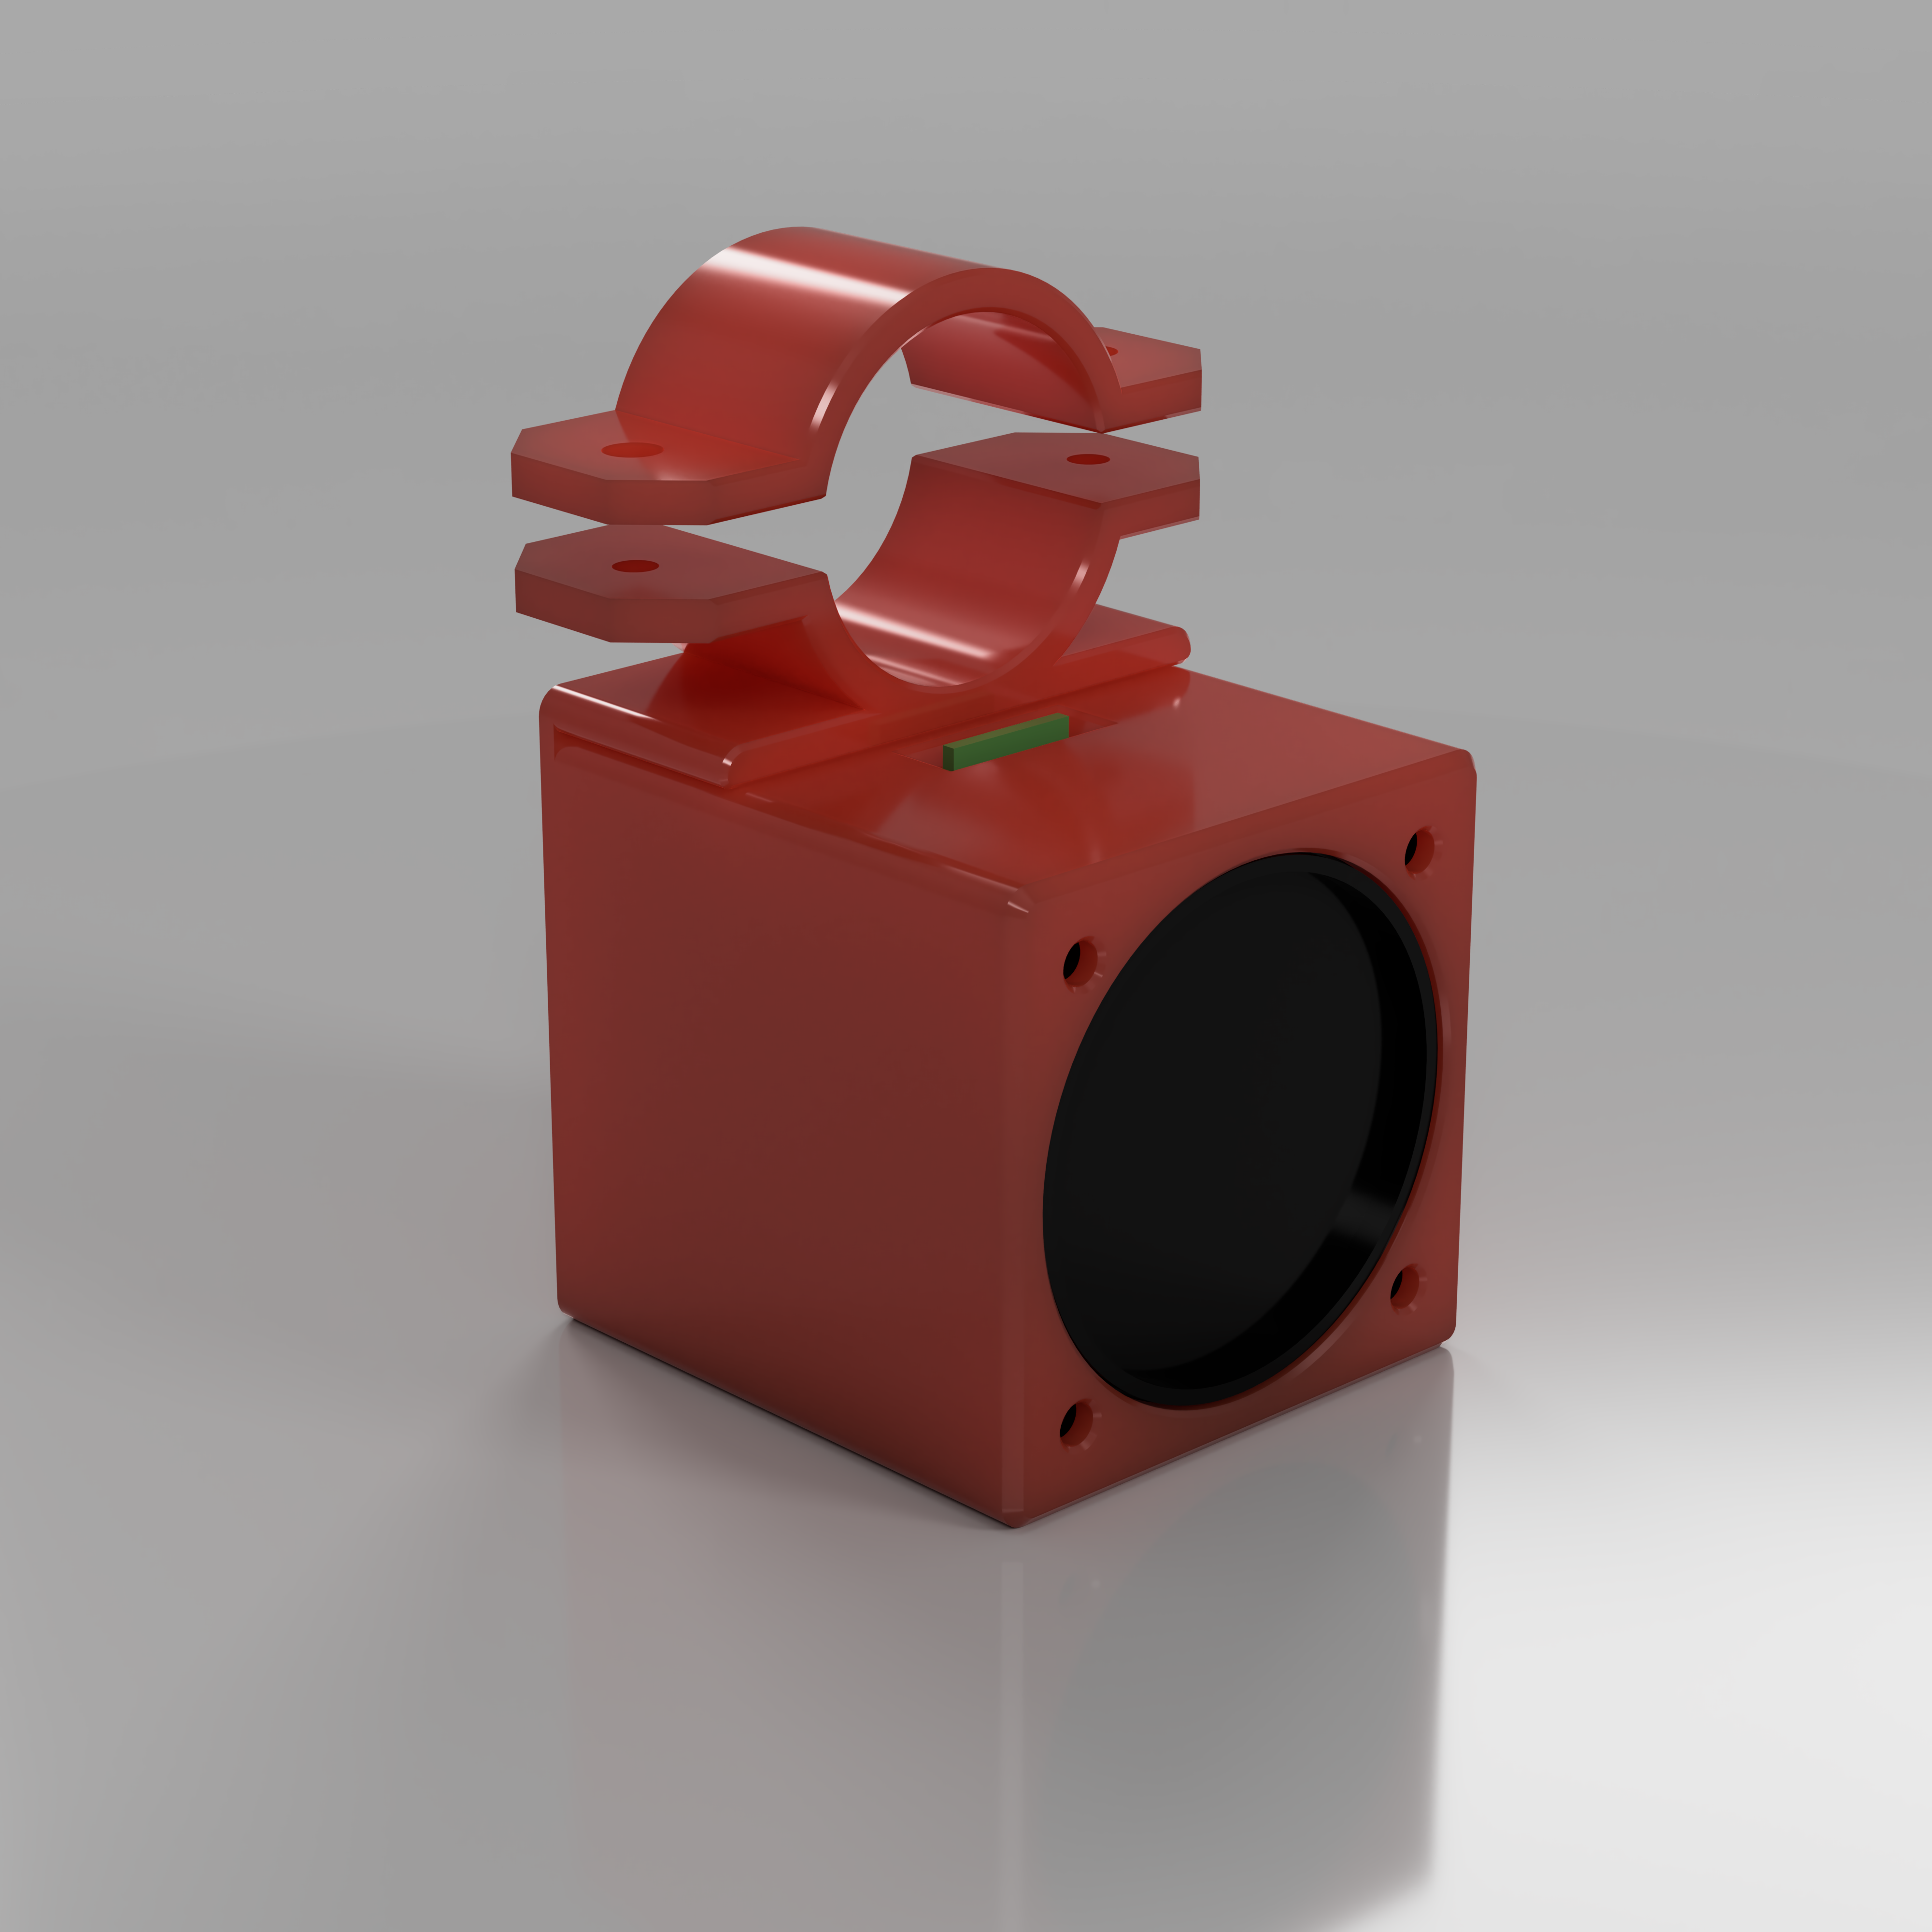
\includegraphics[width=.8\linewidth]{graphics/cad/walkingaid_1.png}
  \captionsetup{width=0.8\linewidth, justification=centering}
  \centering
  \captionof{figure}{Assembled walking aid device}
  \label{fig:walkingaid_1}
\end{minipage}%
\begin{minipage}{.5\textwidth}
  \centering
  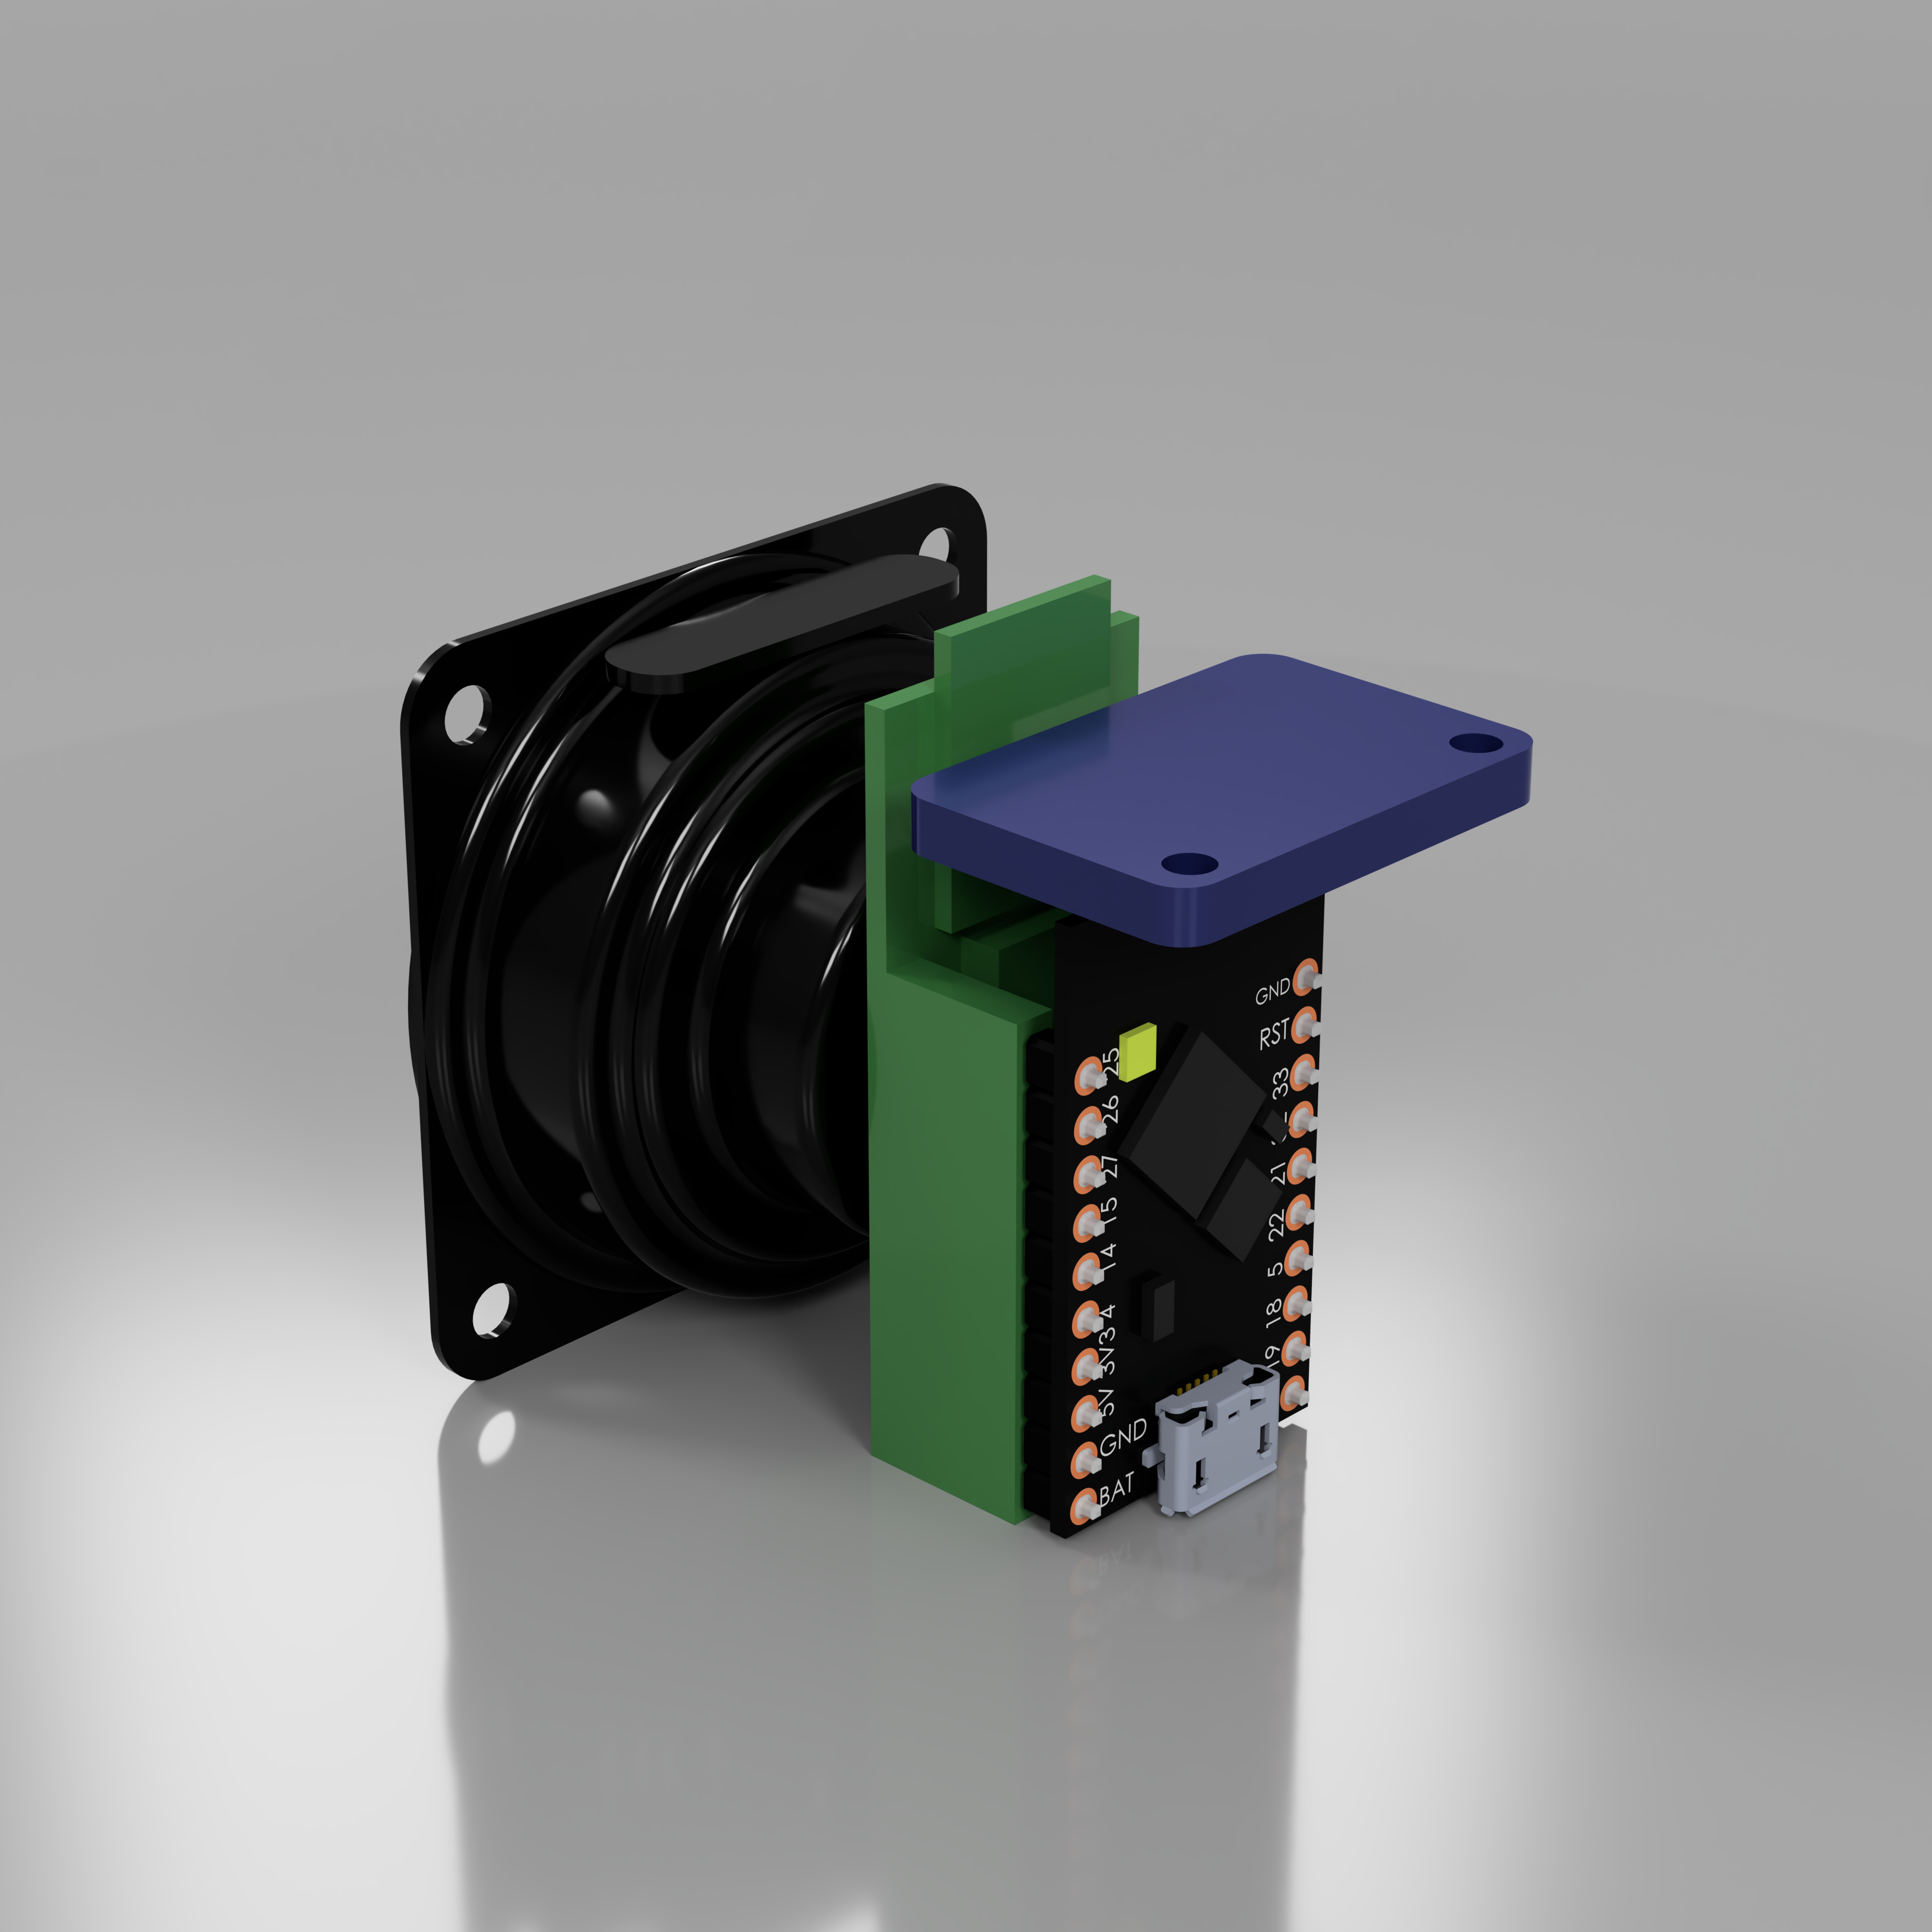
\includegraphics[width=.8\linewidth]{graphics/cad/walkingaid_components_1.png}
  \captionsetup{width=0.8\linewidth, justification=centering}
  \centering
  \captionof{figure}{Walking aid device component layout}
  \label{fig:walkingaid_components_1}
\end{minipage}
\end{figure}

            The design was made as modular as possible, to allow for changeable parts, to make it inter-operable different walking aids and mounting/battery options. The mounting options were inspired from the GoPro style of handlebar mount, this was chosen due to its simplicity, and the sturdiness of attachment which will help with the reading from our accelerometers. The mount was scaled down to more appropriately attach to a walking stick or Zimmer frame, but as mentioned can be easily swapped and modified to work with bigger or smaller tubes/frames.

            In order to fulfil the specification, and allow for familiar voices to remind the users, a MicroSD card was chosen as described above. This required easy access to the card slot, which had to be intuitive and accessible without disassembly of the device.

            Further considerations include easy access to the microUSB port. This port is required for programming/updating the device, as well as be an option for powering the device if no battery is wanted/needed, or a 5v source is available (such as a large, portable powerbank).

            As noted, the current prototype has no battery support, but the design decision for this walking aid device is to offer swappable endcases, this helps with modularity to allow for different mounts and attachments, but with a through hole for wiring, als allows for future implementations of battery based sources, such as replaceable batteries or rechargeable internal cells.

        \subsection{UML}
        \label{sec:uml_walk_aid}
        
            This section will break down the software systems utilised in the walking aid device into formal language representations. These will take the form of a class diagram, which will illustrate the relationships between each of classes developed for the system, and an activity diagram which will demonstrate the sequence of events that will take place in the system and how they are handled. We hope that this section will help the reader to understand the software system in a broken down, step-by-step manner and to gain an understanding of our rationale towards programming choices that helped us to fulfil the user requirements. The class diagrams will be followed by an explanation of the role of each class and its functions, with the activity diagram also being accompanied by a body of text that establishes in natural language the sequence of events that will take place in the software system and how they are processed.

            \subsubsection{Class Diagram}
            \label{subsubsec:class_diagram_walking_aid}

                To demonstrate how the classes within the software are laid out and how they communicate with one another to make up the whole system, we include here a class diagram. Following the class diagram, we will include documentation on each class and their functions towards benefitting the functionality of the system. 

                \clearpage
                \thispagestyle{empty}
                \begin{landscape}
                    % [H] means put the figure HERE, directly when you input this code.
\begin{figure}[ht!]
	\centering
	\captionsetup{width=1.0\linewidth}

% We set the width of the figure based on the width of one line of text on the page.
% The value can be tuned to any value in [0.0, 1.0] to scale the image while maintaining its aspect ratio.

	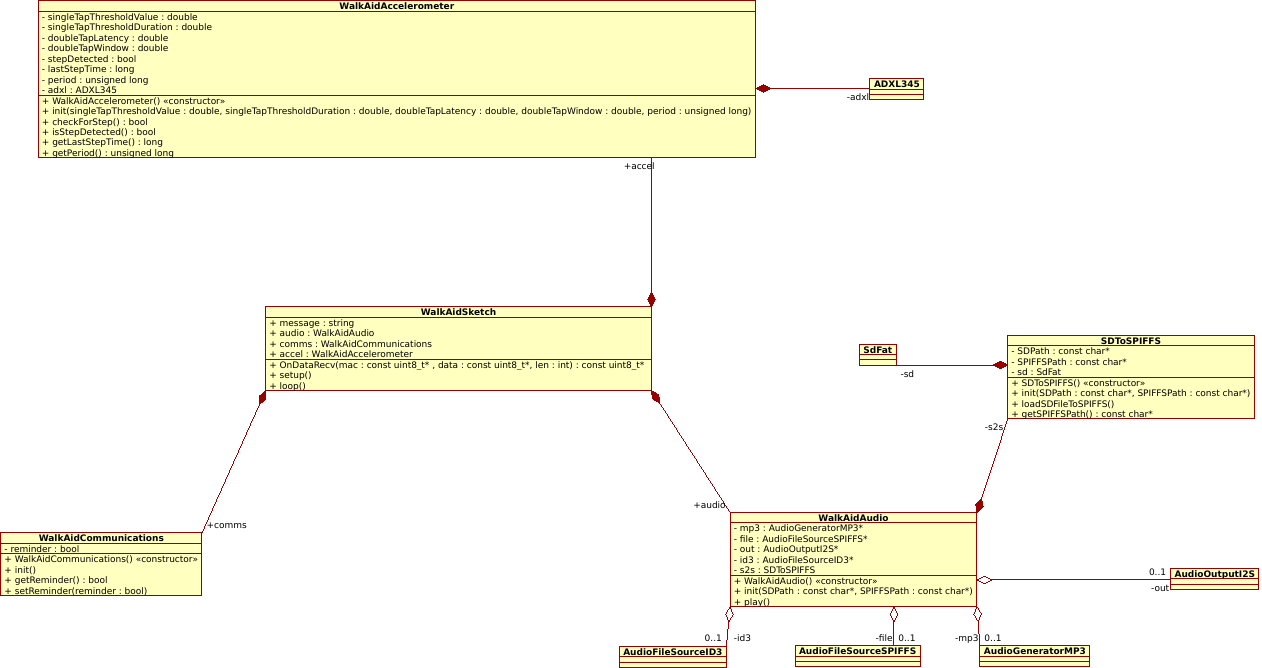
\includegraphics[width=1.0\linewidth]{./UML/WalkingAidDevice/class diagram.png}

% Caption is defined with a short and long version. The short version is shown in the
% List of Figures section, and the long version is used directly with the figure.
	\caption[Walking Aid Device Class Diagram]{A class diagram for the walking aid device software system illustrating how the classes interact with each other.}

% For figures label should be defined after the caption to ensure proper figure numbering.
	\label{fig:class_diagram_walking_aid}

\end{figure}
                \end{landscape}

                \paragraph{WalkAidSketch}\mbox{}

                    This is the main controller of the whole walking aid system and provides the functionality of the setup and loop functions that are required by Arduino systems. It has a composition relationship with the WalkAidAccelerometer, WalkAidCommunications, and the WalkAidAudio classes. Thus, the WalkAidSketch class cannot function without the existence of those classes, and those classes cannot function without the existence of the WalkAidSketch class. The WalkAidSketch class handles the initialisation of the other classes within the setup function, before ensuring that each time the loop function is called, checks are made to see if reminder messages have been received and if so, are responded to accordingly.

                \paragraph{WalkAidAccelerometer}\mbox{}

                    The WalkAidAccelerometer class is responsible for the initialisation of the accelerometer, and the reading of the accelerometer data. The class keeps track of when a step was last taken to avoid the audio reminder being played if the walking aid is moving. It has a composition relationship with the ADXL345 class meaning that neither class could function properly without the existence of each other. This class also relies on the existence of the WalkAidSketch to exist itself.

                \paragraph{WalkAidCommunications}\mbox{}

                    The WalkAidCommunications class is responsible for the initialisation of the ESP-Now communication protocol to establish a connection to the wearable device. When a reminder message is received, the reminder variable is set to true to allow the WalkAidSketch to check for a step in the previous period of time or in the future period of time. Should a reminder need to be played but the user is deaf, this class will send a message back to the wearable device prompting it to vibrate. This class is initialised in the WalkAidSketch class and does not exist unless that class exists. Therefore, it is part of a composition relationship with the WalkAidSketch.

                    The WalkAidCommunications class also makes use of the DebugLED class to ensure that the user is notified of any issues in initialising the communications protocol on boot. It has a composition relationship with the DebugLED class to allow for the LED to be configured should an error occur with the initiation of the communication protocol.

                \paragraph{DebugLED}\mbox{}

                    The DebugLED class exists to handle the configuration of the TinyPICO's onboard LED to indicate whether the communication protocol is working or not. It is initialised in the WearableDeviceSketch class and is therefore part of a composition relationship with the WearableCommunications class. More specifically, an instance of the DebugLED class cannot exist without an instance of the WearableCommunications class.

                    The DebugLED class also holds a composition relationship with the TinyPICO helper library to allow for the configuration of the LED.

                \paragraph{WalkAidAudio}\mbox{}

                    This class handles the initialisation of the SDToSPIFFS class to allow for the transferring of an audio SD file to the SPIFFS memory. Afterwards, it initialises all the necessary classes to interpret the mp3 audio file and play it. This class creates pointers to the AudioFileSourceID3, AudioFileSourceSPIFFS, AudioGeneratorMP3, and AudioOutputI2S classes. It has an aggregation relationship with these classes as it is responsible for their deletion due to them being pointer variables. It also holds a composition relationship with the SDToSPIFFS class, which is utilised for the transferring of the audio file from the SD card to the SPIFFS storage. 

                \paragraph{SDToSPIFFS}\mbox{}

                    This class is responsible only for the transferring of the SD card audio file to the SPIFFS storage. It is part of a composition relationship with the WalkAidAudio class, due to it relying on being initialised in that class to exist. It also holds a composition relationship with the SdFat class, which we discussed in section \ref{subsec:sdfat}, to handle the more intricate SD card functions. 
                
                \newpage

            \subsubsection{Activity Diagram}
            \label{subsubsec:walking_aid_activity}

                The following is an activity diagram that demonstrates the workflow of the walking aid software system. It demonstrates in a graphical way how the system operates in a step-by-step manner. Accompanying the activity diagram will be a body of text that will describe the overview of the activity diagram in natural language.

                % [H] means put the figure HERE, directly when you input this code.
\begin{figure}[H]
	\centering
	\captionsetup{width=1.0\linewidth}

% We set the width of the figure based on the width of one line of text on the page.
% The value can be tuned to any value in [0.0, 1.0] to scale the image while maintaining its aspect ratio.

	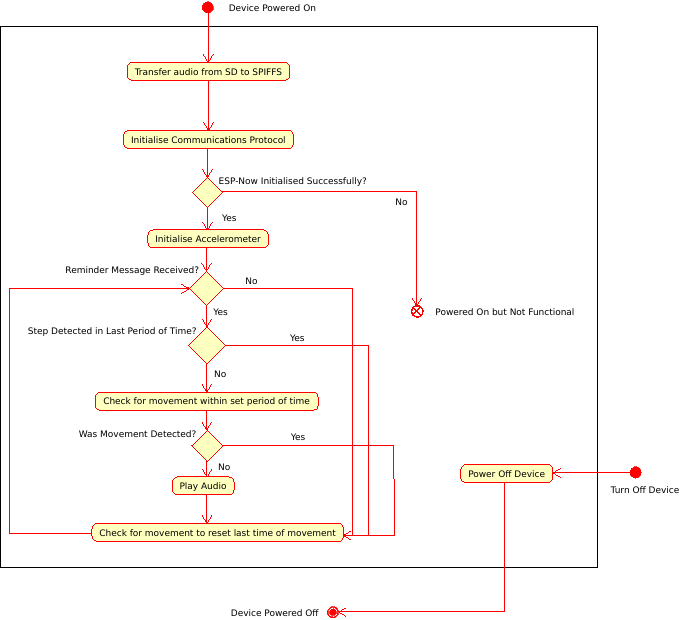
\includegraphics[width=1.0\linewidth]{./UML/WalkingAidDevice/activity diagram.png}

% Caption is defined with a short and long version. The short version is shown in the
% List of Figures section, and the long version is used directly with the figure.
	\caption[Walking Aid Device Activity Diagram]{An activity diagram for the walking aid device software system illustrating the workflow of the system.}

% For figures label should be defined after the caption to ensure proper figure numbering.
	\label{fig:activity_diagram_walking_aid}

\end{figure}
            
                The system begins as soon as the device is powered on. The first process that the system runs is the transferral of the SD audio file to the SPIFFS storage location for quicker access later on. If an error is detected with the process of transferring the audio file from SD card to SPIFFS, then system is left in a non-functional state. The system then attempts to initialise the ESP-Now communication with the wearable device. If this is unsuccessful then it will sit in an inactive state. Otherwise, it will attempt to initialise the accelerometer and begin the loop function of the sketch. 

                For each pass of the loop function, the system firstly checks to see if a reminder message has been received from the wearable device. This message basically states, ``The wearable device is moving, is the walking aid device moving also?''. At this stage, the system checks if the time of the last detected step happened within the last developer set period of time. If a step had been detected in that time, then we skip to the end of the loop and check again for movement in the walking aid to update the last time a movement was detected. Otherwise, we then run a loop for the developer set period of time to check if movement is then detected. This allows the user time to get to their walking aid before having a reminder played or a vibration played through the wearable device. If movement was not detected in that period of time, then we play the audio reminder or send a vibrate message to the wearable device if the user is deaf. If movement was detected then we skip playing the audio or sending a vibrate message and move to the end of the loop. In all instances, the end of the loop signifies that the check for movement should occur again. As previously stated, this is to update the timestamp of the last movement detected. Once this is complete, we move back to the check for reminder message step to start the loop again.

                To terminate the execution of the system prematurely, the device can be powered off. We may not have followed the etiquette of activity diagrams to demonstrate this, but we wanted to demonstrate that the system remains functional in a constant loop unless the device is powered off. We added a second initial activity of turn off device to demonstrate this, where a power off device activity is run and we finish in a state where the device is powered off and non-functional.
            
    \section{Wearable Device}
    \label{sec:wearabledevice}

        The wearable device is one that can be worn on the limbs of the patients to identify when the patient has begun walking. When walking is detected, communication occurs between the walking aid and wearable device to identify if the walking aid device is moving also. 

        \subsection{Walking Detection Technique - Single-Tap Detection}
        \label{subsec:walking_detection_technique}

           With the movement detection of the walking aid device, it was an obvious decision to utilise the single-tap detection feature of the ADXL345 accelerometer. We assume that the walking aid will take the form of a walking stick or Zimmer frame like structure, with movement likely to include lifting and placing. The placing event will cause a change in gravity through the Z-Axis of the accelerometer, and thus will allow the accelerometer to notice a tap being detected.

           The decision of what system to use to detect movement in the wearable device was less simple. Options included using a similar single-tap detection system, a system that utilises changes in acceleration to detect walking, or a system that uses the Bluetooth Low Energy (BLE) technology of each device to measure changes in distances between them. With the option of utilising BLE technology to detect walking, we would have needed to also utilise an accelerometer on one of the devices still to gain an understanding of which device was moving. However, the use of BLE technology for this use case would have been inadequate due to its potential for distance calculation inaccuracies of up to several metres \cite{Fachri_2019}. 

           Therefore, we were left with the utilisation of the ADXL345 accelerometer for the detection of the user walking. To decide on which solution of accelerometer system to use, we decided to develop both the single-tap detection system and the acceleration change detection system and compare them in real world testing. For our system, the single-tap detection system seemed to work better in attempting to detect walking, where the system attempting to detect changes in acceleration struggled with also detecting any movements in the accelerometer. The single-tap detection system would also be beneficial to us as it would be implementable on both the walking aid and wearable devices. Another benefit to the single-tap detection solution is that it allows versatility as to where the wearable device can be placed, with testing proving that the devices can detect walking on both the user's wrist and their ankle. 

           Ultimately, we decided to implement the single-tap detection system within the wearable device to detect when the user was walking. We make use of a system that checks if the user makes 5 steps within a 10-second period in order to meet the user requirement of reminders only being played if the user has moved over a metre without their walking aid. If they do, then we send a message to the walking aid device to play an audio reminder to the patient to take their walking aid with them if the walking aid device has not detected movement. The main benefits to this system is its versatility to be worn on the user's wrist or ankle, and it provided the foundations to the similar system that has been developed for the walking aid device. In future, we would like to explore the use of the aforementioned ultra-wideband technology (UWB). Due to its distance measurement error b
           eing within 10 cm \cite{uwb_accuracy}, it would have been interesting to implement this within the wearable device, and into the walking aid device working in conjunction with an accelerometer to detect if the walking aid is moving.

        \subsection{Physical Design}
        \label{subsec:Design_Decisions_wearable}
            As with the walking aid device, the design was formulated around a minimalistic form factor around the components that needed to be present, in this case, the TinyPico, ADXL, and vibration motor. This prototype needed to be of a particularly small form factor; the client made it clear that patients aren't always happy with new, large and obtrusive objects on their bodies, so the more natural we could make it, the better it would be. This device is very tightly packed, with the components in very short distances of one another, although this could be an issue with electrical shorts, during assembly there will be insulating factors included, that will stop this from happening.

            \begin{figure}[H]
\centering
\begin{minipage}{.5\textwidth}
  \centering
  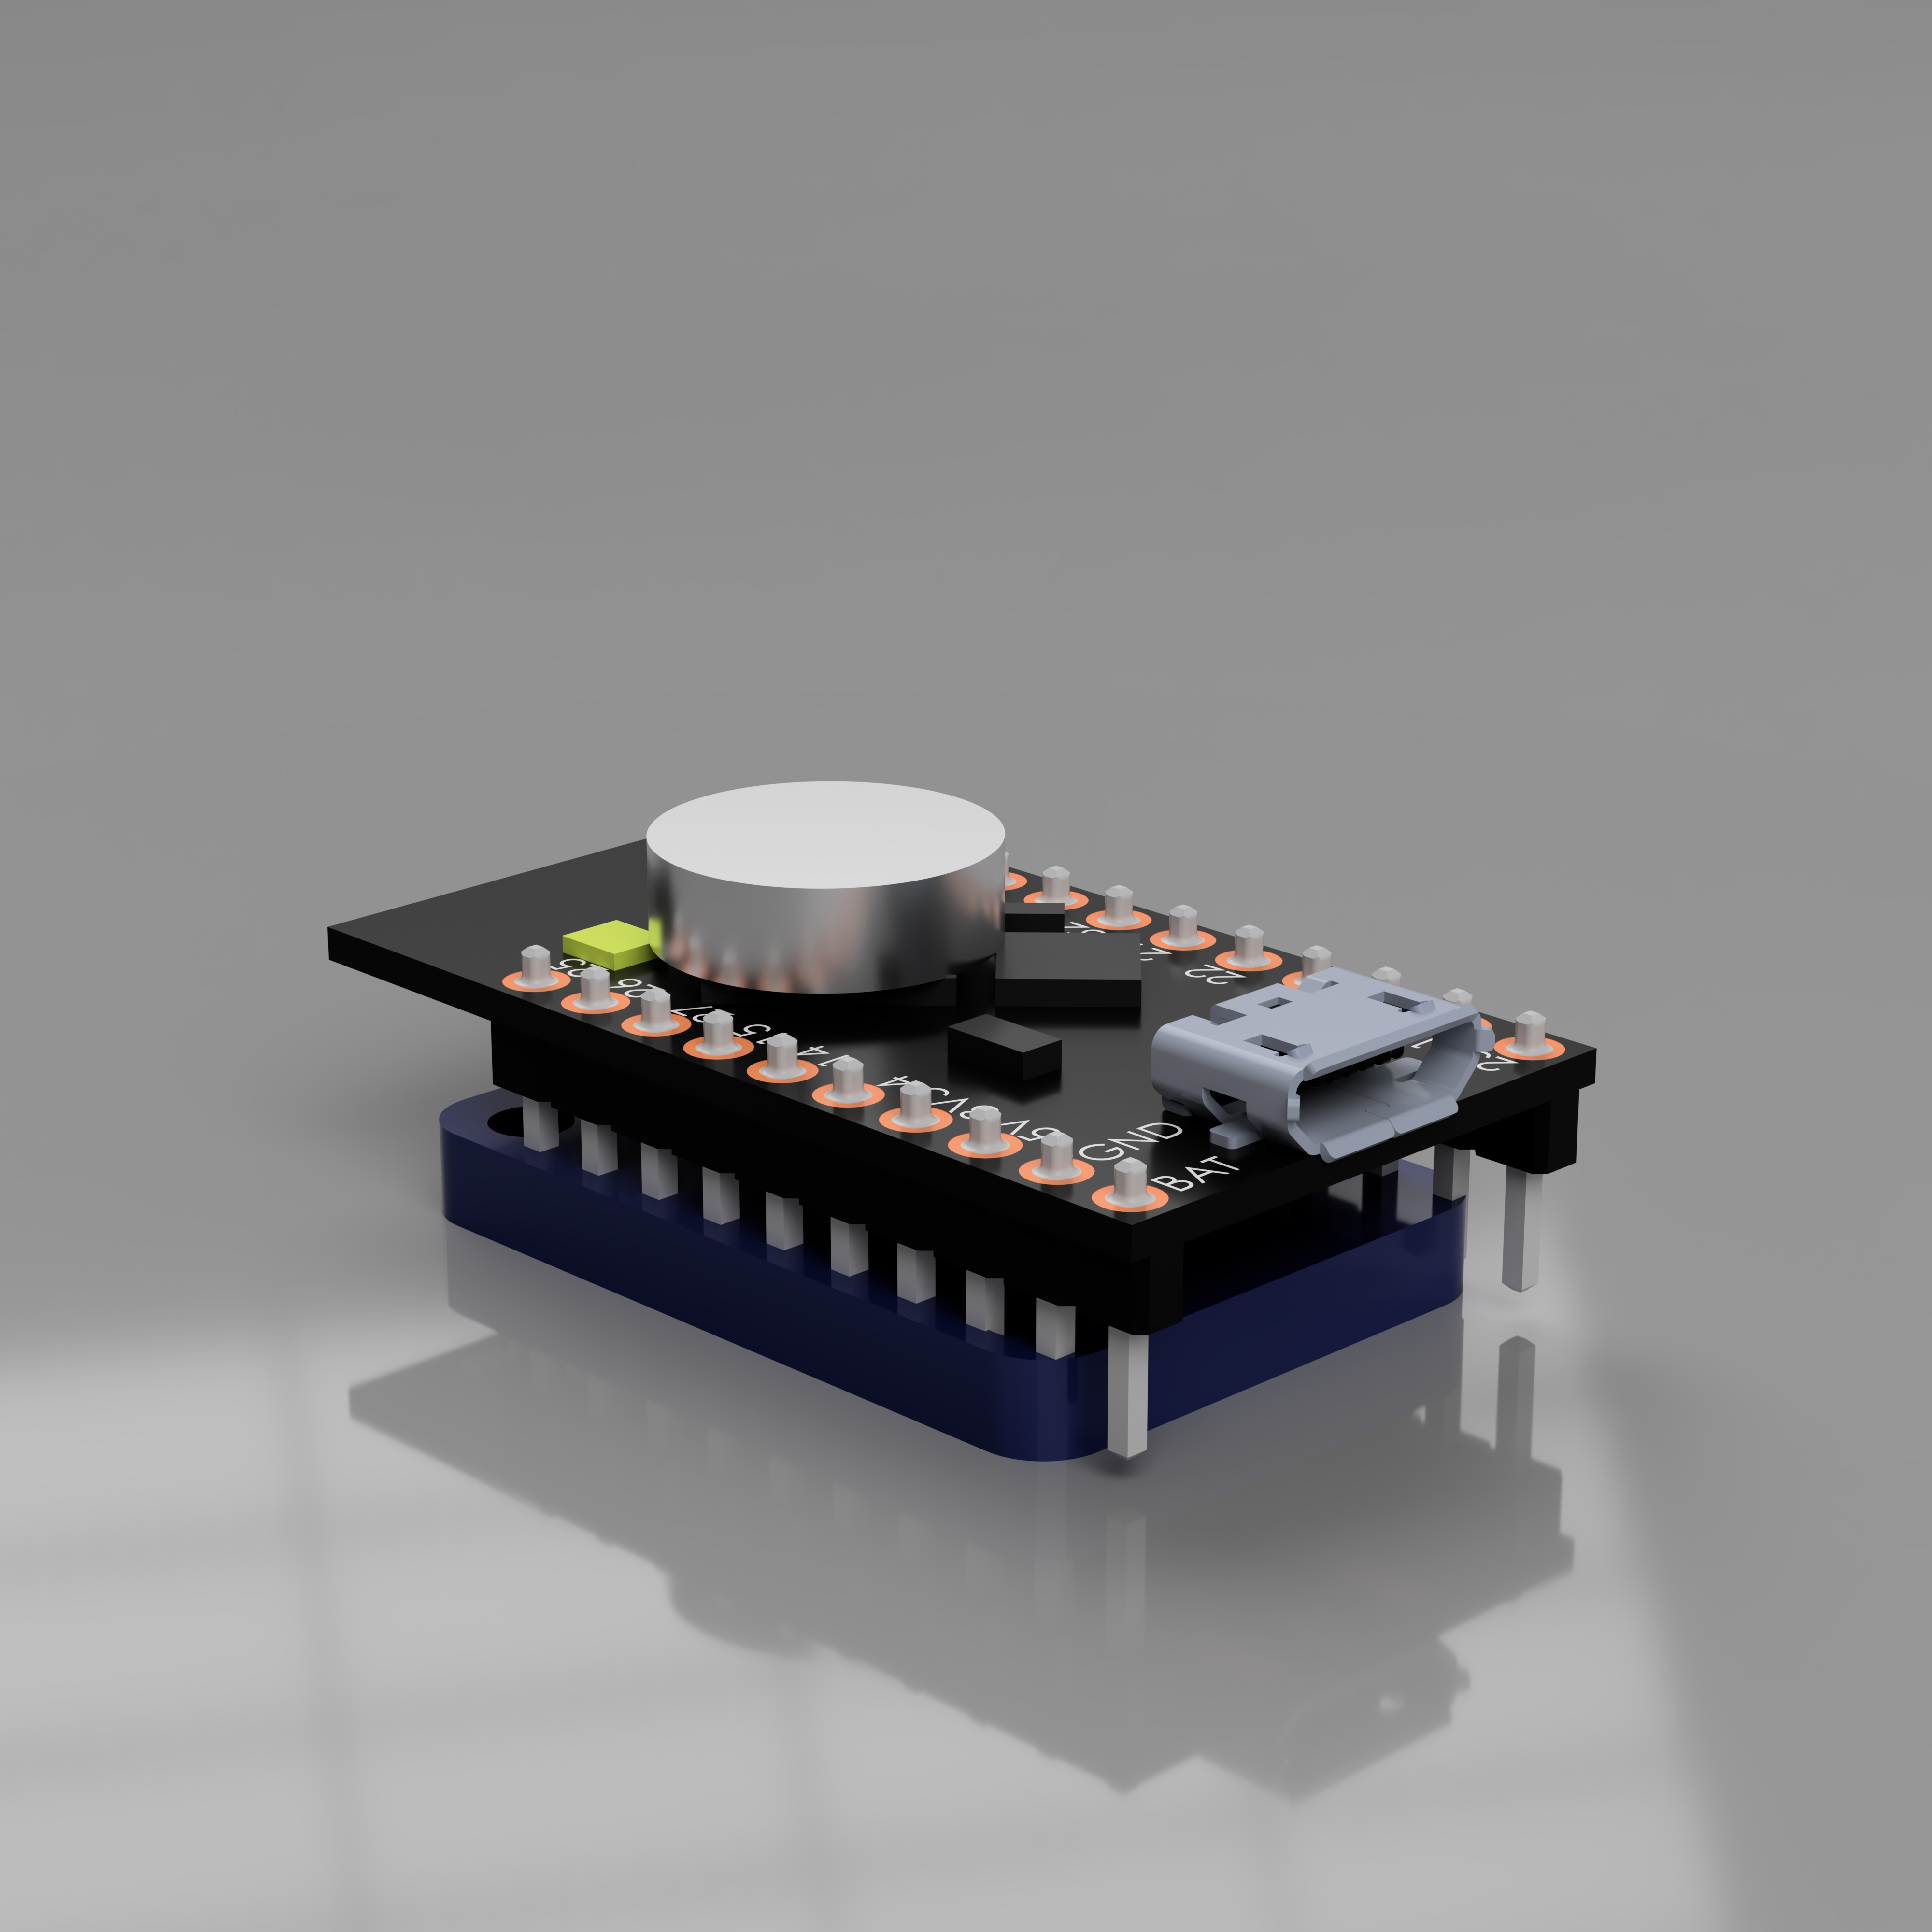
\includegraphics[width=.8\linewidth]{graphics/cad/wearable_components_1.png}
  \captionsetup{width=0.8\linewidth, justification=centering}
  \centering
  \captionof{figure}{Wearable device component layout}
  \label{fig:wearable_components_1}
\end{minipage}%
\begin{minipage}{.5\textwidth}
  \centering
  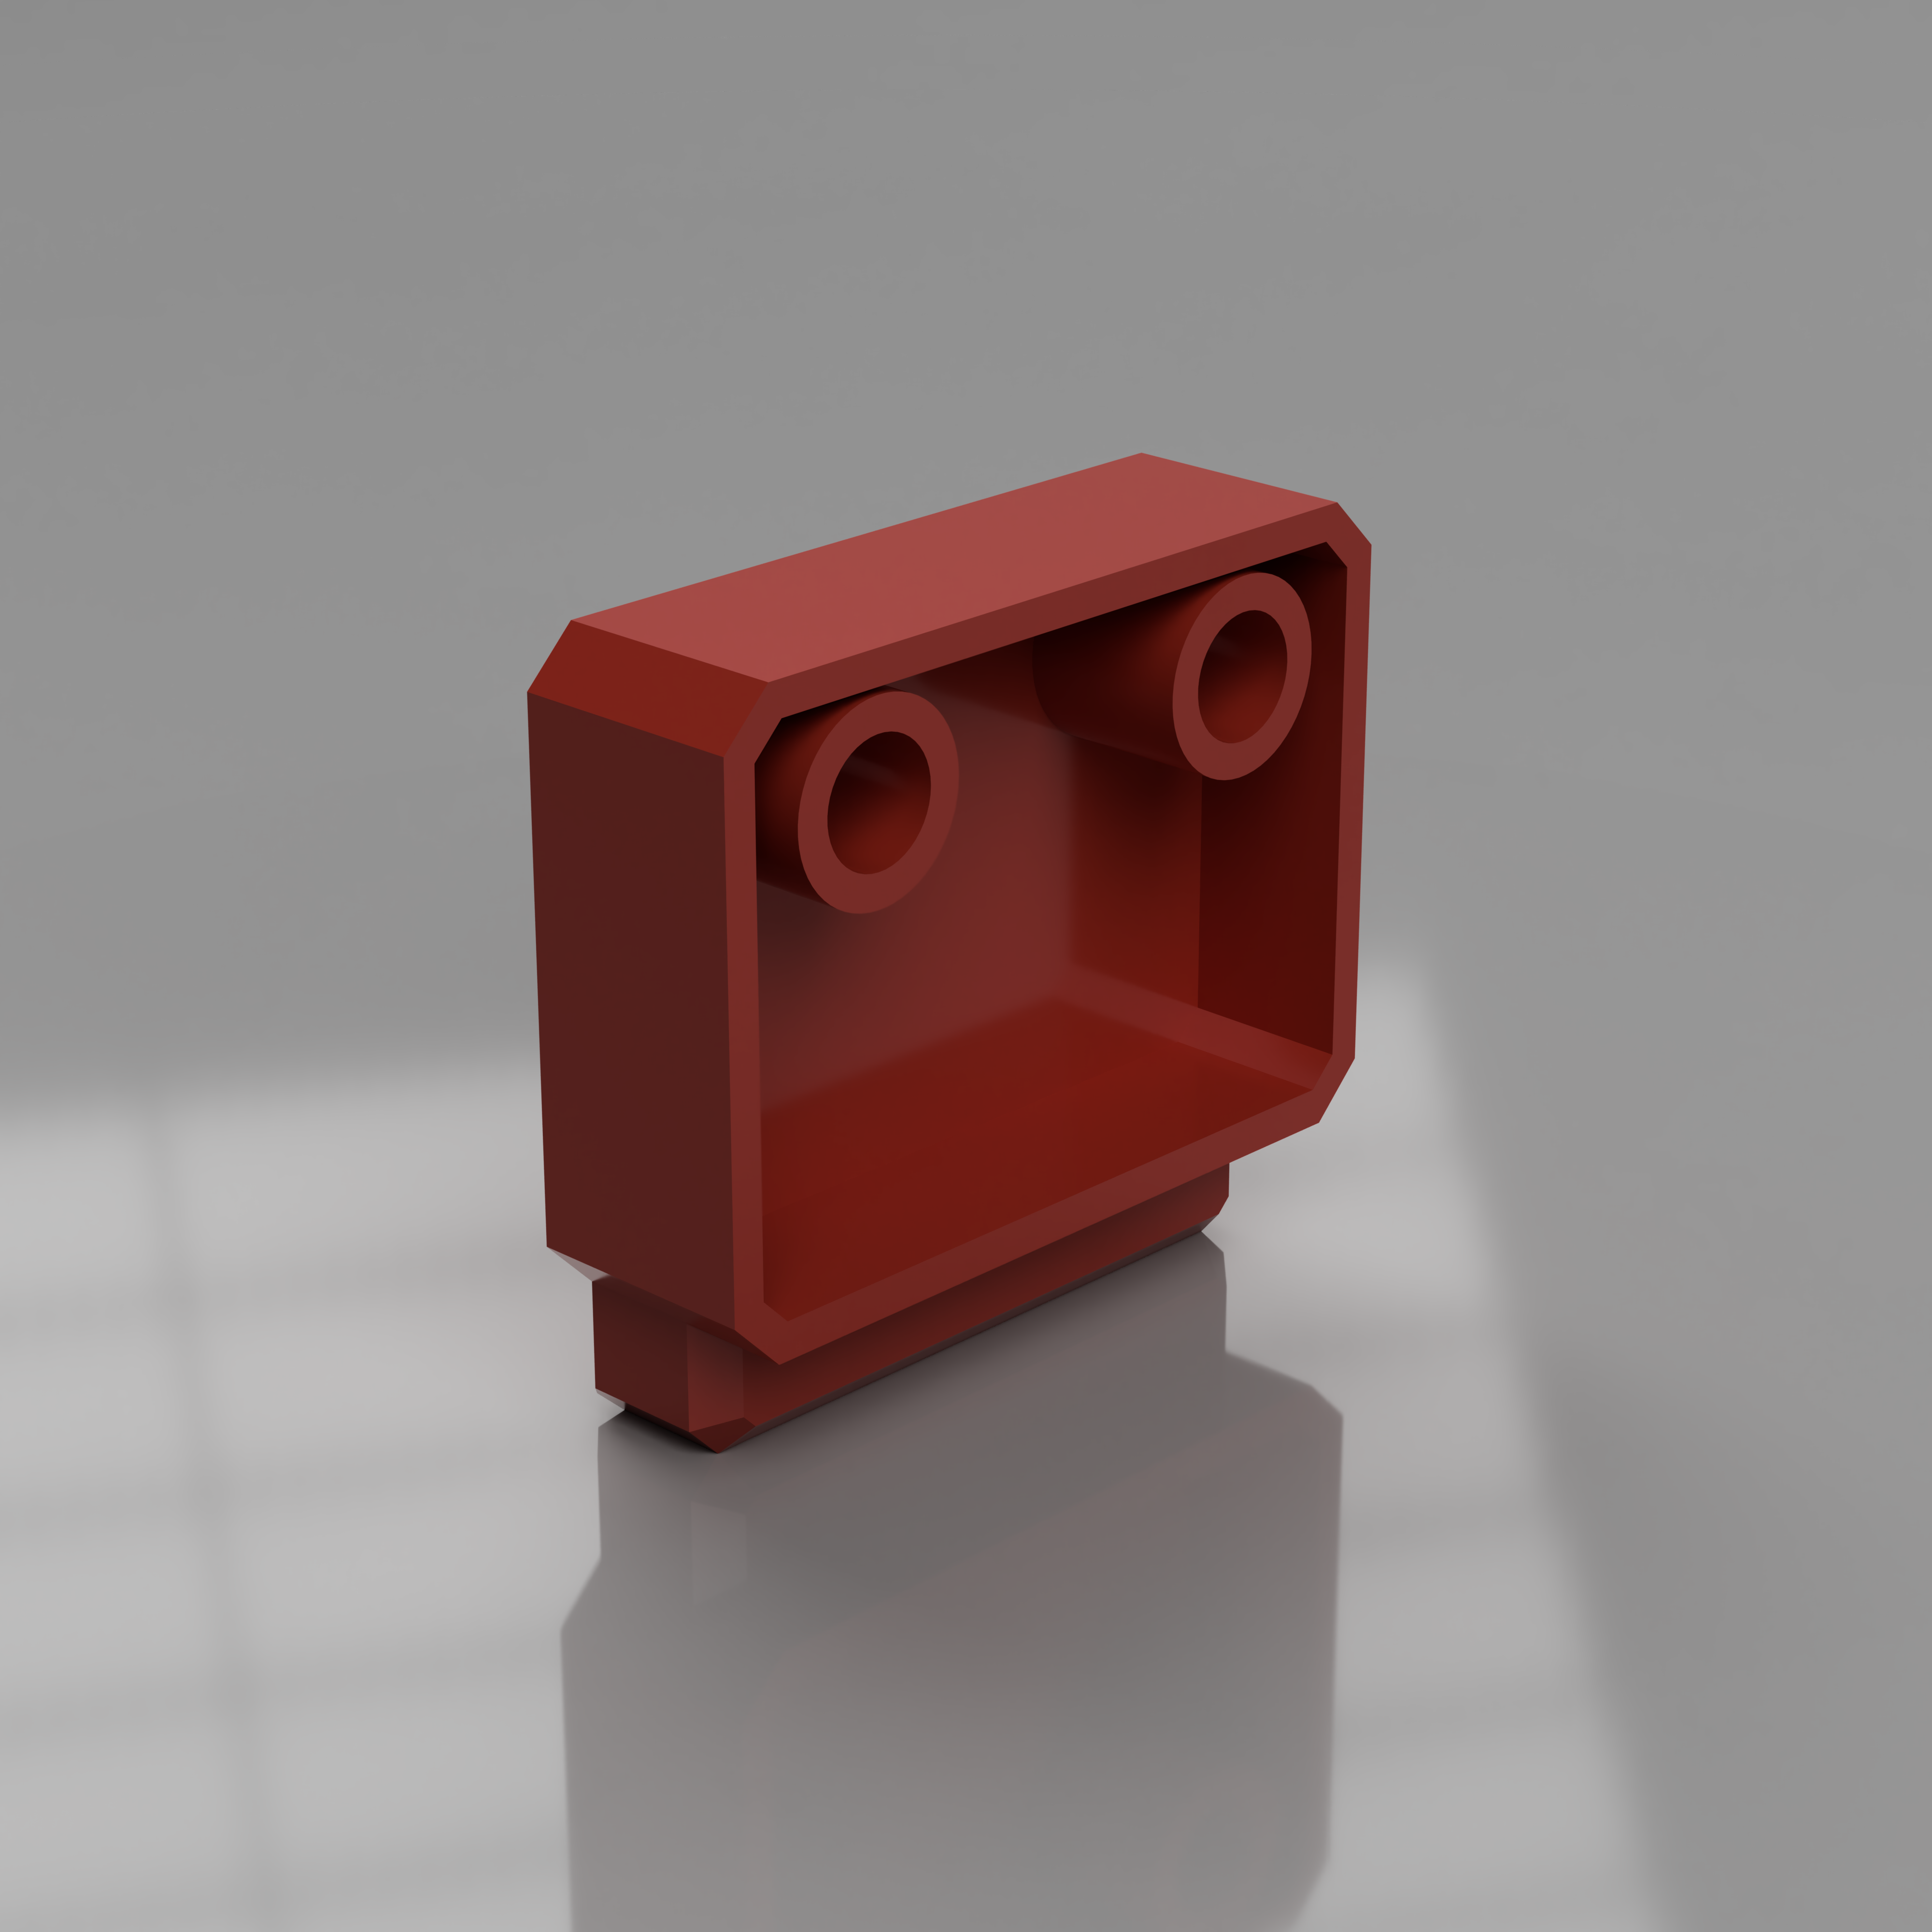
\includegraphics[width=.8\linewidth]{graphics/cad/wearable_endcase_1.png}
  \captionsetup{width=0.8\linewidth, justification=centering}
  \centering
  \captionof{figure}{Walking aid modular end casing}
  \label{fig:walkingaid_endcase_1}
\end{minipage}
\end{figure} %%also includes endcase

            A similar approach was taken regarding the modular design, with an end-housing that can be quickly and easily changed. We designed a base end-plate from which all attachments are based off of, and will include it in the deliverables to ensure the client can adjust and create more as needed from our working template.

            \begin{figure}[H]
\centering
\begin{minipage}{.5\textwidth}
  \centering
  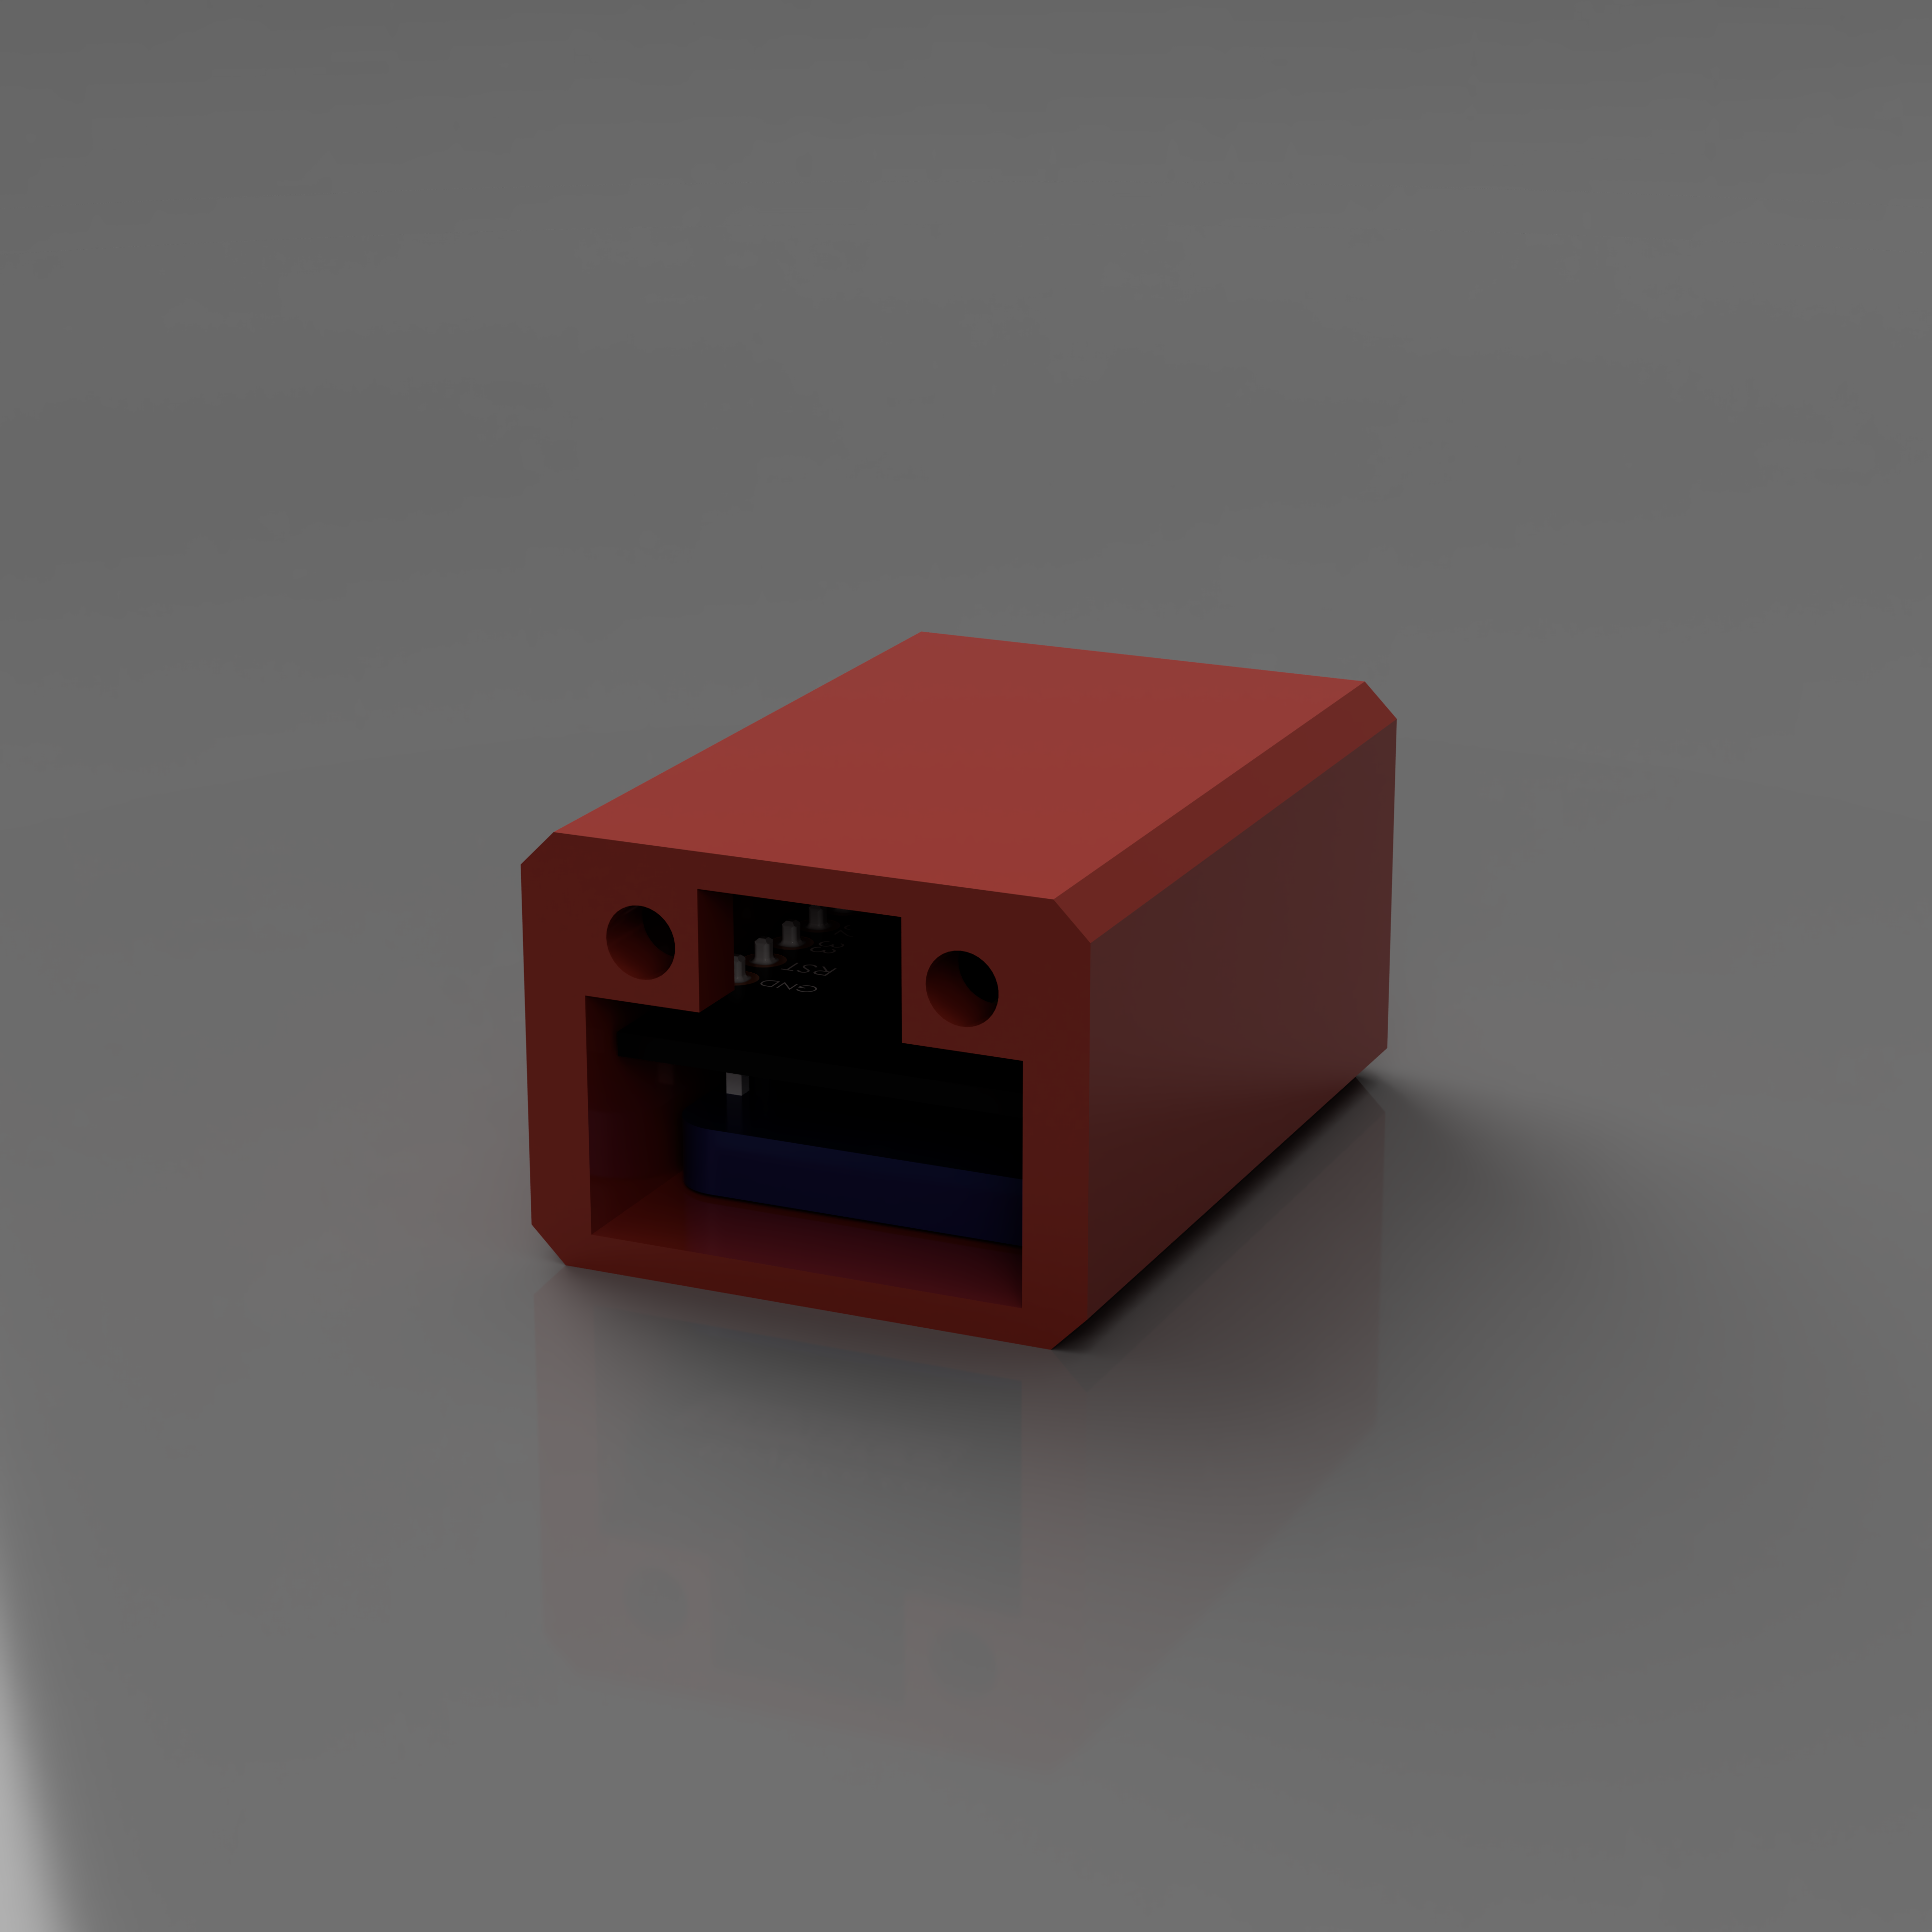
\includegraphics[width=.8\linewidth]{graphics/cad/wearable_2.png}
  \captionsetup{width=0.8\linewidth, justification=centering}
  \centering
  \captionof{figure}{Assembled wearable device}
  \label{fig:wearable_2}
\end{minipage}%
\begin{minipage}{.5\textwidth}
  \centering
  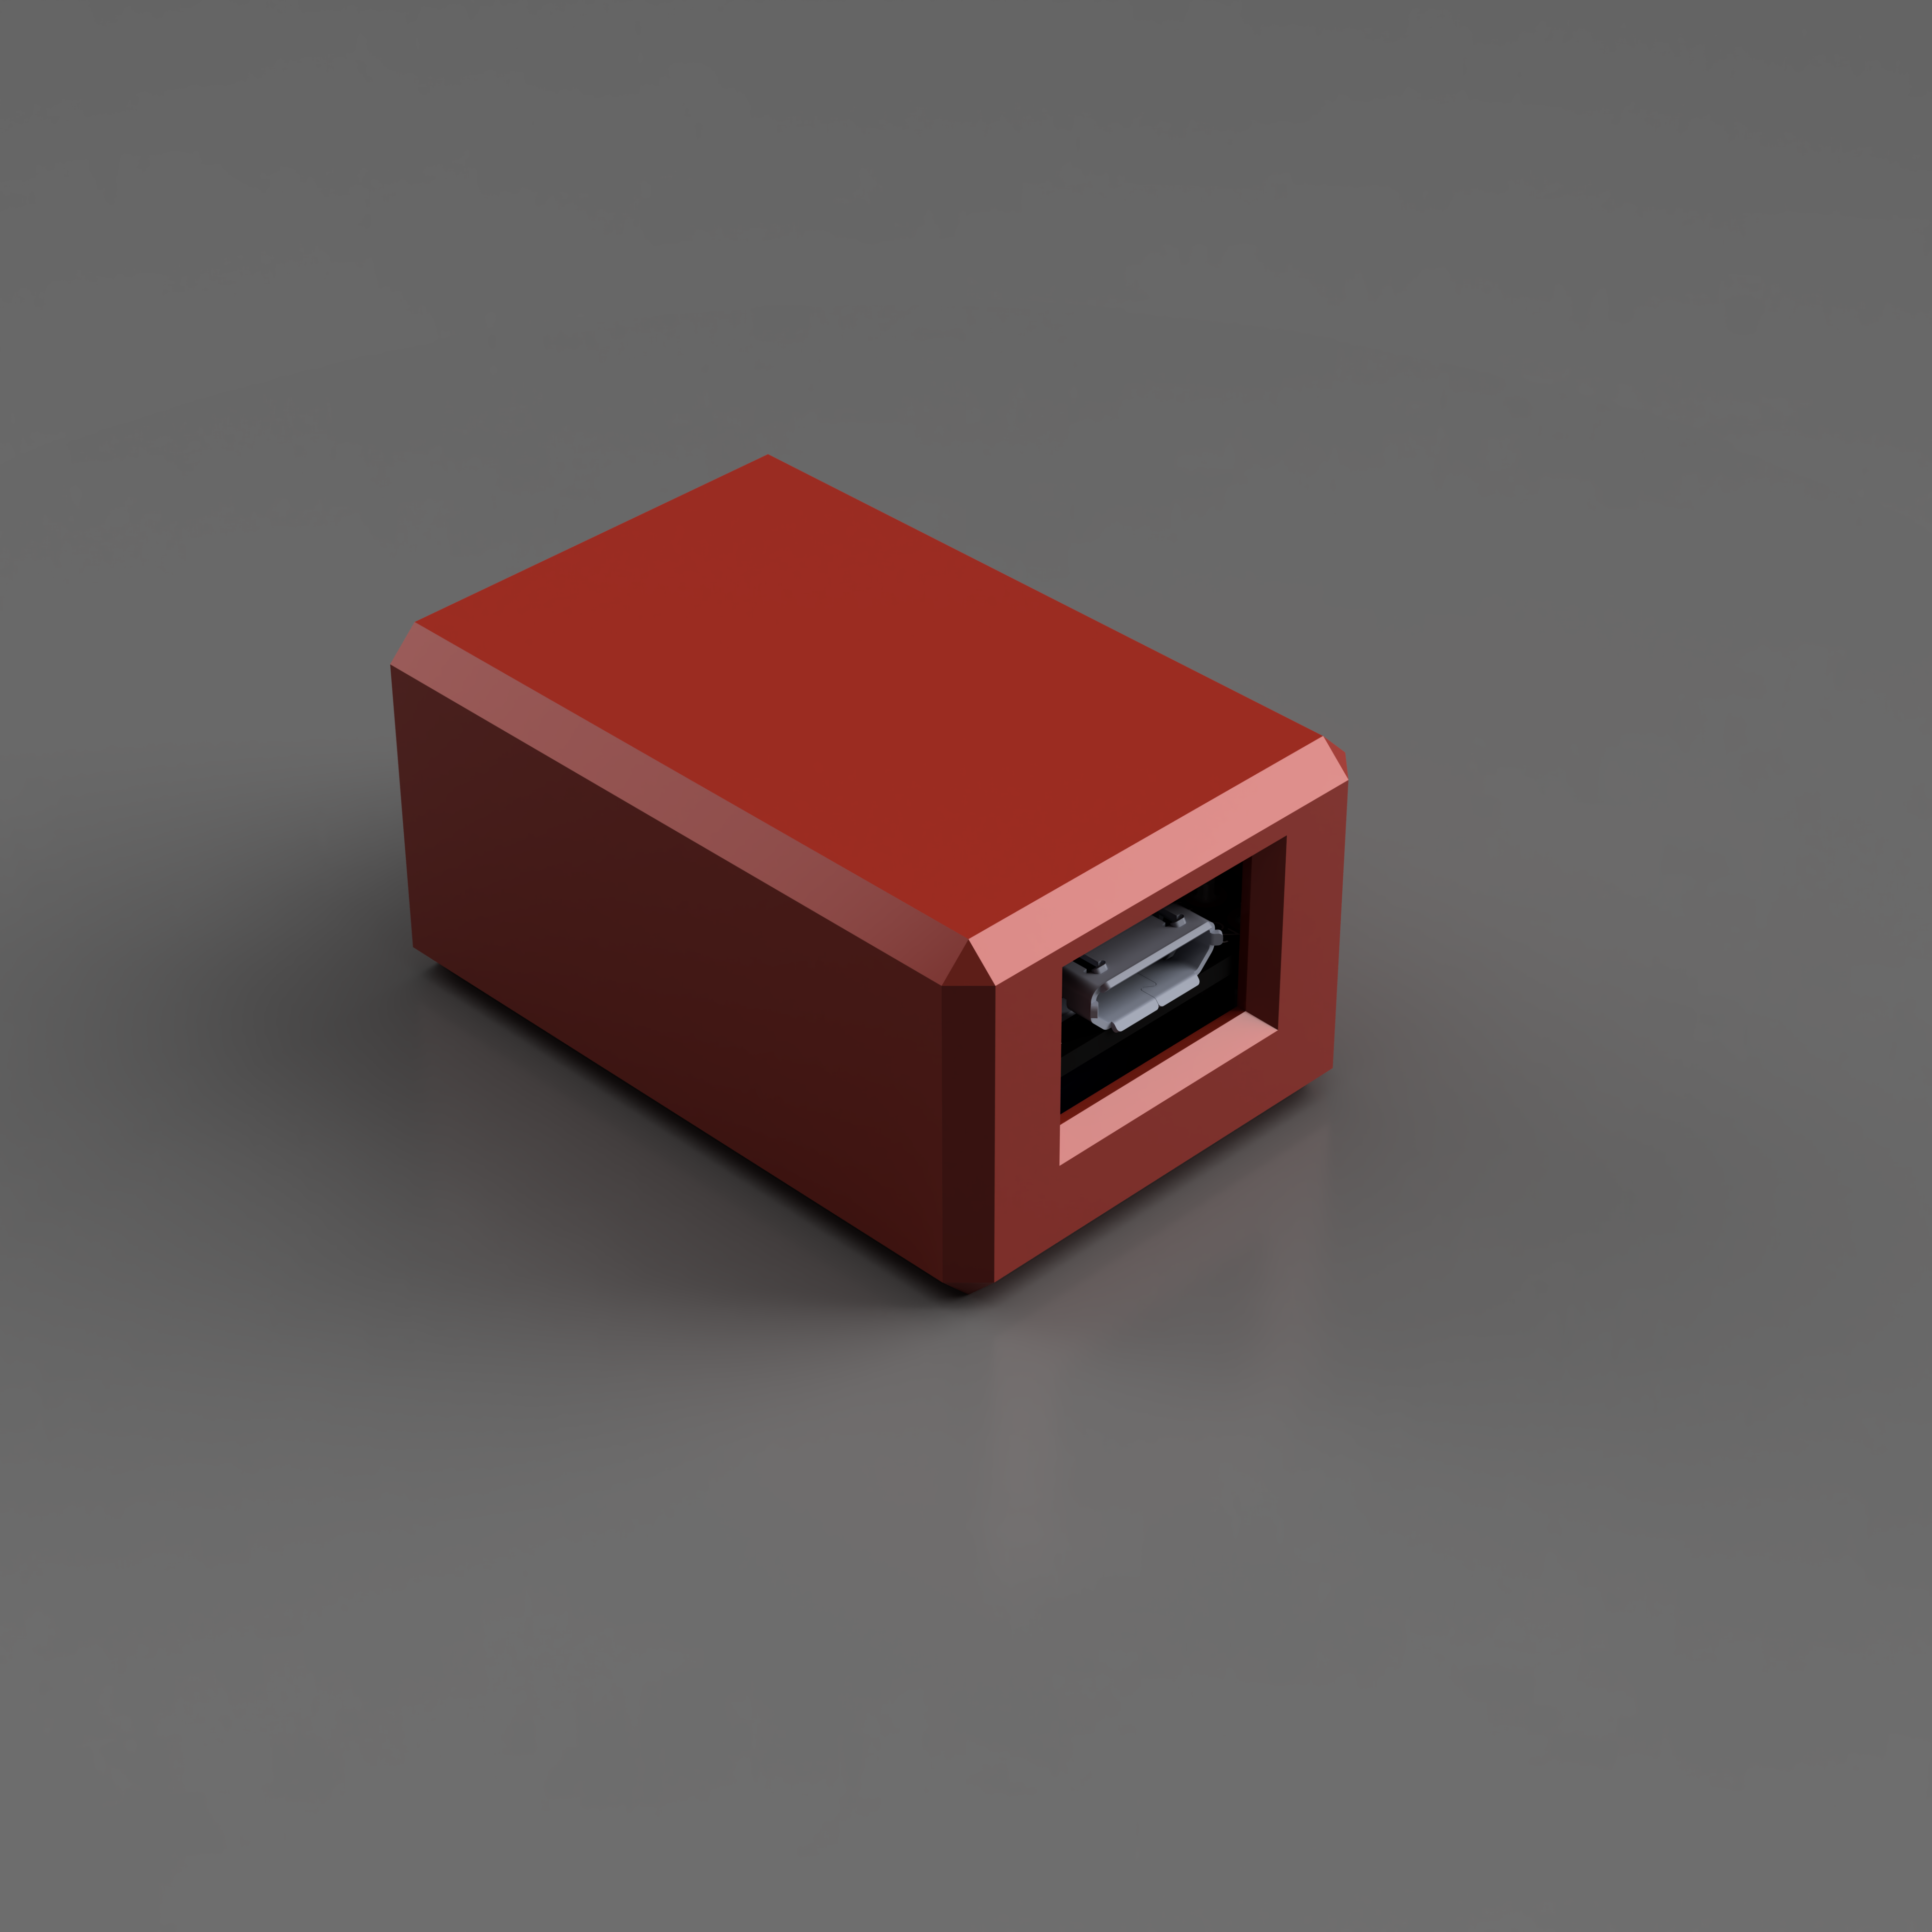
\includegraphics[width=.8\linewidth]{graphics/cad/wearable_1.png}
  \captionsetup{width=0.8\linewidth, justification=centering}
  \centering
  \captionof{figure}{Assembled wearable device}
  \label{fig:wearable_1}
\end{minipage}
\end{figure}

            We have designed and printed two different mounting options to begin with, the first being a "clip on" style attachment, that allows the wearable device to be clipped into pockets, clothing, or existing bands or straps the user may be wearing. This was designed to be a tight, friction fit between the casing and the clip, to ensure there is less chance of the item becoming loose over time.

            \begin{figure}[H]
\centering
\begin{minipage}{.5\textwidth}
  \centering
  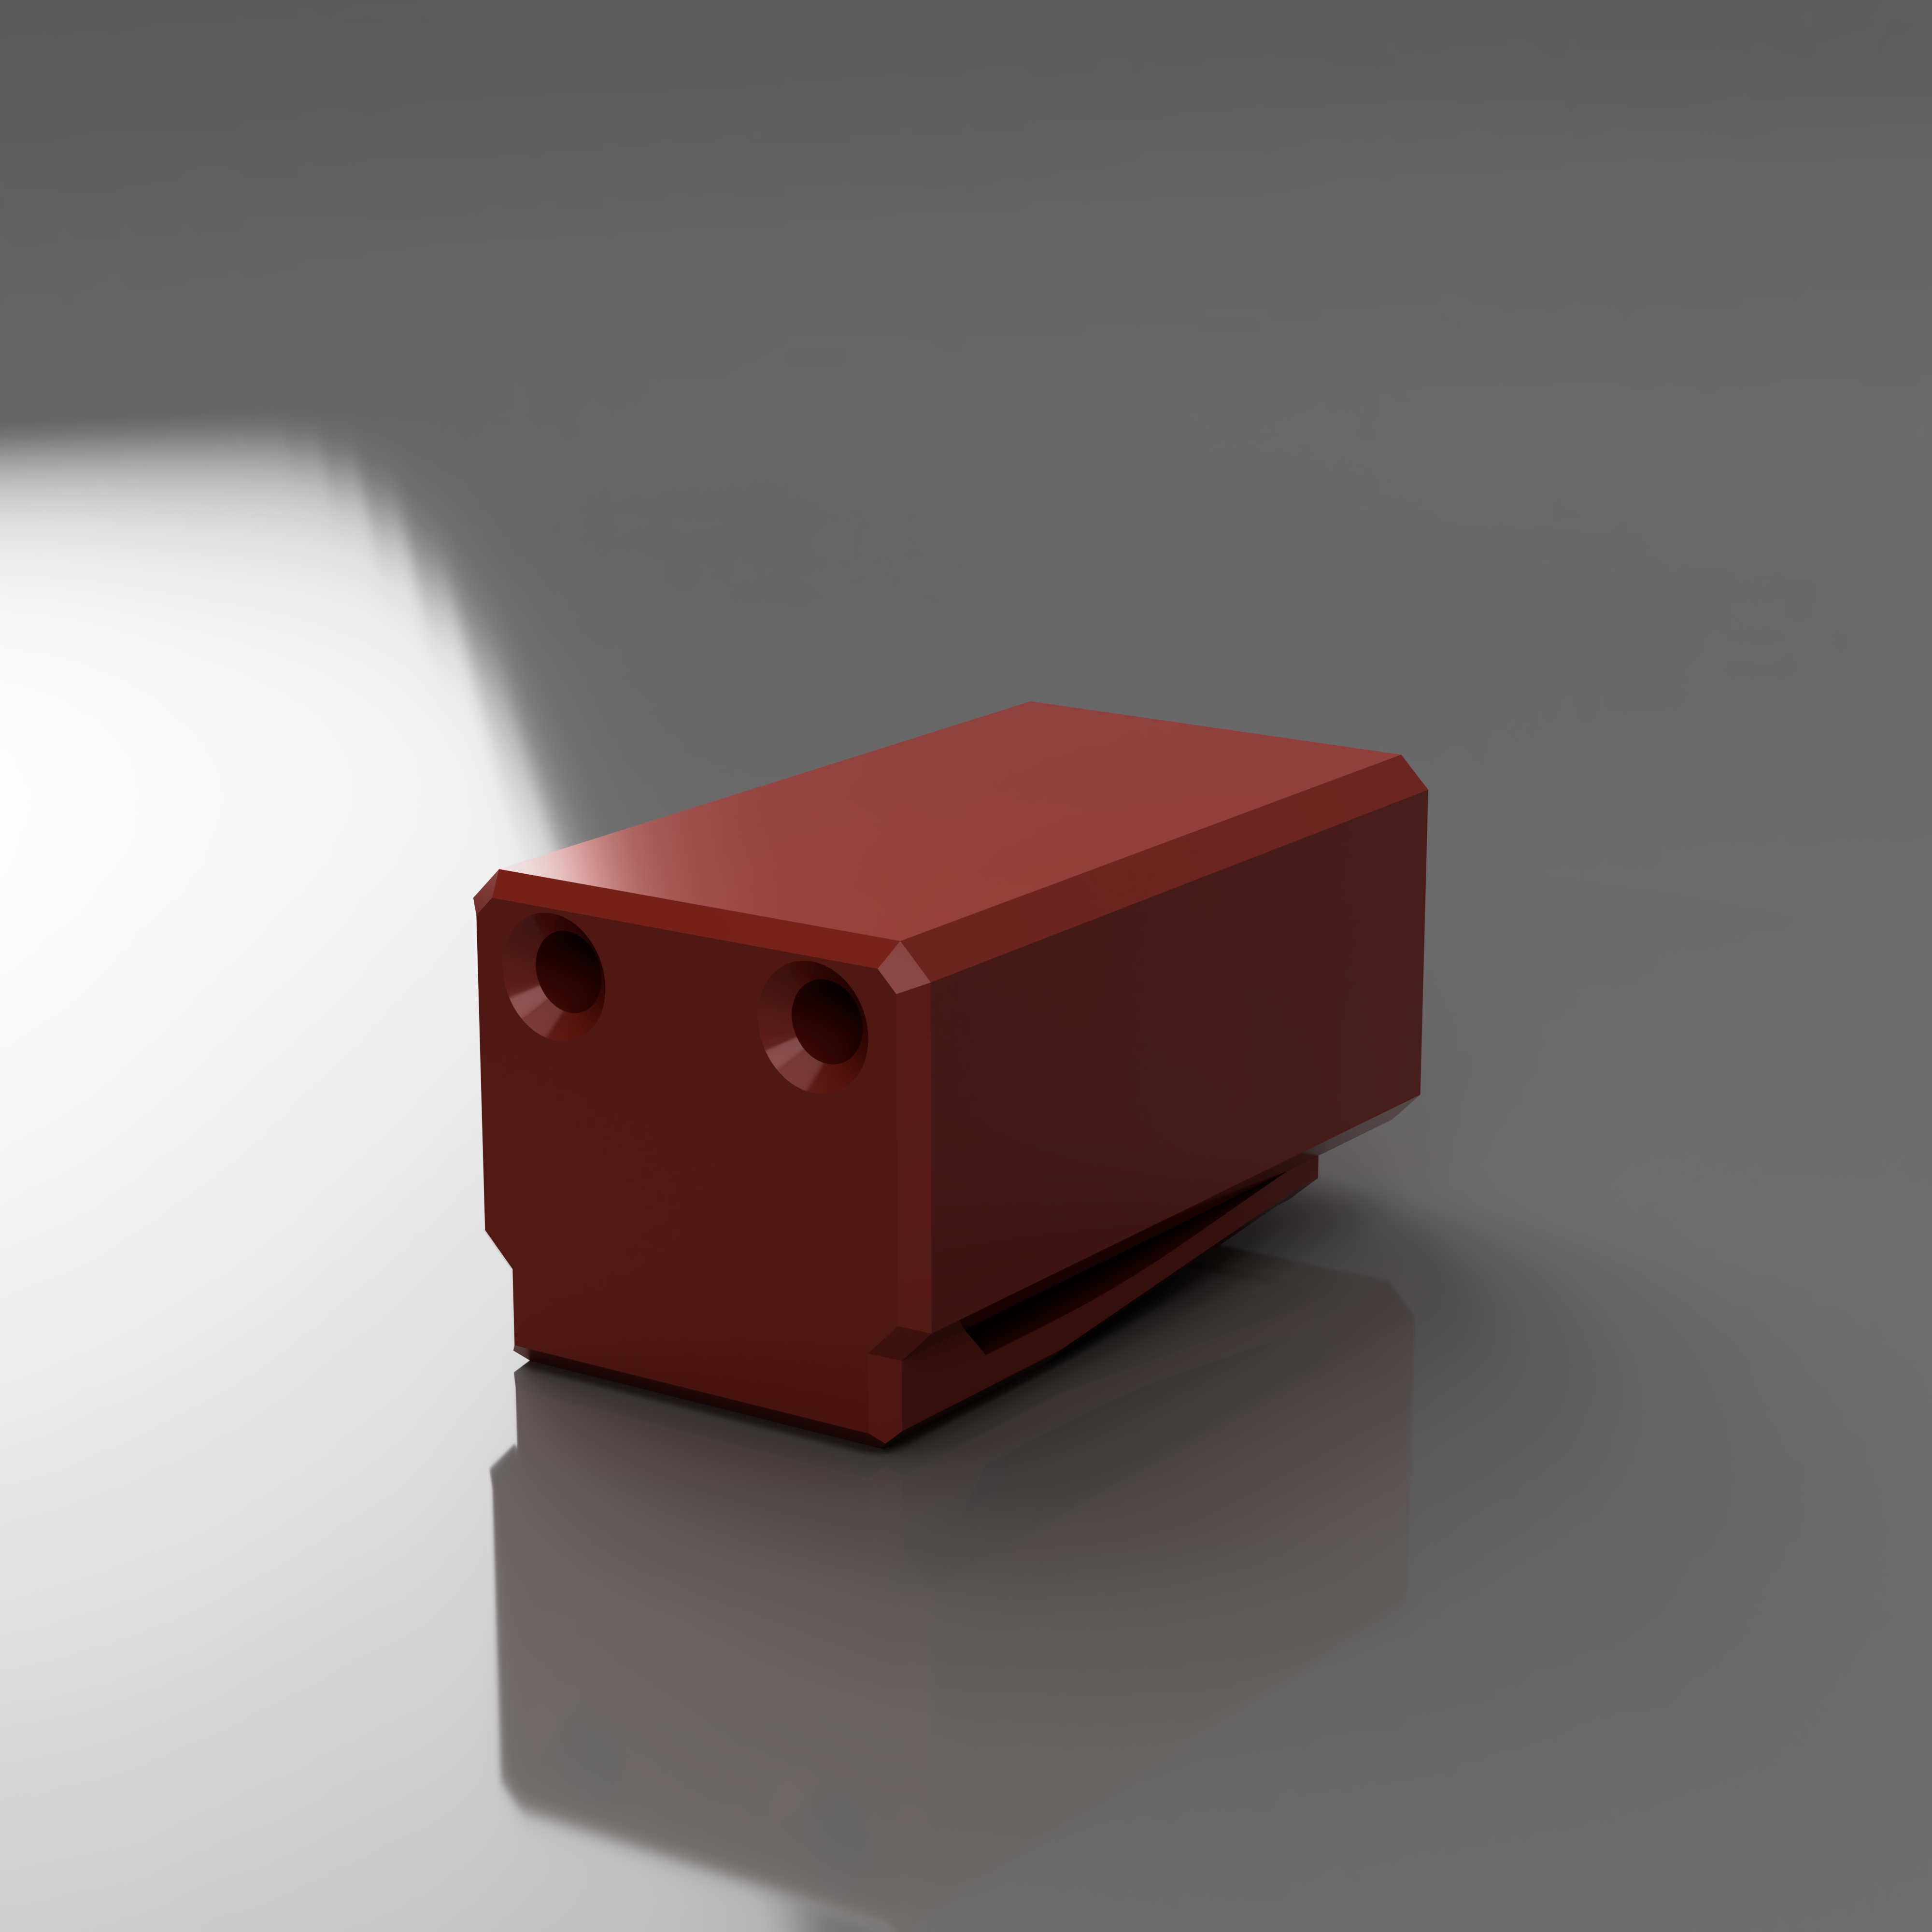
\includegraphics[width=.8\linewidth]{graphics/cad/wearable_clip_1.png}
  \captionsetup{width=0.8\linewidth, justification=centering}
  \centering
  \captionof{figure}{Wearable device with clip attachment}
  \label{fig:wearable_clip_1}
\end{minipage}%
\begin{minipage}{.5\textwidth}
  \centering
  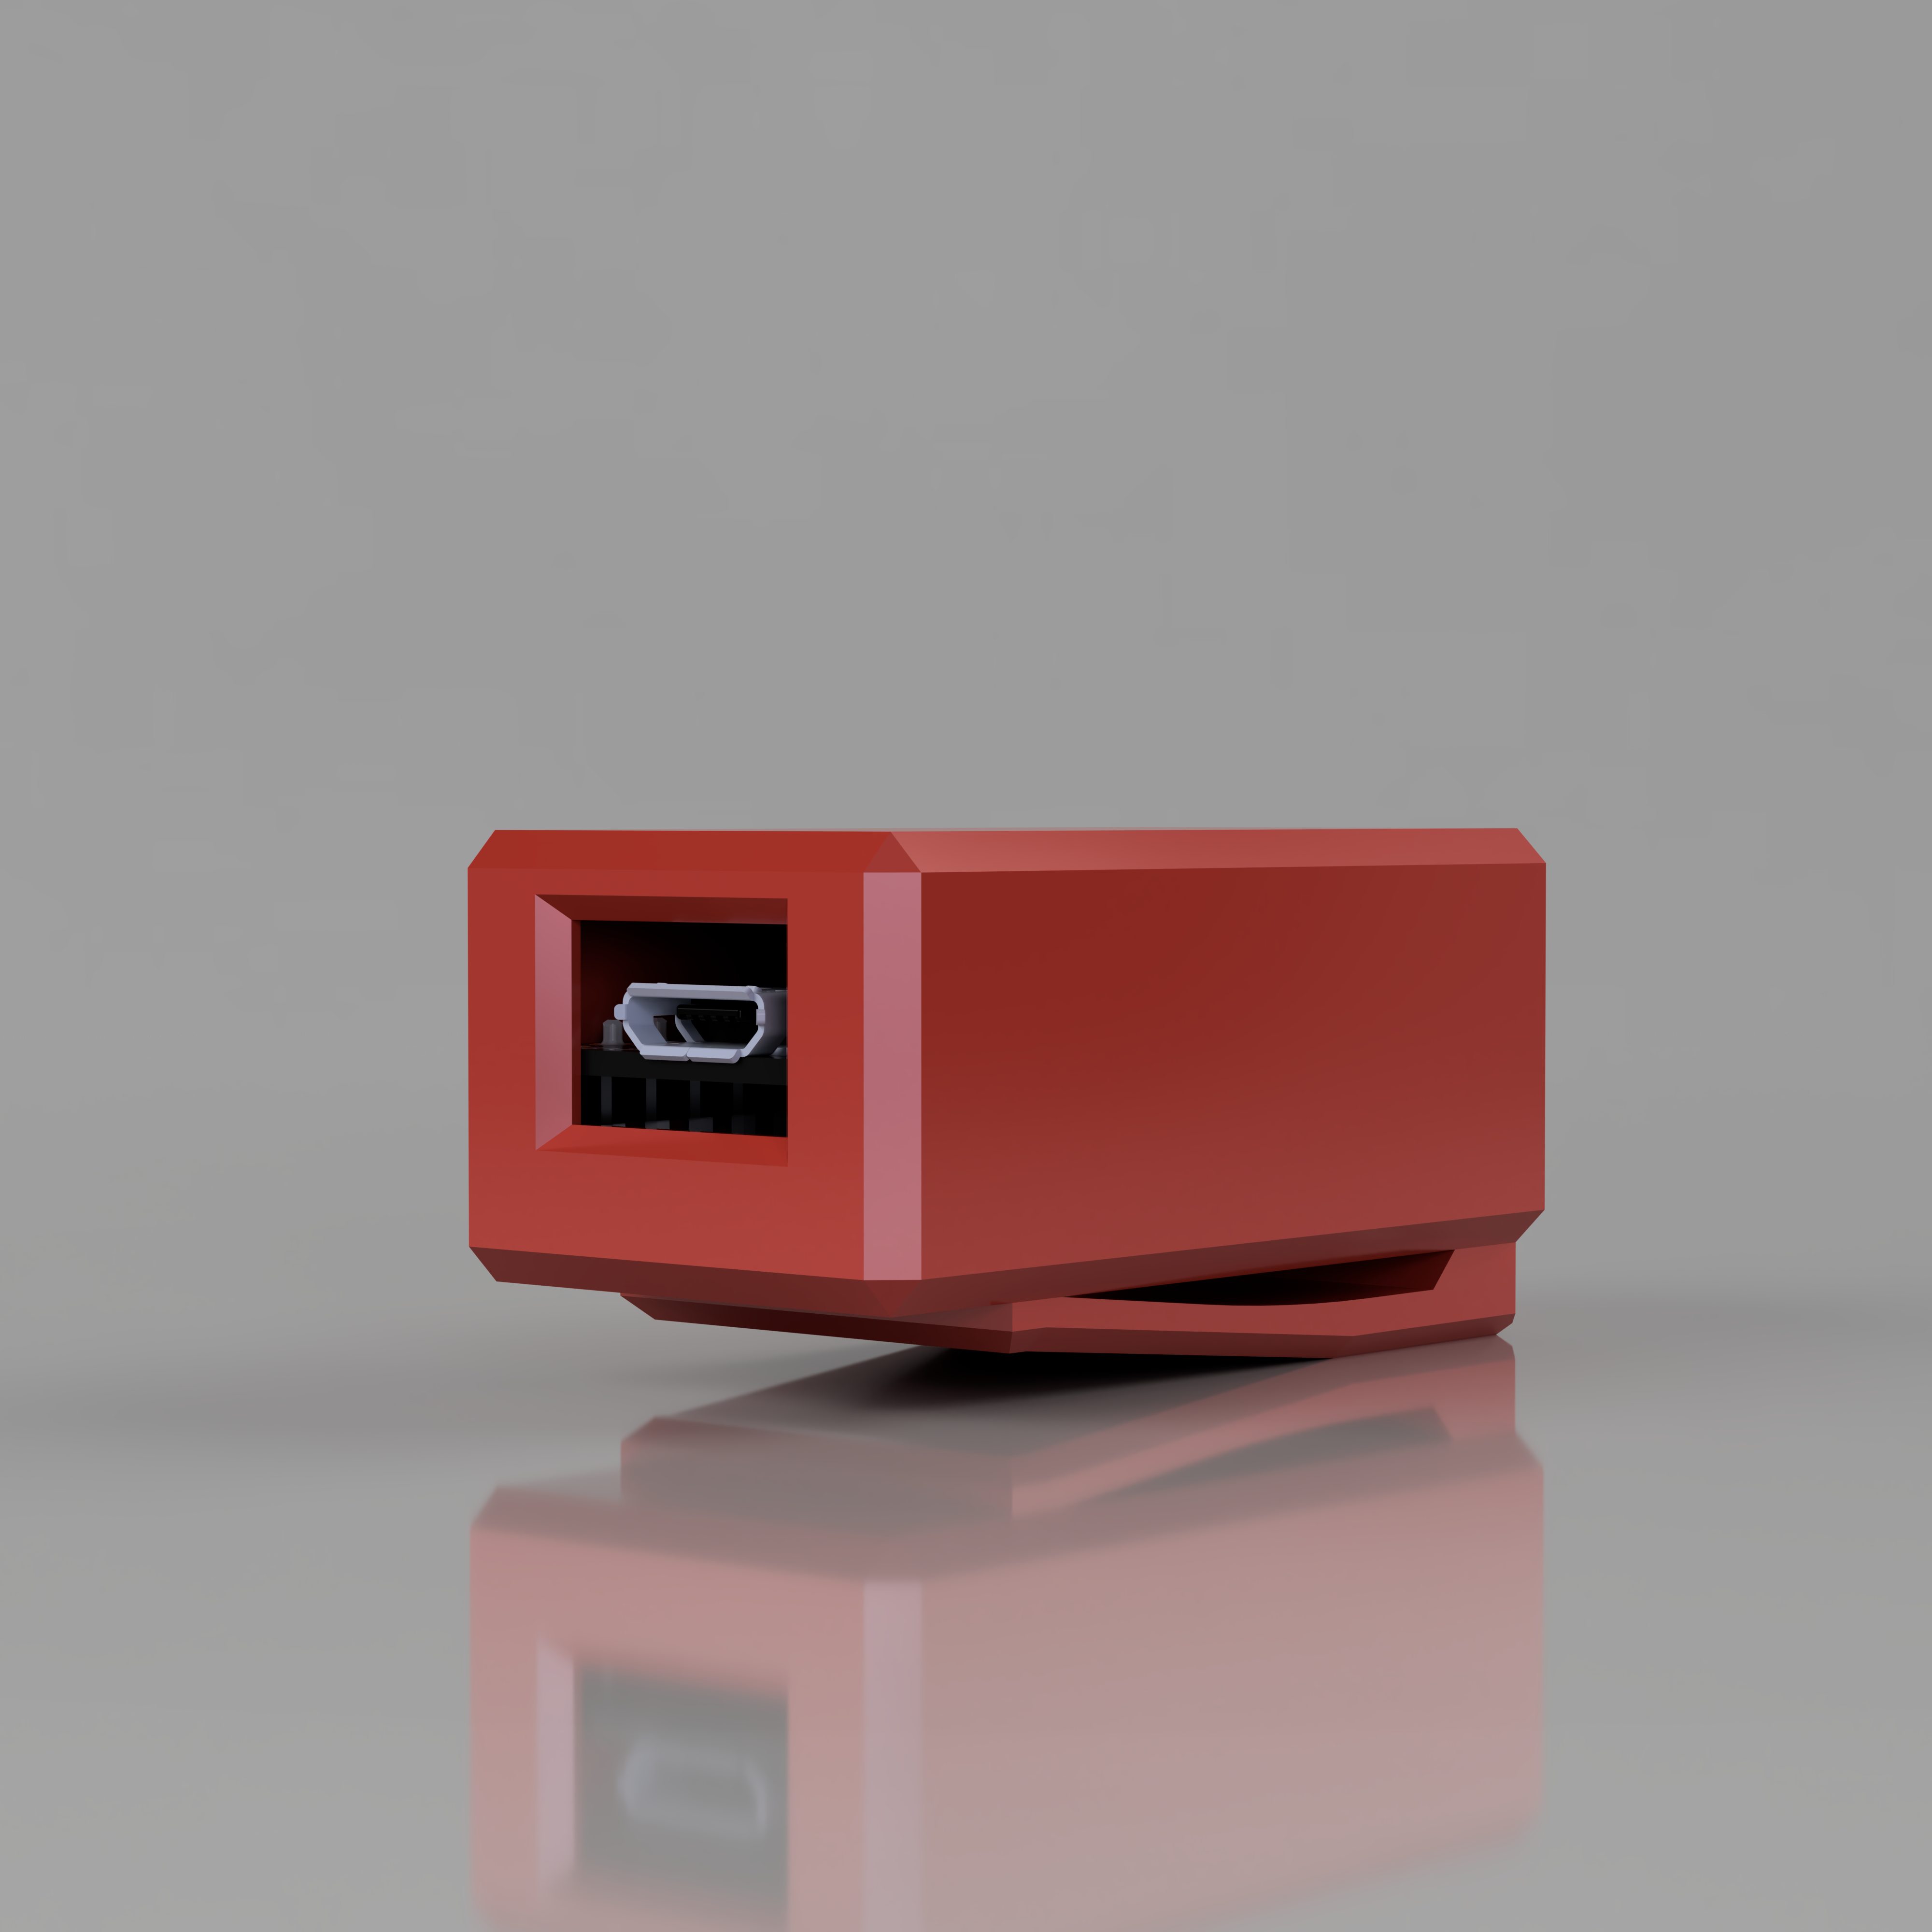
\includegraphics[width=.8\linewidth]{graphics/cad/wearable_clip_2.png}
  \captionsetup{width=0.8\linewidth, justification=centering}
  \centering
  \captionof{figure}{Wearable device with clip attachment}
  \label{fig:wearable_clip_2}
\end{minipage}
\end{figure}

            The second attachment option is a watch strap mount. This allows the wearable device to be used with any standard 22mm watchstrap, and the idea behind this is to allow for a more comfortable, and familiar feel on the arm. Patients aren't always happy trying new things due to their condition, but this should allow for existing watch straps to be used, and making them feel at home with their new device.

            \todo Add IRL pictures

            \begin{figure}[H]
\centering
\begin{minipage}{.5\textwidth}
  \centering
  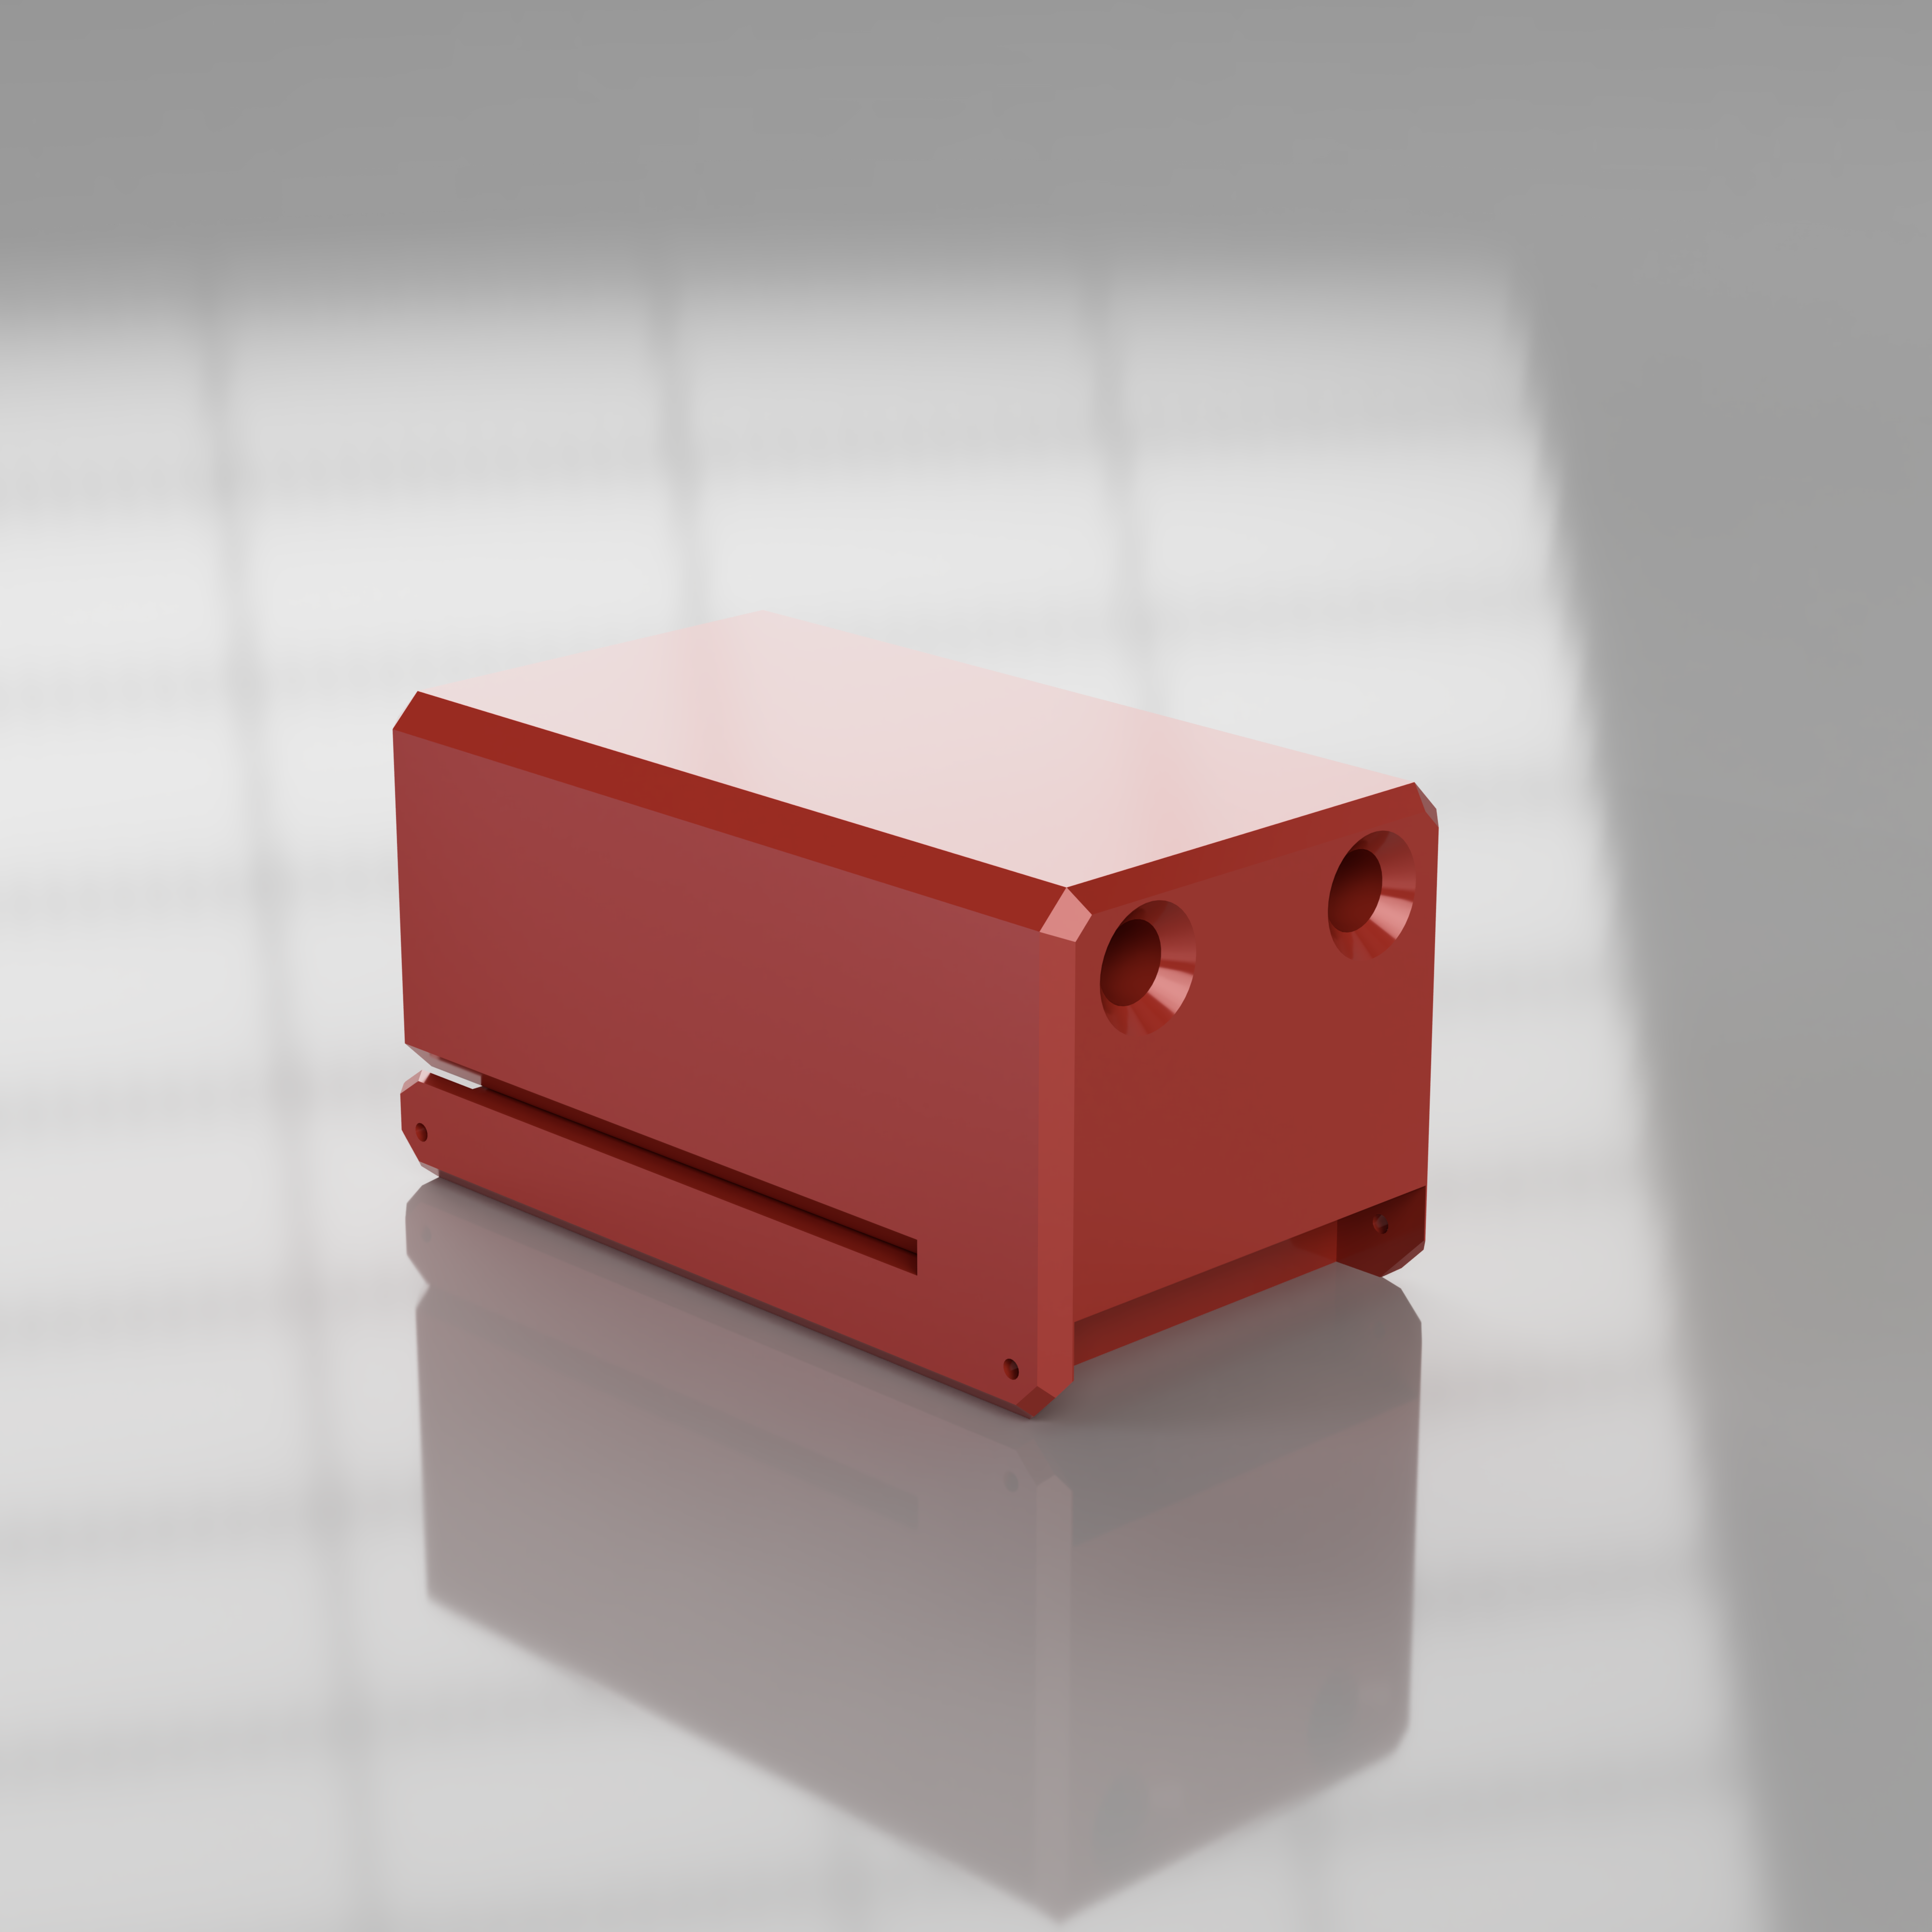
\includegraphics[width=.8\linewidth]{graphics/cad/wearable_strap_1.png}
  \captionsetup{width=0.8\linewidth, justification=centering}
  \centering
  \captionof{figure}{Wearable device with strap attachment}
  \label{fig:wearable_strap_1}
\end{minipage}%
\begin{minipage}{.5\textwidth}
  \centering
  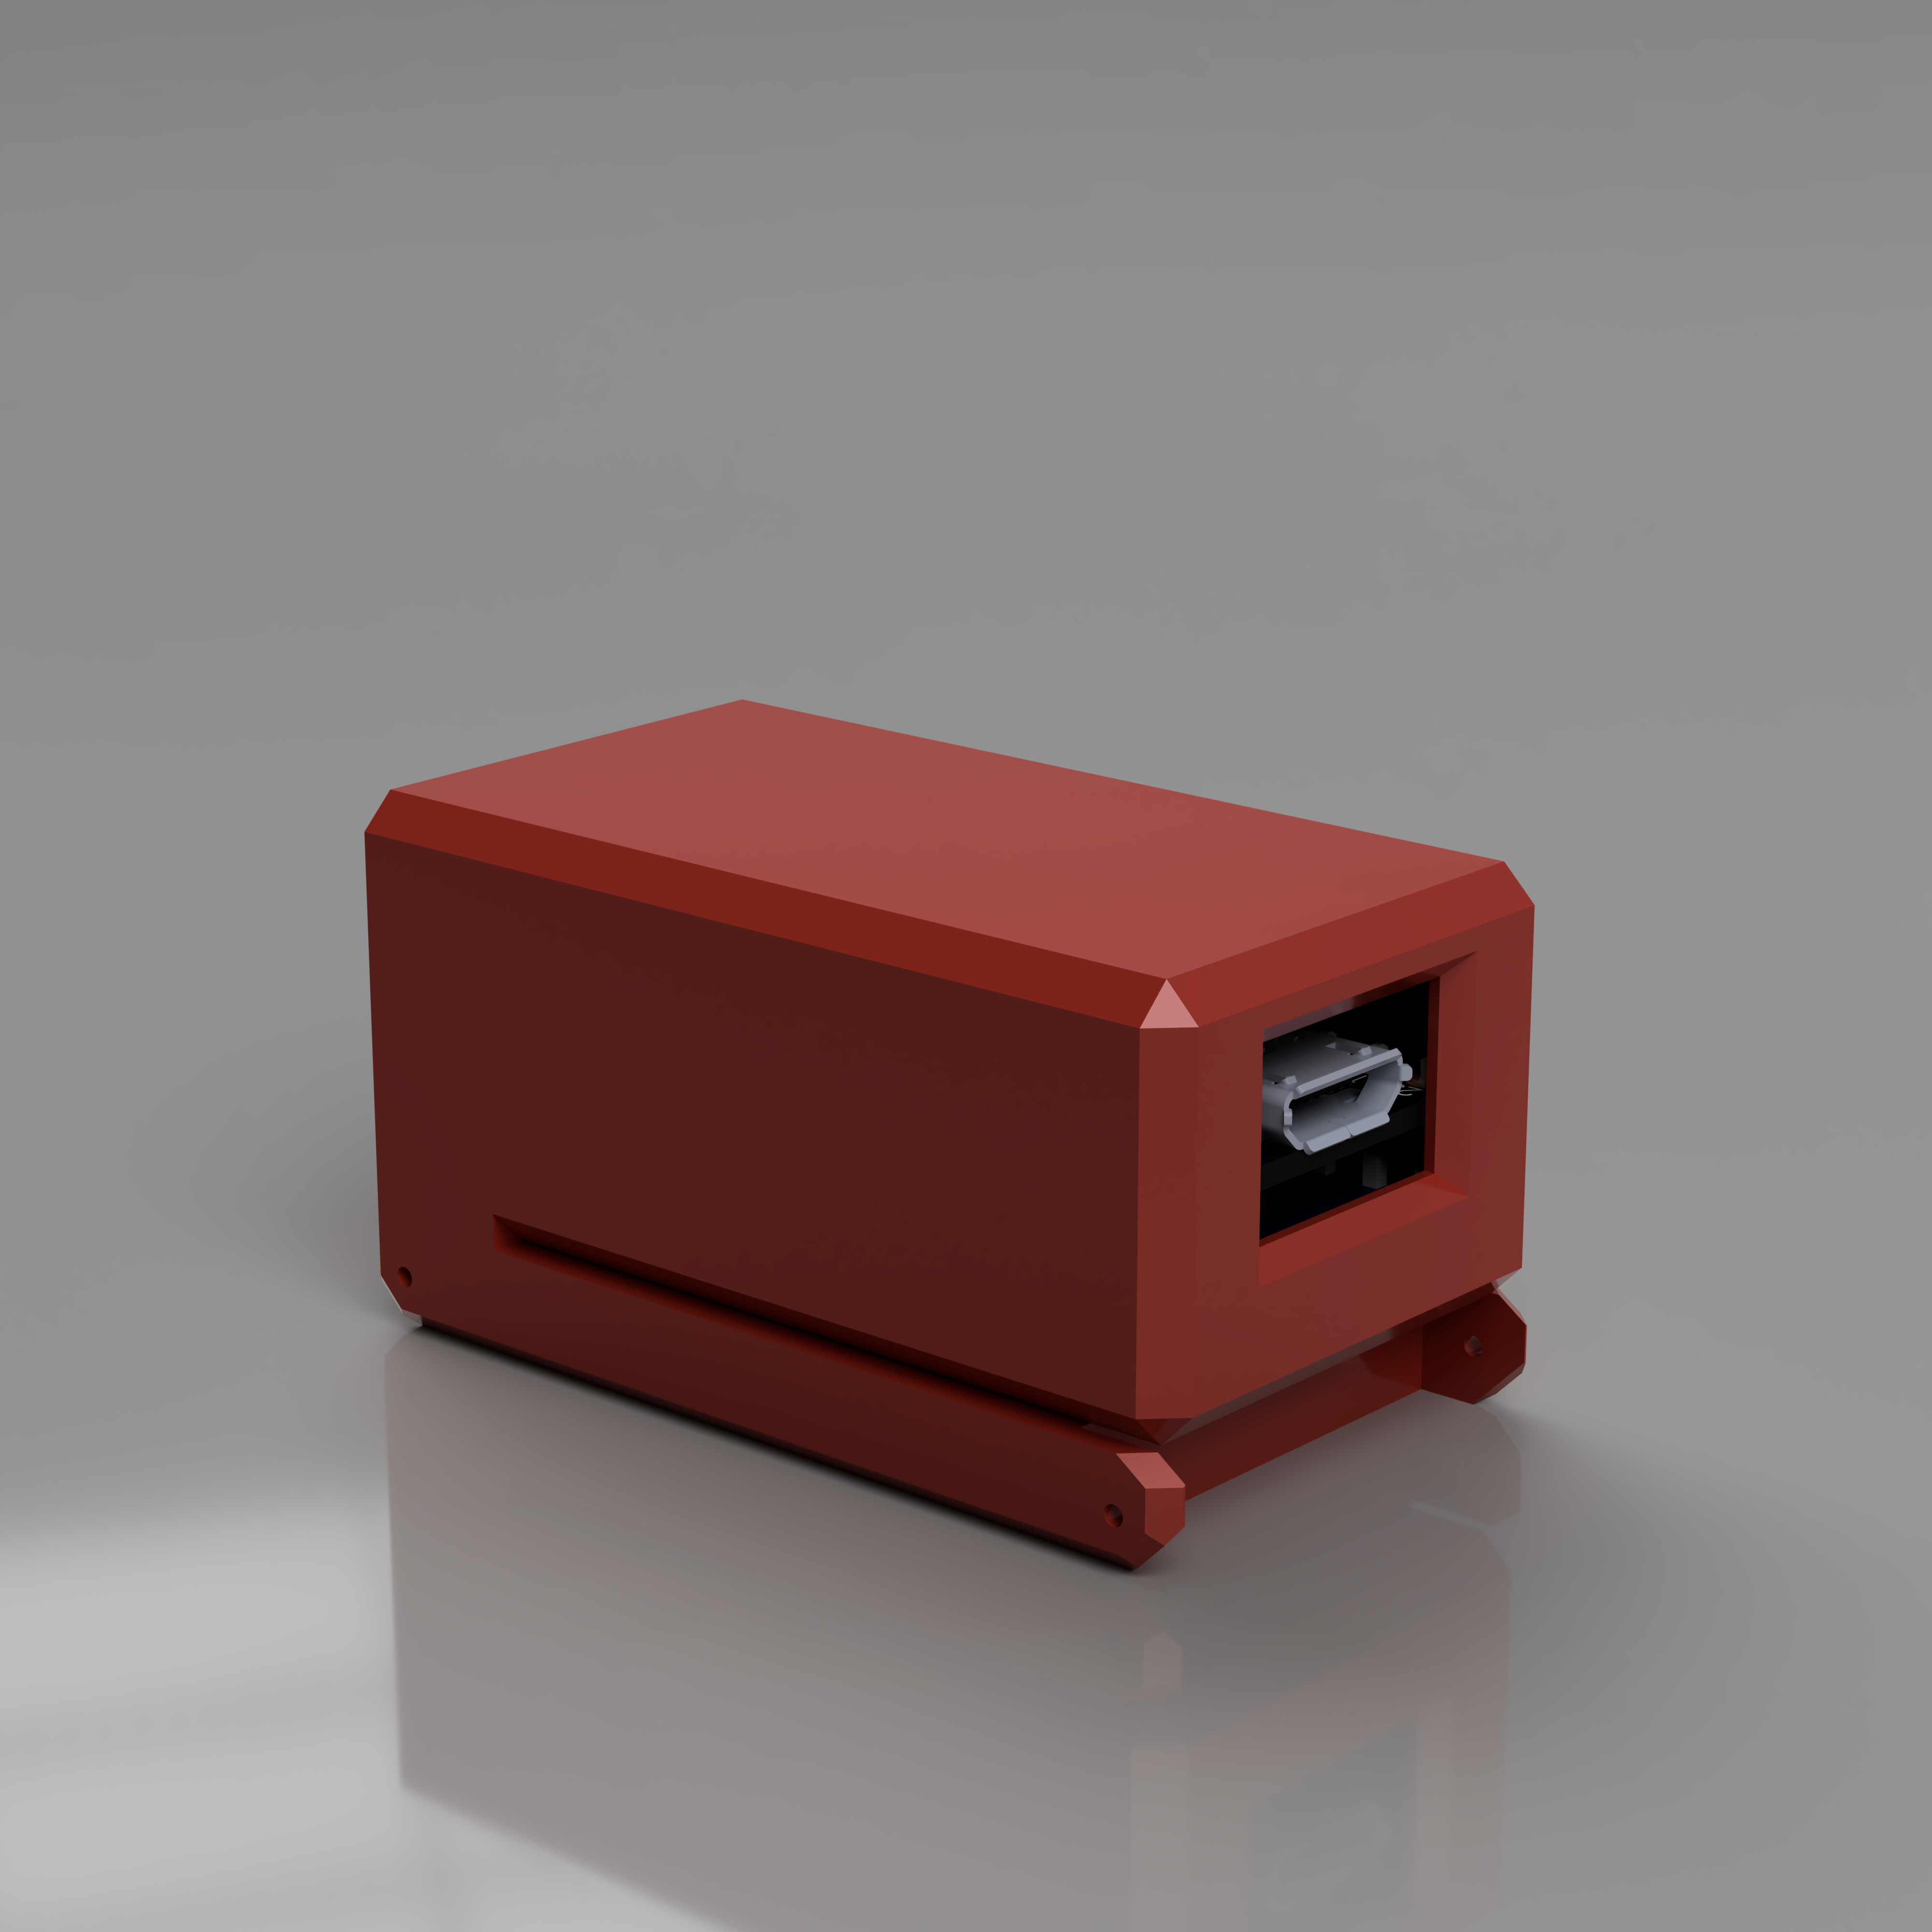
\includegraphics[width=.8\linewidth]{graphics/cad/wearable_strap_2.png}
  \captionsetup{width=0.8\linewidth, justification=centering}
  \centering
  \captionof{figure}{Wearable device with strap attachment}
  \label{fig:wearable_strap_2}
\end{minipage}
\end{figure}

        \subsection{Prototype}
        \label{subsec:Prototype_wearable}

        \subsection{UML}
        \label{sec:uml_wearable}
        
            This section will break down the software systems utilised in the walking aid device into formal language representations. These will take the form of a class diagram, which will illustrate the relationships between each of classes developed for the system, and an activity diagram which will demonstrate the sequence of events that will take place in the system and how they are handled. We hope that this section will help the reader to understand the software system in a broken down, step-by-step manner and to gain an understanding of our rationale towards programming choices that helped us to fulfil the user requirements. The class diagrams will be followed by an explanation of the role of each class and its functions, with the activity diagram also being accompanied by a body of text that establishes in natural language the sequence of events that will take place in the software system and how they are processed.

            \subsubsection{Class Diagram}
            \label{subsubsec:class_diagram_wearable}

                Similarly to the walking aid device section, this section will include the class and activity diagrams of the wearable device. Each diagram will be accompanied by a body of text that explains the diagram in a natural language format.

                \clearpage
                \thispagestyle{empty}
                \begin{landscape}
                    % [H] means put the figure HERE, directly when you input this code.
\begin{figure}[H]
	\centering
	\captionsetup{width=1.0\linewidth}

% We set the width of the figure based on the width of one line of text on the page.
% The value can be tuned to any value in [0.0, 1.0] to scale the image while maintaining its aspect ratio.

	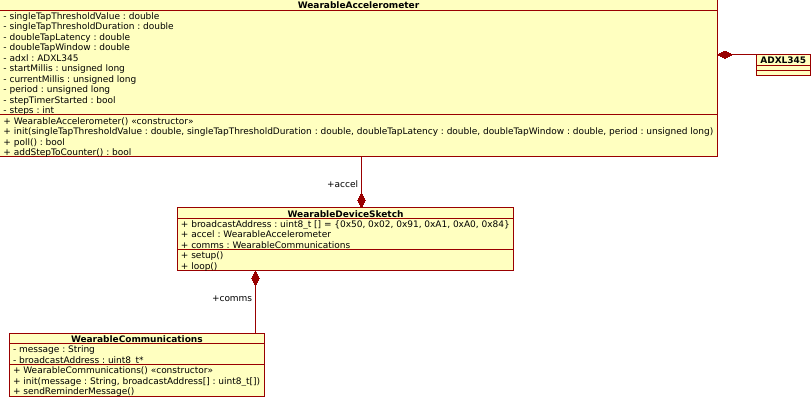
\includegraphics[width=1.0\linewidth]{./UML/WearableDevice/class diagram.png}

% Caption is defined with a short and long version. The short version is shown in the
% List of Figures section, and the long version is used directly with the figure.
	\caption[Wearable Device Class Diagram]{A class diagram for the wearable device software system illustrating how the classes interact with each other.}

% For figures label should be defined after the caption to ensure proper figure numbering.
	\label{fig:class_diagram_wearable}

\end{figure}
                \end{landscape}

                \paragraph{WearableDeviceSketch}\mbox{}

                    This is the main sketch for the wearable device system and implements the setup and loop functions necessary for an Arduino system. It creates instances of the WearableAccelerometer and WearableCommunications class to provide the full functionality of the wearable device. The setup function initialises both classes with the developer's selected parameters. Following this, the loop function handles the calls to check if the user has moved more than 5 steps within a period of time set by the developer. If they have, then the communications object is called to handle the broadcasting of a reminder message to the walking aid device.

                    The WearableDeviceSketch has a composition relationship to both of the other classes as it plays the role of instantiating both objects. Therefore, without the existence of the WearableDeviceSketch, an object of the other two classes would not exist.

                \paragraph{WearableCommunications}\mbox{}

                    The WearableCommunications class handles all the functionality needed to broadcast a message to the walking aid device. Once it is intialised by the WearableDeviceSketch class with a reminder message to send and a MAC address to send the message to, its sendReminderMessage function can be called to broadcast a reminder message when the user has walked more than 5 steps in a specified period of time set by the developer. It is also initialised with the details of the walking aid device as a peer to allow incmoming communication. The WearableCommunications class has a composition relationship with the DebugLED class to allow for the LED to be configured should an error occur with the initiation of the communication protocol.

                    This class is also part of a composition relationship with the WearableDeviceSketch class and therefore an object of it cannot exist unless the WearableDeviceSketch class is instantiated.

                \paragraph{DebugLED}\mbox{}

                    The DebugLED class exists to handle the configuration of the TinyPICO's onboard LED to indicate whether the communication protocol is working or not. It is initialised in the WearableDeviceSketch class and is therefore part of a composition relationship with the WearableCommunications class. More specifically, an instance of the DebugLED class cannot exist without an instance of the WearableCommunications class.

                    The DebugLED class also holds a composition relationship with the TinyPICO helper library to allow for the configuration of the LED.

                \paragraph{WearableAccelerometer}\mbox{}

                    Controlling the functionality of the walking detection, this class utilises the ADXL345 accelerometer library to detect single-taps or gravitational changes through the accelerometer. Once it is initialised with threshold values and a value for the period of time used to check for 5 steps, the poll function can be called by the WearableDeviceSketch to check for steps. Each time a step is detected, the addStepToCounter function is called to add to the total number of steps detected. If a step is detected, and it has taken more than the period of time since the first step is detected, then the timer is reset. Otherwise, if the step counter is incremented and is still less than 5 steps, then we move on. However, if the step counter reaches 5 steps within the developer set period of time, then a true boolean value is returned to the WearableDeviceSketch to notify it that a reminder message should be sent to the walking aid device.

                    The class holds a composition relationship with the ADXL345 library to retrieve the necessary functionality for step detection. This class is also part of a composition relationship with the WearableDeviceSketch class, meaning that if an instance of the WearableDeviceSketch class does not exist then neither will an instance of this class. 

                \newpage

            \subsubsection{Activity Diagram}
            \label{subsubsec:wearable_activity}

                The following is an activity diagram that demonstrates the workflow of the wearable software system. The diagram demonstrates how the system attempts to detect that the user is walking in a step-by-step manner to provide clarity of how the software was developed for these purposes. Accompanying the diagram will be a body of text that describes the process in natural language.

                % [H] means put the figure HERE, directly when you input this code.
\begin{figure}[H]
	\centering
	\captionsetup{width=1.0\linewidth}

% We set the width of the figure based on the width of one line of text on the page.
% The value can be tuned to any value in [0.0, 1.0] to scale the image while maintaining its aspect ratio.

	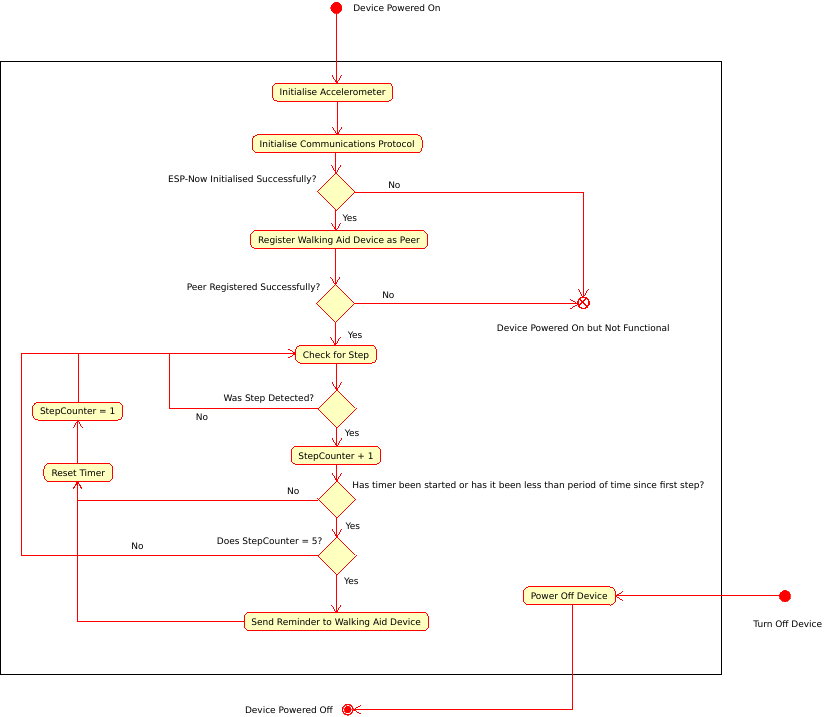
\includegraphics[width=1.0\linewidth]{./UML/WearableDevice/activity diagram.png}

% Caption is defined with a short and long version. The short version is shown in the
% List of Figures section, and the long version is used directly with the figure.
	\caption[Wearable Device Activity Diagram]{An activity diagram for the wearable device software system illustrating the workflow of the system.}

% For figures label should be defined after the caption to ensure proper figure numbering.
	\label{fig:activity_diagram_wearable}

\end{figure}

                The activity diagram demonstrates that the system begins when the device is powered on. The system begins by initialising the accelerometer with the configurations of the developer before attempting to initialise the ESP-Now communications protocol and registering the walking aid device as a peer for communication. If either of ESP-Now steps fail then we end up in a state where the device is powered on but is not functional. 

                If the communication initialisation is successful, then we begin the process of attempting to identify when the user is walking. We begin first by checking for a step, which in actual fact checks if the accelerometer has detected a change in gravity. If it has not detected a step, then we loop back and check for a step again until we identify one. Otherwise, we increment the step counter before checking to see if the timer has started and if it has, then we check to see if the time since the first step was detected is greater than the period of time set by the developer. If the timer has not been started, or it has been greater than the developer specified period of time since the first step, we reset the timer and set the step counter back to 1 and start the check for step process again. Otherwise, we run a check to see if the step counter is now at 5 steps. If it is not, then we loop back to the beginning of the check for step counter. If the step counter is indeed equal to 5, then we have reached the situation where the user has moved a considerable amount in the period of time set by the developer. We can therefore ascertain that the user is walking and send a reminder message to the walking aid device to check if the walking aid is moving as well.

                Finally, despite it not following activity diagram etiquette, we wanted to demonstrate how powering off the system is the only way to stop the device from being functional. The existence of a second initial activity that controls the powering off of the system demonstrates this, and demonstrates how the rest of the system relies on the device being powered on.

    \section{Common designs between the Walking Aid and the Wearable Devices}
    \label{sec:both_devices}

        This section will contain information on the design decisions we made that impacted both the wearable and walking aid devices. This will include software and hardware decisions that allowed us to implement a communications system, that allowed us to keep device form factor and power usage to a minimum, and discussion of why we chose pieces of hardware that are common between both devices.

        \subsection{Development Board - TinyPICO}
        \label{subsec:development_board}

            The development board for each device would provide the necessary communication between multiple hardware components to allow us to reach the originally defined user requirements. Due to our previous experience with ESP32 chips and due to the necessity of our devices being of a small enough form factor to fit on the limbs of patients and on walking aids, we decided to use the TinyPICO development boards. Their use of ESP32 chips provide the basis for our communication system which utilises a Wi-Fi module, and provides adequate pin outs to allow us to communicate to each hardware device that we include within our systems. This is all achieved whilst keeping power usage to a minimum and allowing us to meet the client requirement of creating devices that are able to operate for a substantial amount of time without the need for battery replacements. The 240MHz dual-core chip that is the ESP32, would provide performance that allows our system to react to incoming communication from the Wi-Fi module or accelerometer promptly to provide a responsive system for our clients. The vast documentation supporting the development of embedded systems using ESP32s was instrumental in the success of our project, and we feel that the decision to utilise TinyPICO development boards was the correct one because of it. We were also influenced to use TinyPICO development boards due to Swansea University allowing us to borrow two boards at no extra cost, which ultimately allowed us to remain within our £150 budget. Finally, the TinyPICO boards also provide a built-in LED which we utilised throughout project development for debugging purposes.

        \subsection{Programming Language - Arduino C (C/C++)}
        \label{subsec:programming_language}

            We decided to utilise the Arduino C (C++) programming language rather than using MicroPython to develop our embedded software due to C++'s superior efficiency over Python for the development of embedded software \cite{github_2014, dicola}. Other tools such as PlatformIO would have provided the basis to allow us to utilise C++ for our software development, but due to the benefits of our team having previous experience of using the Arduino IDE to develop embedded systems, espetially in the field of software development with ESP32 chips, we felt that our project would be better suited to being developed utilising the Arduino ecosystem. We were also aware that the handover of this project would mean that another team would be able to take on the role of advancing our code and felt that C++ provided the best platform for developing smaller and more self-explanatory code across multiple header and implementation files. This would mean that any developers that attempt to further develop our code in future, should find it rather simple to identify what each class and block of code is attempting to accomplish.

        \subsection{Accelerometer - Adafruit ADXL345}
        \label{subsec:accel}

            Within this project, the accelerometer would provide the basis for identifying movement of the patient and the walking aid. The vast documentation supporting the development of embedded systems using ADXL345 accelerometers was a substantial factor in why we opted to include them in our systems. They provide the functionality for the detection of various changes in acceleration such as activity detection, free fall detection and single-tap and double-tap detection. The single-tap detection feature of the ADXL345 provides the basis for movement detection on both devices due to the fact that it can detect changes in gravity to identify when a step has been taken. The single-tap detection feature also allows the system to still be utilised whether the user is wearing the wearable device on their wrist or ankle, with the single-tap detection feature also being able to detect when the walking aid is being lifted and placed back on the ground. The free fall detection feature provided by the ADXL means that future developers will be able to easily implement a free fall detection system, which would allow the client to have their stretch goal implemented into the project. We opted to use the ADXL345 over other accelerometers as it is one of the newer offerings of accelerometers from the well renowned and reliable brand, Adafruit. Because of this, the accelerometers were relatively easy and quick to source, whilst only costing £7 per unit and allowing us to remain within our £150 budget. Finally, with the walking aid's TinyPICO already having its Serial Peripheral Interface and 3.3V power pin outs being utilised by the I2S audio shield, the ADXL345 allowed us to use the TinyPICO's I\textsuperscript{2}C interface for communication between the accelerometer and the development board, and allowed us to use the 5V pin out provided by the TinyPICO to power the ADXL345 due to its built-in voltage regulator.

        \subsection{Communication Protocol - ESP-Now}
        \label{subsec:esp_now_comms}

            Within the details specified in our Milestone 2 interim progress report, we classified the advantages and disadvantages of various options for communication protocols for use within our project. The first of those communication protocols was ESP-Now, a communication technology developed by the creators of the ESP32 chip, Espressif, which utilises the ESP32's Wi-Fi module to communicate with other devices that contain ESP32 chips \cite{esp-now_overview}. The other two communication protocol options we could have utilised were Bluetooth Low Energy (BLE) and Ultra-wideband (UWB). Despite considerations to include the use of UWB within our project, it would have been far too expensive for us to implement, and thus we instantly rejected the notion of using UWB within our project. Therefore, we were left with a decision to either utilise BLE or ESP-Now for the communication standard between our walking aid and wearable device. For the rest of this section, we will detail the advantages and disadvantages to using ESP-Now for our communication system, with comparisons to BLE, before finally detailing why we ultimately opted to utilise ESP-Now.

            \newpage
            \subsubsection{Advantages and Disadvantages of ESP-Now with comparisons to BLE}
            \label{subsubsec:esp_now_advantages_disadvantages}

                \vspace{2em}
                \small
		\begin{xltabular}[H]{\textwidth}{p{0.47\textwidth} | p{0.47\textwidth}}
			\caption[ESP-Now Advantages and Disadvantages]{A table listing the advantages and disadvantages of the ESP-Now protocol.}\\

			\toprule

		 	Advantages & Disadvantages\\

			\midrule
			\endfirsthead

			\toprule

			Advantages & Disadvantages\\

			\midrule
			\endhead

			\hline
			\multicolumn{2}{|r|}{{Continued on next page}}\\
			\hline
			\endfoot

			\bottomrule
			\endlastfoot

			Provides a simple implementation of two-way communication between ESP32s \cite{random_nerd_tutorials}. This would allow us to easily send messages between the wearable and walking aid device to check if either are moving.
			
			&
			
			Similar to UWB, it is only adoptable for ESP chips and therefore less adopted in this area than BLE, meaning we will be limited to using ESP chipped boards for future product development, or we would have to redevelop our communication system.\\
			
			\midrule
			
			Maximum message sizes are limited to 250 bytes \cite{random_nerd_tutorials}. Similar to the advantage stated with BLE, a small message size means minimal overheads, which is beneficial to our project as we will only be sending short signal messages between devices.
			
			&
			
			ESP-Now is less power efficient than BLE \cite{neupane_2019} and in turn less power efficient than UWB \cite{bender_2021}. This would mean that the patient or carer would need to remember to change the batteries in our devices more often.\\
			
			\midrule
			
			The ESP-Now library includes callbacks \cite{random_nerd_tutorials} that can allow our devices to notice whether their messages to the other devices have been received successfully or not. This can create a more robust communication protocol that attempts to avoid lost packets. This will mean that reminders that should be played to the patient are less likely to fail.
			
			&
			
			\\
			
			\midrule
			
			ESP-Now was developed for the ESP32 chips found on our TinyPICO boards. Because of this, the documentation provided that directly relates to our hardware is perfect for code development and lessens the difficulty of developing our communication protocol.
			
			&
			
			\\

		\end{xltabular} 
		\label{tbl:now}
                \vspace{5em}

                We ultimately decided to use ESP-Now as our communication protocol due to its ease of implementation and due to the fact that it allows sketch sizes to be smaller \cite{random_nerd_tutorials} than the sketch sizes of BLE \cite{kolban_2018}. The significance to sketch sizes being smaller is that they allow for the larger memory storage spaces accounting for larger audio reminder files, as well as providing more responsive code for what is a time sensitive system. The lower throughput that ESP-Now provides in comparison to BLE should not be noticeable within our system due to the fact that we only ever send one word messages between our devices at a given time. However, the lower power efficiency of ESP-Now in comparison to BLE is a considerable disadvantage for use within this system. Having said this, ESP-Now is still regarded as being a low power solution and should still mean that the patient or carer will not need to remember to replace the batteries in their devices too often.


        \subsection{Power}
        \label{subsec: Power}
            Our prototypes will not include any battery or portable power source support built in, this decision was made due to the limited time and budget we had. Our vision, research and hardware supports 1S Lithium Polymer (LiPo) batteries as standard, and the TinyPico is designed to be used with this power source in mind. Unfortunately, researching safe battery charging circuits as well as proper battery care was not something we had the time for, and will leave as an attainable stretch goal if this project were to gain further funding or time budgets.

            \todo{Add pictures of 1s lipos}

            1S LiPos are compact, and offer excellent discharge currents which would make it ideal for our high wattage speaker, although adjusting speaker size can reduce the battery requirement quite significantly, and can be considered later on with further research and testing.

            Our prototypes are powered by the same MicroUSB, 5V port that is used for programming and updating the device, to facilitate testing, these will run off of portable power banks with USB outputs, to ensure reliable voltage and amperage is provided to our devices to reduce potential issues during testing.

        \subsection{Prototyping}
        \label{subsec: Prototyping}
        
            \todo{Add software citations}
            The software package used for designing the prototypes was chosen to be Autodesk Fusion 36, as well as how pervasive it is within the 3D Printing community.

            Where possible, we ensured to use accurate existing models. This allowed us to make progress faster, as working out and modelling tight tolerances on PCB components wasn't always required. 

            For the hardware we could not find models for, such as the speaker, i2s audio shield, and vibration motor, critical dimensions were taking using Vernier calipers, and by cross checking datasheets for each or similar devices.

            For both devices, a large emphasis was placed on creating an enclosure for the electronics with a minimal, but modular form factor. As shown in their respective sections, the devices were designed to effectively house and protect the existing components, as well as allow for future expansion using modular systems and design choices, such as extendable mid plates and standard sized screws and fasteners.

            Once designs for the enclosures were created, they were sliced and converted to gcode using the open source software package SuperSlicer, and then printed on a custom VoronDesign 0.1 CoreXY Fused Filament Deposition (FDM) 3D Printer. SuperSlicer was chosen due to our teams experience with the software, as well as already having a previously tuned profile for the machine.

            The material for printing was chosen to be Acrylonitrile butadiene styrene (ABS), a ubiquitous thermoplastic most often used with injection moulding in everyday objects due to its high impact resistance and thermal/checmical resistance. It used to be the plastic of choice for hobby grade 3D Printing, however is becoming less common vs easier to print, and weaker/biodegradable plastics like Polylactic Acid (PLA) or Polyethylene terephthalate (PETG). We chose to continue with ABS, as our printer is cable of printing this more exotic material, and its properties will us to undertaken stricter impact and resistance testing.             
        
    \newpage

    \section{Class Documentation - Walking Aid Device}
    \label{sec:class_documentation_walk_aid}\mbox{}

        \subsection{SDToSPIFFS Class Reference}
        \label{subsec:sdtospiffs}\mbox{}

                \paragraph{Public Member Functions}\mbox{}

                    \begin{itemize}
                        \item \textbf{SDToSPIFFS}() 
                        
                            \textit{Construct a new SDToSPIFFS object.}

                        \item void \textbf{init}(const char *SDPath, const char* SPIFFSPath) 
                        
                            \textit{Initalises the object ready for the transferring of files from SD card to SPIFFS.}

                        \item \textbf{loadSDFileToSPIFFS}() 
                        
                            \textit{Handles the loading of the SD card file to SPIFFS.}

                        \item const char *\textbf{getSPIFFSPath}() 
                        
                            \textit{Returns the path to the SPIFFS file.}
                    \end{itemize}

            \subsubsection{Member Function Documentation}\mbox{}

                \paragraph{SDToSPIFFS()}\mbox{}\\

                    \ttfamily{SDToSPIFFS::SDToSPIFFS (  )}\\

                    \rmfamily{Construct a new SDToSPIFFS object.}

                \paragraph{init()}\mbox{}\\

                    \ttfamily{void SDToSPIFFS::init (\\
                        \null \quad \quad \quad \quad \quad \quad \quad \quad \quad const char * SDPath,\\ 
                        \null \quad \quad \quad \quad \quad \quad \quad \quad \quad const char * SPIFFSPath )}\\

                    \rmfamily{Returns the path to the SPIFFS file.}

                    \textbf{Parameters}

                    \vspace{1em}
                    \begin{tabular}{| l | l |} 
                        \hline
                        SDPath & The path to the SD card file. \\ 
                        \hline
                        SPIFFSPath & The file name to give the new SPIFFS file. \\ 
                        \hline
                    \end{tabular}

                \paragraph{loadSDFileToSPIFFS()}\mbox{}\\

                    \ttfamily{void SDToSPIFFS::loadSDFileToSPIFFS (  )}\\
    
                    \rmfamily{Handles the loading of the SD card file to SPIFFS.}

                \paragraph{getSPIFFSPath()}\mbox{}\\

                    \ttfamily{const char * SDToSPIFFS::getSPIFFSPath (  )}\\

                    \rmfamily{Returns the path to the SPIFFS file.}

                    \textbf{Returns}

                        \quad \quad const char* SPIFFS file path.
        \newpage
        \subsection{WalkAidAccelerometer Class Reference}
\label{subsec:WalkAidAccelerometer}\mbox{}

    \ttfamily{}

    \#include <WalkAidAccelerometer.h>\\

    \rmfamily{}

    \paragraph{Private Attributes}\mbox{}\\

        \begin{itemize}
            \item double \textbf{singleTapThresholdValue}
            
                \quad \quad \textit{Threshold for single tap to be detected.}

            \item double \textbf{singleTapThresholdDuration}
            
                \quad \quad \textit{Duration for single tap to be above threshold to be detected.}

            \item double \textbf{doubleTapLatency}
            
                \quad \quad \textit{Time between a tap event and when the reading for a double tap starts.}

            \item double \textbf{doubleTapWindow}
            
                \quad \quad \textit{Defines how long a double tap is checked for.}

            \item bool \textbf{stepDetected}
            
                \quad \quad \textit{Defines if a step has been detected.}

            \item long \textbf{lastStepTime}
            
                \quad \quad \textit{The last time a step was detected.}

            \item unsigned long \textbf{period}
            
                \quad \quad \textit{The period to check previously and in future for detected steps.}

            \item ADXL345 \textbf{adxl}
            
                \quad \quad \textit{Accelerometer object.}\\

        \end{itemize}


    \paragraph{Public Member Functions}\mbox{}\\

        \begin{itemize}
            \item \textbf{WalkAidAccelerometer}() 
            
                \quad \quad \textit{Construct a new Walk Aid Accelerometer object.}

            \item void \textbf{init}(double singleTapThresholdValue, double singleTapThresholdDuration
            , \\double doubleTapLatency, double doubleTapWindow, unsigned long period) 
            
                \quad \quad \textit{Initialises the accelerometer with the specified values in parameter fields.}

            \item bool \textbf{checkForStep}() 
            
                \quad \quad \textit{Checks if a tap event was detected by the accelerometer.}

            \item bool \textbf{isStepDetected}() 
            
                \quad \quad \textit{Returns the value of stepDetected.}

            \item long \textbf{getLastStepTime}() 
            
                \quad \quad \textit{Get the time the last step was taken.}

            \item unsigned long \textbf{getPeriod}() 
            
                \quad \quad \textit{Get the developer's specified period to check for steps.}\\

        \end{itemize}

    \subsubsection{Constructor \& Destructor Documentation}\mbox{}


        \paragraph{WalkAidAccelerometer()}\mbox{}\\

            \ttfamily{WalkAidAccelerometer::WalkAidAccelerometer (  )}\\

            \rmfamily{Construct a new Walk Aid Accelerometer object.}\\


    \subsubsection{Member Function Documentation}\mbox{}


        \paragraph{init()}\mbox{}\\

            \ttfamily{void WalkAidAccelerometer::init (\\
                \null \quad \quad \quad \quad \quad \quad \quad \quad \quad double singleTapThresholdValue,\\ 
                \null \quad \quad \quad \quad \quad \quad \quad \quad \quad double singleTapThresholdDuration,\\ 
                \null \quad \quad \quad \quad \quad \quad \quad \quad \quad double doubleTapLatency,\\
                \null \quad \quad \quad \quad \quad \quad \quad \quad \quad double doubleTapWindow,\\
                \null \quad \quad \quad \quad \quad \quad \quad \quad \quad unsigned long period)}\\

            \rmfamily{Initialises the accelerometer with the specified values in parameter fields.}

            \textbf{Parameters}

            \vspace{1em}
            \begin{tabular}{| l | l |} 
                \hline
                singleTapThresholdValue & Threshold for single tap to be detected.\\ 
                \hline
                singleTapThresholdDuration & Duration that tap must be above threshold to be detected.\\ 
                \hline
                doubleTapLatency & Time after single tap until double tap is measured.\\ 
                \hline
                doubleTapWindow & How long double tap is checked for.\\ 
                \hline
                period & Time period to check for steps before and after receiving message.\\ 
                \hline
            \end{tabular}\\~\\


        \paragraph{checkForStep()}\mbox{}\\

            \ttfamily{bool WalkAidAccelerometer::checkForStep (  )}\\

            \rmfamily{Checks if a tap event was detected by the accelerometer.}\\

            \textbf{Returns}

                \quad \quad true if tap is detected, false otherwise.\\


        \paragraph{isStepDetected()}\mbox{}\\

            \ttfamily{bool WalkAidAccelerometer::isStepDetected (  )}\\

            \rmfamily{Returns the value of stepDetected.}

            \textbf{Returns}

                \quad \quad bool stepDetected\\

        \paragraph{getLastStepTime()}\mbox{}\\

            \ttfamily{long WalkAidAccelerometer::getLastStepTime (  )}\\

            \rmfamily{Get the time the last step was taken.}

            \textbf{Returns}

                \quad \quad long lastStepTime.\\

        \paragraph{getPeriod()}\mbox{}\\

            \ttfamily{unsigned long WalkAidAccelerometer::getPeriod (  )}\\

            \rmfamily{Get the developer's specified period to check for steps.}

            \textbf{Returns}

                \quad \quad unsigned long period.\\
        \newpage
        \subsection{WalkAidAudio Class Reference}
\label{subsec:WalkAidAudio}\mbox{}

    \ttfamily{}

    \#include <WalkAidAudio.h>\\

    \rmfamily{}

    \paragraph{Private Attributes}\mbox{}\\

        \begin{itemize}
            \item AudioGeneratorMP3 * \textbf{mp3}
            
                \quad \quad \textit{The generator of the mp3 player.}

            \item AudioFileSourceSPIFFS * \textbf{file}
            
                \quad \quad \textit{The source file of the SPIFFS audio file.}

            \item AudioOutputI2S * \textbf{out}
            
                \quad \quad \textit{The output of the mp3 player.}

            \item AudioFileSourceID3 * \textbf{id3}
            
                \quad \quad \textit{Metadata handler for the mp3 file.}

            \item SDToSPIFFS \textbf{s2s}
            
                \quad \quad \textit{Object to handle the SD to SPIFFS transfer.}\\

        \end{itemize}


    \paragraph{Public Member Functions}\mbox{}\\

        \begin{itemize}
            \item \textbf{WalkAidAudio}() 
            
                \quad \quad \textit{Construct a new Walk Aid Audio object.}

            \item void \textbf{init}(const char *SDPath, const char *SPIFFSPath) 
            
                \quad \quad \textit{Initialises the accelerometer with the specified values in parameter fields.}

            \item void \textbf{play}() 
            
                \quad \quad \textit{Plays the SPIFFS audio file.}\\

        \end{itemize}

    \subsubsection{Constructor \& Destructor Documentation}\mbox{}


        \paragraph{WalkAidAudio()}\mbox{}\\

            \ttfamily{WalkAidAudio::WalkAidAudio (  )}\\

            \rmfamily{Construct a new Walk Aid Audio object.}\\


    \subsubsection{Member Function Documentation}\mbox{}


        \paragraph{init()}\mbox{}\\

            \ttfamily{void WalkAidAudio::init (\\
                \null \quad \quad \quad \quad \quad \quad \quad \quad \quad const char * SDPath,\\ 
                \null \quad \quad \quad \quad \quad \quad \quad \quad \quad const char * SPIFFSPath)}\\

            \rmfamily{Initialises the walk aid audio system by calling the transfer of SD file to SPIFFS and generating the}

            mp3 code.

            \textbf{Parameters}

            \vspace{1em}
            \begin{tabular}{| l | l |} 
                \hline
                SDPath & Path to the SD card audio file.\\ 
                \hline
                SPIFFSPath & Name of the SPIFFS audio file to be created.\\ 
                \hline
            \end{tabular}\\~\\


        \paragraph{play()}\mbox{}\\

            \ttfamily{void WalkAidAudio::play (  )}\\

            \rmfamily{Plays the SPIFFS audio file.}\\
        \newpage
        \subsection{WalkAidCommunications Class Reference}
\label{subsec:WalkAidCommunications}\mbox{}

    \ttfamily{}

    \#include <WalkAidCommunications.h>\\

    \rmfamily{}

    \paragraph{Private Attributes}\mbox{}\\

        \begin{itemize}
            \item bool \textbf{reminder}
            
                \quad \quad \textit{Whether a reminder message has been received.}\\

        \end{itemize}


    \paragraph{Public Member Functions}\mbox{}\\

        \begin{itemize}
            \item \textbf{WalkAidCommunications}() 
            
                \quad \quad \textit{Construct a new Walk Aid Communications object.}

            \item void \textbf{init}()
            
                \quad \quad \textit{Initialise communication to the wearable device.}

            \item bool \textbf{getReminder}() 
            
                \quad \quad \textit{Get whether a reminder has been received or not.}
                
            \item void \textbf{setReminder}(bool reminder) 
            
                \quad \quad \textit{Set whether a reminder has been received or not.}\\

        \end{itemize}

    \subsubsection{Constructor \& Destructor Documentation}\mbox{}


        \paragraph{WalkAidCommunications()}\mbox{}\\

            \ttfamily{WalkAidCommunications::WalkAidCommunications (  )}\\

            \rmfamily{Construct a new Walk Aid Communications object.}\\


    \subsubsection{Member Function Documentation}\mbox{}


        \paragraph{init()}\mbox{}\\

            \ttfamily{void WalkAidCommunications::init ()}\\

            \rmfamily{Initialise communication to the wearable device.}

        \paragraph{getReminder()}\mbox{}\\

            \ttfamily{bool WalkAidCommunications::getReminder (  )}\\

            \rmfamily{Get whether a reminder has been received or not.}

            \textbf{Returns}

                \quad \quad bool reminder.\\


        \paragraph{setReminder()}\mbox{}\\

            \ttfamily{void WalkAidCommunications::setReminder (  )}\\

            \rmfamily{Set whether a reminder has been received or not.}

            \textbf{Parameters}

            \vspace{1em}
            \begin{tabular}{| l | l |} 
                \hline
                reminder & true if reminder received, false otherwise.\\ 
                \hline
            \end{tabular}\\~\\
        \newpage
        \subsection{DebugLED Class Reference}
\label{subsec:debugled2}\mbox{}

    \ttfamily{}

    \#include <DebugLED.h>\\

    \rmfamily{}

    \paragraph{Private Attributes}\mbox{}\\

        \begin{itemize}
            \item TinyPICO \textbf{tp}
            
                \quad \quad \textit{The TinyPICO object used to control the LEDs.}\\

        \end{itemize}


    \paragraph{Public Member Functions}\mbox{}\\

        \begin{itemize}
            \item \textbf{DebugLED}() 
            
                \quad \quad \textit{Construct a new DebugLED object.}

            \item void \textbf{poweredOn}() 
            
                \quad \quad \textit{Displays a green LED for 1 second to signify successful power on.}

            \item void \textbf{initError}() 
            
                \quad \quad \textit{Displays a red LED to signify ESP-Now init error.}

            \item void \textbf{peerSetupError}() 
            
                \quad \quad \textit{Displays an orange LED to signify an ESP-Now peer connection error.}\\
        \end{itemize}

    \subsubsection{Constructor \& Destructor Documentation}\mbox{}


        \paragraph{DebugLED()}\mbox{}\\

            \ttfamily{DebugLED::DebugLED (  )}\\

            \rmfamily{Construct a new DebugLED object.}\\


    \subsubsection{Member Function Documentation}\mbox{}


        \paragraph{poweredOn()}\mbox{}\\

            \ttfamily{void DebugLED::poweredOn (  )}\\

            \rmfamily{Displays a green LED for 1 second to signify successful power on.}\\


        \paragraph{initError()}\mbox{}\\

            \ttfamily{void DebugLED::initError (  )}\\

            \rmfamily{Displays a red LED to signify ESP-Now init error.}\\


        \paragraph{peerSetupError()}\mbox{}\\

            \ttfamily{void DebugLED::peerSetupError (  )}\\

            \rmfamily{Displays an orange LED to signify an ESP-Now peer connection error.}\\
        \newpage
        \subsection{Sketch Class Reference}
\label{subsec:sketch}\mbox{}

    \paragraph{Public Attributes}\mbox{}\\

        \begin{itemize}
            \item String \textbf{message}
            
                \quad \quad \textit{A copy of the message received from the wearable device.}

            \item WalkAidAudio \textbf{audio}
            
                \quad \quad \textit{The audio controller object.}

            \item WalkAidCommunications \textbf{comms}
            
                \quad \quad \textit{The communications controller object.}
                
            \item WalkAidAccelerometer \textbf{accel}
            
                \quad \quad \textit{The accelerometer controller object.}\\

        \end{itemize}


    \paragraph{Public Member Functions}\mbox{}\\

        \begin{itemize}
            \item void \textbf{setup}() 
            
                \quad \quad \textit{Handles the Arduino setup function. Initialises the accelerometer, communications, and audio.}

            \item void \textbf{loop}() 
            
                \quad \quad \textit{Handles the Arduino loop function. Loops through checks for reminder messages and responds accordingly.}\\
        \end{itemize}


    \subsubsection{Member Function Documentation}\mbox{}


        \paragraph{setup()}\mbox{}\\

            \ttfamily{void setup (  )}\\

            \rmfamily{Handles the Arduino setup function. Initialises the accelerometer, communications, and audio.}


        \paragraph{loop()}\mbox{}\\

            \ttfamily{void loop (  )}\\

            \rmfamily{Handles the Arduino loop function. Loops through checks for reminder messages and responds accordingly.}\\
        \newpage

    \section{Class Documentation - Wearable Device}
    \label{sec:class_documentation_wearable}\mbox{}

        \subsection{WearableAccelerometer Class Reference}
\label{subsec:WearableAccelerometer}\mbox{}

    \ttfamily{}

    \#include <WearableAccelerometer.h>\\

    \rmfamily{}

    \paragraph{Private Attributes}\mbox{}\\

        \begin{itemize}
            \item double \textbf{singleTapThresholdValue}
            
                \quad \quad \textit{Threshold for single tap to be detected.}

            \item double \textbf{singleTapThresholdDuration}
            
                \quad \quad \textit{Duration for single tap to be above threshold to be detected.}

            \item double \textbf{doubleTapLatency}
            
                \quad \quad \textit{Time between a tap event and when the reading for a double tap starts.}

            \item double \textbf{doubleTapWindow}
            
                \quad \quad \textit{Defines how long a double tap is checked for.}

            \item ADXL345 \textbf{adxl}
            
                \quad \quad \textit{Accelerometer object.}

            \item unsigned long \textbf{startMillis}
            
                \quad \quad \textit{Keeps track of when the first step was taken.}

            \item unsigned long \textbf{currentMillis}
            
                \quad \quad \textit{Stores the time of the current step being taken.}

            \item unsigned long \textbf{period}
            
                \quad \quad \textit{The period to check previously and in future for detected steps.}
                
            \item bool \textbf{stepTimerStarted}
            
                \quad \quad \textit{Stores if the timer has been started or not.}
                
            \item int \textbf{steps}
            
                \quad \quad \textit{Acts as the step counter.}\\

        \end{itemize}


    \paragraph{Public Member Functions}\mbox{}\\

        \begin{itemize}
            \item \textbf{WearableAccelerometer}() 
            
                \quad \quad \textit{Construct a new Wearable Accelerometer object.}

            \item void \textbf{init}(double singleTapThresholdValue, double singleTapThresholdDuration
            , \\double doubleTapLatency, double doubleTapWindow, unsigned long period) 
            
                \quad \quad \textit{Initialises the accelerometer with the specified values in parameter fields.}

            \item bool \textbf{poll}() 
            
                \quad \quad \textit{Polls the accelerometer to see if a single-tap has been detected. Calls the addStepToCounter }

                \quad \quad \textit{function if it has.}

            \item bool \textbf{addStepToCounter}() 
            
                \quad \quad \textit{Increments the step counter. If the it has been longer than the set period of time since the first }
                
                \quad \quad \textit{step, then reset the time of the first step and reset the step counter. If not, and the step counter }
                
                \quad \quad \textit{= 5 reset the step counter and time of first step, and return true.}\\

        \end{itemize}

    \subsubsection{Constructor \& Destructor Documentation}\mbox{}


        \paragraph{WearableAccelerometer()}\mbox{}\\

            \ttfamily{WearableAccelerometer::WearableAccelerometer (  )}\\

            \rmfamily{Construct a new Wearable Accelerometer object.}\\


    \subsubsection{Member Function Documentation}\mbox{}


        \paragraph{init()}\mbox{}\\

            \ttfamily{void WearableAccelerometer::init (\\
                \null \quad \quad \quad \quad \quad \quad \quad \quad \quad double singleTapThresholdValue,\\ 
                \null \quad \quad \quad \quad \quad \quad \quad \quad \quad double singleTapThresholdDuration,\\ 
                \null \quad \quad \quad \quad \quad \quad \quad \quad \quad double doubleTapLatency,\\
                \null \quad \quad \quad \quad \quad \quad \quad \quad \quad double doubleTapWindow,\\
                \null \quad \quad \quad \quad \quad \quad \quad \quad \quad unsigned long period)}\\

            \rmfamily{Initialises the accelerometer with the specified values in parameter fields.}

            \textbf{Parameters}

            \vspace{1em}
            \begin{tabular}{| l | l |} 
                \hline
                singleTapThresholdValue & Threshold for single tap to be detected.\\ 
                \hline
                singleTapThresholdDuration & Duration that tap must be above threshold to be detected.\\ 
                \hline
                doubleTapLatency & Time after single tap until double tap is measured.\\ 
                \hline
                doubleTapWindow & How long double tap is checked for.\\ 
                \hline
                period & Time period to check for steps before and after receiving message.\\ 
                \hline
            \end{tabular}\\~\\


        \paragraph{poll()}\mbox{}\\

            \ttfamily{bool WearableAccelerometer::poll (  )}\\

            \rmfamily{Polls the accelerometer to see if a single-tap has been detected. Calls the addStepToCounter function }
            
            if it has.\\

            \textbf{Returns}

                \quad \quad The result of addStepToCounter.\\


        \paragraph{addStepToCounter()}\mbox{}\\

            \ttfamily{bool WearableAccelerometer::isStepDetected (  )}\\

            \rmfamily{Increments the step counter. If the it has been longer than the set period of time since the first step, }

            then reset the time of the first step and reset the step counter. If not, and the step counter = 5 reset the 

            step counter and time of first step, and return true.

            \textbf{Returns}

                \quad \quad true if 5 steps were detected within period of time, false otherwise.\\
        \newpage
        \subsection{WearableCommunications Class Reference}
\label{subsec:WearableCommunications}\mbox{}

    \ttfamily{}

    \#include <WearableCommunications.h>\\

    \rmfamily{}

    \paragraph{Private Attributes}\mbox{}\\

        \begin{itemize}
            \item String \textbf{message}
            
                \quad \quad \textit{The message to send to the peer.}
                
            \item uint8\_t \textbf{*broadcastAddress}
            
                \quad \quad \textit{The MAC address of the peer.}\\

        \end{itemize}


    \paragraph{Public Member Functions}\mbox{}\\

        \begin{itemize}
            \item \textbf{WearableCommunications}() 
            
                \quad \quad \textit{Construct a new Wearable Communications object.}

            \item void \textbf{init}(String message, uint8\_t broadcastAddress[])
            
                \quad \quad \textit{Initialise ESP-Now and peer device info, and set on send message callback function.}
                
            \item void \textbf{sendReminderMessage}() 
            
                \quad \quad \textit{Send the message to the walking aid device.}\\

        \end{itemize}

    \subsubsection{Constructor \& Destructor Documentation}\mbox{}


        \paragraph{WearableCommunications()}\mbox{}\\

            \ttfamily{WearableCommunications::WearableCommunications (  )}\\

            \rmfamily{Construct a new Wearable Communications object.}\\


    \subsubsection{Member Function Documentation}\mbox{}


        \paragraph{init()}\mbox{}\\

            \ttfamily{void WearableCommunications::init (\\
            \null \quad \quad \quad \quad \quad \quad \quad \quad \quad String message,\\ 
            \null \quad \quad \quad \quad \quad \quad \quad \quad \quad uint8\_t broadcastAddress[])}\\

            \rmfamily{Initialise ESP-Now and peer device info, and set on send message callback function.}\\

        \paragraph{sendReminderMessage()}\mbox{}\\

            \ttfamily{bool WearableCommunications::getReminder (  )}\\

            \rmfamily{Send the message to the walking aid device.}\\
        \newpage
        \subsection{DebugLED Class Reference}
\label{subsec:debugled2}\mbox{}

    \ttfamily{}

    \#include <DebugLED.h>\\

    \rmfamily{}

    \paragraph{Private Attributes}\mbox{}\\

        \begin{itemize}
            \item TinyPICO \textbf{tp}
            
                \quad \quad \textit{The TinyPICO object used to control the LEDs.}\\

        \end{itemize}


    \paragraph{Public Member Functions}\mbox{}\\

        \begin{itemize}
            \item \textbf{DebugLED}() 
            
                \quad \quad \textit{Construct a new DebugLED object.}

            \item void \textbf{poweredOn}() 
            
                \quad \quad \textit{Displays a green LED for 1 second to signify successful power on.}

            \item void \textbf{initError}() 
            
                \quad \quad \textit{Displays a red LED to signify ESP-Now init error.}

            \item void \textbf{peerSetupError}() 
            
                \quad \quad \textit{Displays an orange LED to signify an ESP-Now peer connection error.}\\
        \end{itemize}

    \subsubsection{Constructor \& Destructor Documentation}\mbox{}


        \paragraph{DebugLED()}\mbox{}\\

            \ttfamily{DebugLED::DebugLED (  )}\\

            \rmfamily{Construct a new DebugLED object.}\\


    \subsubsection{Member Function Documentation}\mbox{}


        \paragraph{poweredOn()}\mbox{}\\

            \ttfamily{void DebugLED::poweredOn (  )}\\

            \rmfamily{Displays a green LED for 1 second to signify successful power on.}\\


        \paragraph{initError()}\mbox{}\\

            \ttfamily{void DebugLED::initError (  )}\\

            \rmfamily{Displays a red LED to signify ESP-Now init error.}\\


        \paragraph{peerSetupError()}\mbox{}\\

            \ttfamily{void DebugLED::peerSetupError (  )}\\

            \rmfamily{Displays an orange LED to signify an ESP-Now peer connection error.}\\
        \newpage
        \subsection{Sketch Class Reference}
\label{subsec:sketch}\mbox{}

    \paragraph{Public Attributes}\mbox{}\\

        \begin{itemize}
            \item String \textbf{message}
            
                \quad \quad \textit{A copy of the message received from the wearable device.}

            \item WalkAidAudio \textbf{audio}
            
                \quad \quad \textit{The audio controller object.}

            \item WalkAidCommunications \textbf{comms}
            
                \quad \quad \textit{The communications controller object.}
                
            \item WalkAidAccelerometer \textbf{accel}
            
                \quad \quad \textit{The accelerometer controller object.}\\

        \end{itemize}


    \paragraph{Public Member Functions}\mbox{}\\

        \begin{itemize}
            \item void \textbf{setup}() 
            
                \quad \quad \textit{Handles the Arduino setup function. Initialises the accelerometer, communications, and audio.}

            \item void \textbf{loop}() 
            
                \quad \quad \textit{Handles the Arduino loop function. Loops through checks for reminder messages and responds accordingly.}\\
        \end{itemize}


    \subsubsection{Member Function Documentation}\mbox{}


        \paragraph{setup()}\mbox{}\\

            \ttfamily{void setup (  )}\\

            \rmfamily{Handles the Arduino setup function. Initialises the accelerometer, communications, and audio.}


        \paragraph{loop()}\mbox{}\\

            \ttfamily{void loop (  )}\\

            \rmfamily{Handles the Arduino loop function. Loops through checks for reminder messages and responds accordingly.}\\
        \newpage
	\chapter{Testing}
\label{ch:testing}

    This chapter will detail the acceptance testing that the group carried out in order to confirm that the developed prototype adheres to the user requirements and specification that the client previously accepted in our Milestone 1 document. The chapter will be split into test cases for the different areas of the developed system. For example, a section on the test cases that specifically tested the efficiency of the systems' load times. Each test case will be assigned its own test code for ease of reference, along with a list of requirements or specifications it helps to meet, a description of the test case itself, a brief description of the acceptance criteria and the result of the test case. In the case that a test case does not completely meet the acceptance criteria, the test case will include a reason section that explains why the test did not fully meet the acceptance criteria.
    
    Despite the fact that the Milestone 1 document included an agreed user requirement and specification section, we have since come to realise that import specifications and requirements were omitted from that document. This is due to the fact that as we developed code, we gained a deeper understanding of the task at hand and further specifications and requirements became apparent. In the case that a test case aims to help solve a requirement or specification that was not included in Milestone 1, we will detail the requirement or specification without a reference to a requirement code. Otherwise the requirement will be included along with its code to allow for simple referencing to previous requirements documentation.

    Testing prior to this round of acceptance testing utilised standard embedded system testing along with integration testing. An example of this would be the testing that took place to implement the feature that plays an audio file from an SD card. A standalone system that transfers an audio file from the SD card to SPIFFS was developed initially and tested to ensure that the system itself was functional. It was at this point that we identified the issue with load times that was previously mentioned in section \ref{subsec:sdfat}. Once we had developed a full functional standalone system of the feature being implemented, we moved onto implementing that feature with the wider system. Following this, integration testing was utilised to ensure that the feature being added was functional with the rest of the system.

    The strategy for the following acceptance tests was to identify the key areas of the software system and generate test cases for those areas that would ensure that the system was able to meet the previously declared user requirements. Some key areas of the system that were being tested allowed us to identify multiple specifications and requirements that were omitted from the original requirements document. Each of the following test cases were executed multiple times to ensure robustness in the system and feature under test. We should also state that the following test cases were carried out on the final prototype. Therefore, these tests were not carried out on previously developed systems that contain standalone features, and were instead carried out on the final system that incorporates all features working simultaneously.

    \todo{Impact/Resistance testing for prototype casing}

    \section{System Boot}
    \label{sec:test_boot}

        This section will include the test cases that tested the behaviour of the system when booting, more specifically the speed of initial boot and how the system notifies the user that it is powered on.

        \vspace{1em}
        {
\bgroup
\def\arraystretch{1.5}
\centering
\begin{tabular}{| m{0.97\textwidth} |} 
    \hline
    \textbf{Test Case:} TEST\_WEARABLE\_BOOT01\\ 
    \hline
    \textbf{Assert Specification(s):} The wearable device should boot from power on without delay.\\ 
    \hline
    \textbf{Description:} This test ensures that the wearable device should power on without significant delay when the prototype is connected via USB to the developer's computer system. This simulates the device being powered on with the recharging or replacements of batteries in future.\\ 
    \hline
    \textbf{Acceptance Criteria:} 
        \begin{itemize}
            \item The wearable device should boot on power on without delay.
            \item From boot, the wearable device should instantly begin the initialisation of necessary hardware components.
        \end{itemize}\\ 
    \hline
    \textbf{Result:} \colorbox{green}{PASS}\\ 
    \hline
\end{tabular}
\egroup
}

        \vspace{4em}
        {
\bgroup
\def\arraystretch{1.5}
\centering
\begin{tabular}{| m{0.97\textwidth} |} 
    \hline
    \textbf{Test Case:} TEST\_WEARABLE\_BOOT02\\ 
    \hline
    \textbf{Assert Specification(s):} The wearable device should transition from the background to the foreground with use of the onboard LED.\\ 
    \hline
    \textbf{Description:} Partially following the tangible bits model, this test ensures that the wearable device flashes its LED on boot to represent the device entering the foreground from the background and powering on.\\ 
    \hline
    \textbf{Acceptance Criteria:} 
        \begin{itemize}
            \item On boot, the LED of the wearable device should flash green for 1 second to represent the device being powered on.
        \end{itemize}\\ 
    \hline
    \textbf{Result:} \colorbox{green}{PASS}\\ 
    \hline
\end{tabular}
\egroup
}

        \vspace{4em}
        {
\bgroup
\def\arraystretch{1.5}
\centering
\begin{tabular}{| m{0.97\textwidth} |} 
    \hline
    \textbf{Test Case:} TEST\_WALKING\_AID\_BOOT01\\ 
    \hline
    \textbf{Assert Specification(s):} The walking aid device should boot from power on without delay.\\ 
    \hline
    \textbf{Description:} This test ensures that the walking aid device should power on without significant delay when the prototype is connected via USB to the developer's computer system. This simulates the device being powered on with the recharging or replacements of batteries in future.\\ 
    \hline
    \textbf{Acceptance Criteria:} 
        \begin{itemize}
            \item The walking aid device should boot on power on without delay.
            \item From boot, the walking aid device should instantly begin the initialisation of necessary hardware components.
        \end{itemize}\\ 
    \hline
    \textbf{Result:} \colorbox{green}{PASS}\\ 
    \hline
\end{tabular}
\egroup
}

        \vspace{4em}
        {
\bgroup
\def\arraystretch{1.5}
\centering
\begin{table}[H]
\begin{tabular}{| m{0.97\textwidth} |} 
    \hline
    \textbf{Test Case:} TEST\_WALKING\_AID\_BOOT02\\ 
    \hline
    \textbf{Assert Specification(s):} The walking aid device should clearly notify surrounding users that it has been powered on.\\ 
    \hline
    \textbf{Description:} Partially following the tangible bits model, this test ensures that the walking aid device flashes its LED on boot to represent the device entering the foreground from the background and powering on.\\ 
    \hline
    \textbf{Acceptance Criteria:} 
        \begin{itemize}
            \item On boot, the LED of the walking aid device should flash green for 1 second to represent the device being powered on.
        \end{itemize}\\ 
    \hline
    \textbf{Result:} \colorbox{green}{PASS}\\ 
    \hline
\end{tabular}
\caption{Walking Aid Device Boot Test Case 2}
\end{table}
\egroup
}

    \section{System Initialisation}
    \label{sec:test_init}

        System initialisation handles the initialisation and configuration of hardware components connected to each of the walking aid and wearable devices. Within this section, we will include test cases that test the functionality of the system when initialisation errors are encountered, as well as efficiency testing of the systems when performing initialisation tasks.

        \vspace{1em}
        {
\bgroup
\def\arraystretch{1.5}
\centering
\begin{tabular}{| m{0.97\textwidth} |} 
    \hline
    \textbf{Test Case:} TEST\_WEARABLE\_INIT01\\ 
    \hline
    \textbf{Assert Specification(s):} The wearable device should handle errors safely and ensure that the user can identify the issue with the device.\\ 
    \hline
    \textbf{Description:} This test ensures that the wearable device displays a debugging LED when it experiences a failure in initialising ESP-Now.\\ 
    \hline
    \textbf{Acceptance Criteria:} 
        \begin{itemize}
            \item The wearable device should display a solid red LED light when it cannot initialise ESP-Now successfully.
        \end{itemize}\\ 
    \hline
    \textbf{Result:} \colorbox{green}{PASS}\\ 
    \hline
\end{tabular}
\egroup
}

        \vspace{4em}
        {
\bgroup
\def\arraystretch{1.5}
\centering
\begin{tabular}{| m{0.97\textwidth} |} 
    \hline
    \textbf{Test Case:} TEST\_WEARABLE\_INIT02\\ 
    \hline
    \textbf{Assert Specification(s):} The wearable device should handle errors safely and ensure that the user can identify the issue with the device.\\ 
    \hline
    \textbf{Description:} This test ensures that the wearable device displays a debugging LED when it experiences an issue in registering the walking aid device as a peer for communication.\\ 
    \hline
    \textbf{Acceptance Criteria:} 
        \begin{itemize}
            \item The wearable device should display a solid orange LED light when the wearable device cannot add the walking aid device as a peer.
        \end{itemize}\\ 
    \hline
    \textbf{Result:} \colorbox{green}{PASS}\\ 
    \hline
\end{tabular}
\egroup
}

        \vspace{4em}
        {
\bgroup
\def\arraystretch{1.5}
\centering
\begin{table}[H]
\begin{tabular}{| m{0.97\textwidth} |} 
    \hline
    \textbf{Test Case:} TEST\_WEARABLE\_INIT03\\ 
    \hline
    \textbf{Assert Specification(s):} The wearable device should not take a considerable amount of time to boot and initialise.\\ 
    \hline
    \textbf{Description:} This test ensures that the wearable device does not take a considerable amount of time in initalising the ESP-Now communication protocol.\\ 
    \hline
    \textbf{Acceptance Criteria:} 
        \begin{itemize}
            \item The wearable device should take less than 5 seconds to inititialise the ESP-Now communication protocol.
        \end{itemize}\\ 
    \hline
    \textbf{Result:} \colorbox{green}{PASS}\\ 
    \hline
\end{tabular}
\caption{Wearable Device Initialisation Test Case 3}
\end{table}
\egroup
}

        \vspace{4em}
        {
\bgroup
\def\arraystretch{1.5}
\centering
\begin{tabular}{| m{0.97\textwidth} |} 
    \hline
    \textbf{Test Case:} TEST\_WALKING\_AID\_INIT01\\ 
    \hline
    \textbf{Assert Specification(s):} Should the walking aid device experience a failure when initialising the ESP-Now communications protocol, a debugging LED light should be displayed to help the user understand the issue.\\ 
    \hline
    \textbf{Description:} This test ensures that the walking aid device displays a debugging LED when it experiences a failure in initialising ESP-Now.\\ 
    \hline
    \textbf{Acceptance Criteria:} 
        \begin{itemize}
            \item The walking aid device should display a solid red LED light when it cannot initialise ESP-Now successfully.
        \end{itemize}\\ 
    \hline
    \textbf{Result:} \colorbox{green}{PASS}\\ 
    \hline
\end{tabular}
\egroup
}

        \vspace{4em}
        {
\bgroup
\def\arraystretch{1.5}
\centering
\begin{table}[H]
\begin{tabular}{| m{0.97\textwidth} |} 
    \hline
    \textbf{Test Case:} TEST\_WALKING\_AID\_INIT02\\ 
    \hline
    \textbf{Assert Specification(s):} Should the walking aid device experience an issue when attempting to add the wearable device as an ESP-Now peer, a debugging LED light should be displayed to help the user understand the issue.\\ 
    \hline
    \textbf{Description:} This test ensures that the walking aid device displays a debugging LED when it experiences an issue in registering the wearable device as a peer for communication.\\ 
    \hline
    \textbf{Acceptance Criteria:} 
        \begin{itemize}
            \item The walking aid device should display a solid orange LED light when the wearable device cannot add the wearable device as a peer.
        \end{itemize}\\ 
    \hline
    \textbf{Result:} \colorbox{green}{PASS}\\ 
    \hline
\end{tabular}
\caption{Walking Aid Device Initialisation Test Case 2}
\end{table}
\egroup
}

        \vspace{4em}
        {
\bgroup
\def\arraystretch{1.5}
\centering
\begin{tabular}{| m{0.97\textwidth} |} 
    \hline
    \textbf{Test Case:} TEST\_WEARABLE\_INIT03\\ 
    \hline
    \textbf{Assert Specification(s):} Should the walking aid device experience a failure when attempting to initialise the SD card, the system should stall and notify the user of the issue.\\ 
    \hline
    \textbf{Description:} This test ensures that when the walking aid device experiences a failure in initialising the SD card, the system blocks and an LED is displayed to allow for debugging.\\ 
    \hline
    \textbf{Acceptance Criteria:} 
        \begin{itemize}
            \item On SD card initialisation failure, the system should block and display a solid blue LED light on the audio shield.
        \end{itemize}\\ 
    \hline
    \textbf{Result:} \colorbox{green}{PASS}\\ 
    \hline
\end{tabular}
\egroup
}

        \vspace{4em}
        {
\bgroup
\def\arraystretch{1.5}
\centering
\begin{tabular}{| m{0.97\textwidth} |} 
    \hline
    \textbf{Test Case:} TEST\_WALKING\_AID\_INIT04\\ 
    \hline
    \textbf{Assert Specification(s):} The walking aid device should not take a considerable amount of time to boot and initialise.\\ 
    \hline
    \textbf{Description:} This test ensures that the walking aid device does not take a considerable amount of time in initalising communication to the SD card unless an exception has been thrown.\\ 
    \hline
    \textbf{Acceptance Criteria:} 
        \begin{itemize}
            \item The walking aid device should take less than 5 seconds to inititialise communication with the SD card should there be no errors.
        \end{itemize}\\ 
    \hline
    \textbf{Result:} \colorbox{green}{PASS}\\ 
    \hline
\end{tabular}
\egroup
}

        \vspace{4em}
        {
\bgroup
\def\arraystretch{1.5}
\centering
\begin{tabular}{| m{0.97\textwidth} |} 
    \hline
    \textbf{Test Case:} TEST\_WALKING\_AID\_INIT05\\ 
    \hline
    \textbf{Assert Specification(s):} The walking aid device should not take a considerable amount of time to boot and initialise.\\ 
    \hline
    \textbf{Description:} This test ensures that the walking aid device does not take a considerable amount of time in initalising the ESP-Now communication protocol.\\ 
    \hline
    \textbf{Acceptance Criteria:} 
        \begin{itemize}
            \item The walking aid device should take less than 5 seconds to inititialise the ESP-Now communication protocol.
        \end{itemize}\\ 
    \hline
    \textbf{Result:} \colorbox{green}{PASS}\\ 
    \hline
\end{tabular}
\egroup
}

        \vspace{4em}
        {
\bgroup
\def\arraystretch{1.5}
\centering
\begin{tabular}{| m{0.97\textwidth} |} 
    \hline
    \textbf{Test Case:} TEST\_WALKING\_AID\_INIT06\\ 
    \hline
    \textbf{Assert Specification(s):} The walking aid device should not take a considerable amount of time to boot and initialise.\\ 
    \hline
    \textbf{Description:} This test ensures that the walking aid device does not take a considerable amount of time to transfer the audio file from the SD card to the SPIFFS storage.\\ 
    \hline
    \textbf{Acceptance Criteria:} 
        \begin{itemize}
            \item The walking aid device should take less than 30 seconds to transfer the audio file from the SD card to SPIFFS storage.
        \end{itemize}\\ 
    \hline
    \textbf{Result:} \colorbox{green}{PASS}\\ 
    \hline
\end{tabular}
\egroup
}

    \section{Walking Detection}
    \label{sec:test_walking_detection}

        With the walking detection feature of the system being the most crucial to implement correctly, this section will include acceptance tests for the system's walking detection functionality. The wearable device will be tested for its walking detection, with the walking aid device being tested for its tap detecting feature.

        \vspace{1em}
        {
\bgroup
\def\arraystretch{1.5}
\centering
\begin{table}[H]
\begin{tabular}{| m{0.97\textwidth} |} 
    \hline
    \textbf{Test Case:} TEST\_WEARABLE\_WALK01\\ 
    \hline
    \textbf{Assert Specification(s):} FREQ1: The wearable device should detect when a patient has walked more than 1 metre before communicating with the walking aid.\\ 
    \hline
    \textbf{Description:} This test ensures that the wearable device is able to detect changes in gravity as steps through the accelerometer.\\ 
    \hline
    \textbf{Acceptance Criteria:} 
        \begin{itemize}
            \item The wearable device should detect steps when the user is walking with the device attached to them.
        \end{itemize}\\ 
    \hline
    \textbf{Result:} \colorbox{Dandelion}{PARTIAL PASS}\\ 
    \hline
    \textbf{Reason:} Despite the accelerometer being able to detect steps when the user is moving with the device attached to them, the system inherits similar issues to step counter systems employed in some of the most well known mobile devices on the market. That is, the user can be still, but the frequent motion of the accelerometer can cause steps to be counted.\\
    \hline
\end{tabular}
\caption{Wearable Device Walking Detection Test Case 1}
\end{table}
\egroup
}

        \vspace{4em}
        {
\bgroup
\def\arraystretch{1.5}
\centering
\begin{table}[H]
\begin{tabular}{| m{0.97\textwidth} |} 
    \hline
    \textbf{Test Case:} TEST\_WEARABLE\_WALK01\\ 
    \hline
    \textbf{Assert Specification(s):} FREQ1: The wearable device should detect when a patient has walked more than 1 metre before communicating with the walking aid.\\ 
    \hline
    \textbf{Description:} This test ensures that the wearable device is able to detect changes in gravity as steps through the accelerometer.\\ 
    \hline
    \textbf{Acceptance Criteria:} 
        \begin{itemize}
            \item The wearable device should detect steps when the user is walking with the device attached to them.
        \end{itemize}\\ 
    \hline
    \textbf{Result:} \colorbox{Dandelion}{PARTIAL PASS}\\ 
    \hline
    \textbf{Reason:} Despite the accelerometer being able to detect steps when the user is moving with the device attached to them, the system inherits similar issues to step counter systems employed in some of the most well known mobile devices on the market. That is, the user can be still, but the frequent motion of the accelerometer can cause steps to be counted.\\
    \hline
\end{tabular}
\caption{Wearable Device Walking Detection Test Case 1}
\end{table}
\egroup
}

        \vspace{4em}
        {
\bgroup
\def\arraystretch{1.5}
\centering
\begin{tabular}{| m{0.97\textwidth} |} 
    \hline
    \textbf{Test Case:} TEST\_WALKING\_AID\_WALK01\\ 
    \hline
    \textbf{Assert Specification(s):} A reminder should be sent to the user when they start moving without their walking aid.\\ 
    \hline
    \textbf{Description:} This test ensures that the walking aid device is able to detect that it is moving due to single tap detection in the accelerometer.\\ 
    \hline
    \textbf{Acceptance Criteria:} 
        \begin{itemize}
            \item The walking aid device should detect when it is being lifted and placed on the ground by the user.
        \end{itemize}\\ 
    \hline
    \textbf{Result:} \colorbox{green}{PASS}\\ 
    \hline
\end{tabular}
\egroup
}

        \vspace{4em}
        {
\bgroup
\def\arraystretch{1.5}
\centering
\begin{tabular}{| m{0.97\textwidth} |} 
    \hline
    \textbf{Test Case:} TEST\_WALKING\_AID\_WALK02\\ 
    \hline
    \textbf{Assert Specification(s):} The system should detect if the walking aid is moving too before playing an alarm.\\ 
    \hline
    \textbf{Description:} This test ensures that the reminder cannot be played if movement was detected 10 seconds prior to a message being received from the wearable device.\\ 
    \hline
    \textbf{Acceptance Criteria:} 
        \begin{itemize}
            \item Movement detected within 10 seconds prior to a message being sent by the wearable device should stop the reminder from being played.
        \end{itemize}\\ 
    \hline
    \textbf{Result:} \colorbox{green}{PASS}\\ 
    \hline
\end{tabular}
\egroup
}

        \vspace{4em}
        {
\bgroup
\def\arraystretch{1.5}
\centering
\begin{tabular}{| m{0.97\textwidth} |} 
    \hline
    \textbf{Test Case:} TEST\_WALKING\_AID\_WALK03\\ 
    \hline
    \textbf{Assert Specification(s):} The system should allow the user enough time to get to their walking aid device before a reminder is played.\\ 
    \hline
    \textbf{Description:} This test ensures that the user is offered time to use the walking aid after their walking has been detected, before playing the reminder.\\ 
    \hline
    \textbf{Acceptance Criteria:} 
        \begin{itemize}
            \item Movement detected within 10 seconds after a message has been sent by the wearable device should stop the reminder from being played.
        \end{itemize}\\ 
    \hline
    \textbf{Result:} \colorbox{green}{PASS}\\ 
    \hline
\end{tabular}
\egroup
}

    \section{Communications}
    \label{sec:test_comms}

        To allow the walking aid device to understand when the wearable device is moving, a communication system needed to be developed. To ensure that the communication system is functioning as intended, we designed test cases that ensure that both devices are able to communicate with each other when necessary. Those test cases can be seen below.

        \vspace{1em}
        {
\bgroup
\def\arraystretch{1.5}
\centering
\begin{tabular}{| m{0.97\textwidth} |} 
    \hline
    \textbf{Test Case:} TEST\_WEARABLE\_COMMS01\\ 
    \hline
    \textbf{Assert Specification(s):} 
    
    \begin{itemize}
        \item FREQ1: The wearable device should detect when a patient has walked more than 1 metre before communicating with the walking aid.
        \item FREQ5: The wearable device should communicate to the
        walking aid device to let it know when it's started
        moving.
    \end{itemize}\\ 
    \hline
    \textbf{Description:} This test ensures that the wearable device attempts to send a message to the walking aid device should more than 5 steps be detected in a 10 second period.\\ 
    \hline
    \textbf{Acceptance Criteria:} 
        \begin{itemize}
            \item The wearable device should broadcast a message to the walking aid device if it detects more than 5 steps in a 10 second period.
        \end{itemize}\\ 
    \hline
    \textbf{Result:} \colorbox{green}{PASS}\\ 
    \hline
\end{tabular}
\egroup
}

        \vspace{4em}
        {
\bgroup
\def\arraystretch{1.5}
\centering
\begin{table}[H]
\begin{tabular}{| m{0.97\textwidth} |} 
    \hline
    \textbf{Test Case:} TEST\_WEARABLE\_COMMS02\\ 
    \hline
    \textbf{Assert Specification(s):} FREQ3: The wearable device should include a solution for deaf people that still reminds them to take their walking aid with them without the need for an audio alarm.\\ 
    \hline
    \textbf{Description:} This test ensures that the wearable device can accept messages from the walking aid device.\\ 
    \hline
    \textbf{Acceptance Criteria:} 
        \begin{itemize}
            \item The wearable device should broadcast a message to the walking aid device if it detects more than 5 steps in a 10 second period.
        \end{itemize}\\ 
    \hline
    \textbf{Result:} \colorbox{green}{PASS}\\ 
    \hline
\end{tabular}
\caption{Wearable Device Communications Test Case 2}
\end{table}
\egroup
}

        \vspace{4em}
        {
\bgroup
\def\arraystretch{1.5}
\centering
\begin{tabular}{| m{0.97\textwidth} |} 
    \hline
    \textbf{Test Case:} TEST\_WALKING\_AID\_COMMS01\\ 
    \hline
    \textbf{Assert Specification(s):} FREQ3: The wearable device should include a solution for deaf people that still reminds them to take their walking aid with them without the need for an audio alarm.\\ 
    \hline
    \textbf{Description:} This test ensures that the walking aid device attempts to send a message to the wearable device to vibrate should a reminder need to be played but the user is hard of hearing.\\ 
    \hline
    \textbf{Acceptance Criteria:} 
        \begin{itemize}
            \item The walking aid device should broadcast a message to the wearable device if the wearable should vibrate.
        \end{itemize}\\ 
    \hline
    \textbf{Result:} \colorbox{green}{PASS}\\ 
    \hline
\end{tabular}
\egroup
}

        \vspace{4em}
        {
\bgroup
\def\arraystretch{1.5}
\centering
\begin{tabular}{| m{0.97\textwidth} |} 
    \hline
    \textbf{Test Case:} TEST\_WALKING\_AID\_COMMS02\\ 
    \hline
    \textbf{Assert Specification(s):} 
    
    \begin{itemize}
        \item FREQ1: The wearable device should detect when a patient has walked more than 1 metre before communicating with the walking aid.
        \item FREQ5: The wearable device should communicate to the
        walking aid device to let it know when it's started
        moving.
    \end{itemize}\\ 
    \hline
    \textbf{Description:} This test ensures that the walking aid device can accept messages from the wearable device.\\ 
    \hline
    \textbf{Acceptance Criteria:} 
        \begin{itemize}
            \item The walking aid device should detect the reminder message sent by the wearable device.
        \end{itemize}\\ 
    \hline
    \textbf{Result:} \colorbox{green}{PASS}\\ 
    \hline
\end{tabular}
\egroup
}

    \section{Reminders}
    \label{sec:test_reminders}

        This section will include acceptance tests for the system's reminder feature. The basis of this project is to ensure that patients are reminded to take their walking aids with them when they start walking. Therefore, it is imperative that this feature is complete. The wearable device includes a vibration reminder should the user be hard of hearing, and the walking aid device includes an audio reminder system.

        \vspace{1em}
        {
\bgroup
\def\arraystretch{1.5}
\centering
\begin{table}[H]
\begin{tabular}{| m{0.97\textwidth} |} 
    \hline
    \textbf{Test Case:} TEST\_WEARABLE\_REM01\\ 
    \hline
    \textbf{Assert Specification(s):} FREQ3: The wearable device should include a solution for deaf people that still reminds them to take their walking aid with them without the need for an audio alarm.\\ 
    \hline
    \textbf{Description:} This test ensures that the wearable device vibrates when prompted to by the walking aid device.\\ 
    \hline
    \textbf{Acceptance Criteria:} 
        \begin{itemize}
            \item The wearable device should vibrate when a message has been received from the walking aid device.
        \end{itemize}\\ 
    \hline
    \textbf{Result:} \colorbox{green}{PASS}\\ 
    \hline
\end{tabular}
\caption{Wearable Device Reminder Test Case 1}
\end{table}
\egroup
}

        \vspace{4em}
        {
\bgroup
\def\arraystretch{1.5}
\centering
\begin{tabular}{| m{0.97\textwidth} |} 
    \hline
    \textbf{Test Case:} TEST\_WALKING\_AID\_REM01\\ 
    \hline
    \textbf{Assert Specification(s):} FREQ2: Patients should be alerted with the voice of a friend, carer or relative to avoid startling them.\\ 
    \hline
    \textbf{Description:} This test ensures that the walking aid device plays the audio file when a message has been received from the wearable device and the walking aid has not been moved.\\ 
    \hline
    \textbf{Acceptance Criteria:} 
        \begin{itemize}
            \item The walking aid device should play the audio file when a message is received from the wearable device and the walking aid has not met the criteria for being moved.
        \end{itemize}\\ 
    \hline
    \textbf{Result:} \colorbox{green}{PASS}\\ 
    \hline
\end{tabular}
\egroup
}

	\chapter{User Manual}
\label{ch:usermanual}

	\todo{We probably need health disclaimers somewhere in our doc?}

	\section{Welcome}
	\label{sec:welcome}

		\begin{wrapfigure}{R}{0.25\textwidth}
			\vspace{-5em}
			\centering
			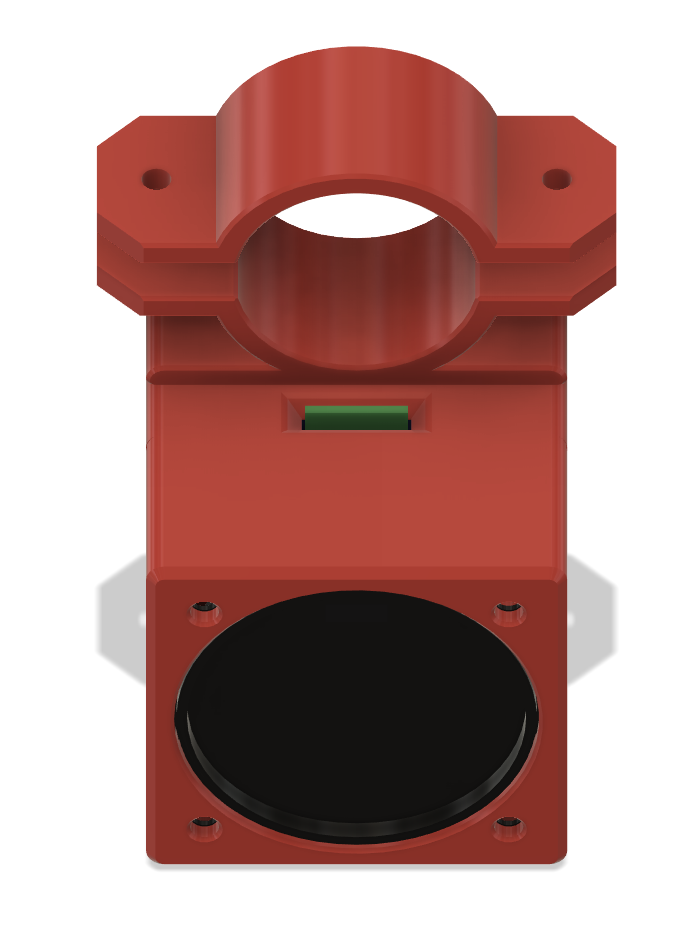
\includegraphics[width=0.25\textwidth]{graphics/final-cad.png}
		\end{wrapfigure}

		The Walking Aid Usage Prompt System is a medical aid consisting of a pair of hardware devices that allows patients suffering with dementia to be automatically reminded to use their walking aid when they begin walking without it. With stastically high rates of falling in dementia patients, the Walking Aid Usage Prompt System attempts to reduce these numbers. It aims to do this by detecting when patients are walking without their walking aid and plays them an audible reminder from a relatives voice, to take their walking aid with them.

		\paragraph{Automatic Movement Detection}\mbox{}

		With the use of an accelerometer in each device, our systems can automatically detect when your patient is moving, and if they are moving without their walking aid.

		\paragraph{Remind the patient with the sound of a familiar voice}\mbox{}

		Utilising the SD card reader on the walking aid device, you can upload an MP3 file to be played to the patient when they begin walking without their walking aid. The connected speaker will give you the peace of mind that the patient will hear the reminder whenever it needs to be played. According to our research, and insight from the client, this will increase the chances of the patient reacting appropriately, and will ease them into being accustomed to the device.

		\begin{wrapfigure}[6]{L}{0.25\textwidth}
			\vspace{-1em}
			\centering
			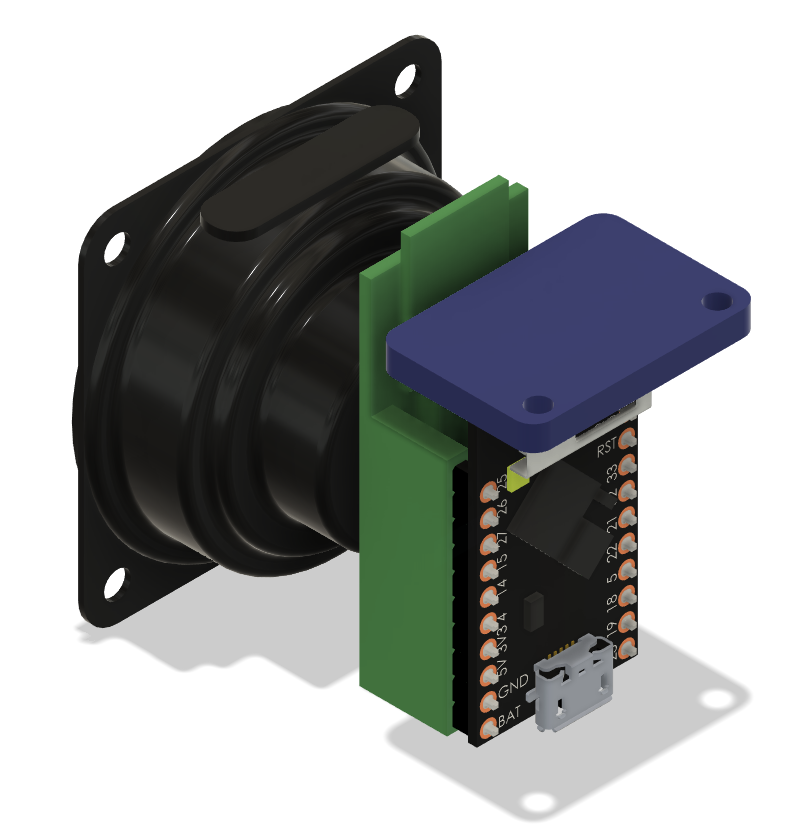
\includegraphics[width=0.25\textwidth]{graphics/hardware.png}
		\end{wrapfigure}

		\paragraph{Use vibration feedback as a reminder for patients who are hard of hearing}\mbox{}

		The inclusion of a low power, low latency communication protocol between our two devices will mean that the use of an audio reminder can be replaced, with the wearable device being asked to vibrate instead.

		\newpage

		\paragraph{Never use intrusive wearables again}\mbox{}

		Boasting a small form factor and the avoidance of distracting LEDs, our devices were developed with the comfort of the patient in mind. Utilising 18mm x 32mm TinyPICO development boards, our solution succeeds at keeping device sizes to a minimum and can be worn on either the ankle or wrist, with adaptable attachment methods that can be tailored to each patient.

		\vspace{5em}
		\paragraph{Next Steps:}\mbox{}

		\vspace{1em}
		Excited to get started?

		\textit{\hyperref[sec:quick_start_guide]{Click here for our Quick Start Guide} or head to section \ref{sec:quick_start_guide}}

		\vspace{1em}
		Want to learn more?

		\textit{\hyperref[sec:user_guide]{Click here for our more in depth User Guide} or head to section \ref{sec:user_guide}}

		\vspace{1em}
		Are you a developer?

		\textit{\hyperref[sec:developer_guide]{Click here to head to our developer guide} or head to section \ref{sec:developer_guide}}

	\newpage
	\section{Quick Start Guide}
	\label{sec:quick_start_guide}

		\subsection{Introduction}
		\label{subsec:quick_start_guide_introduction}

			The Walking Aid Usage Prompt system is a medical aid that allows patients to be automatically reminded to use their walking aid when they begin walking without it. The whole system comprises of two separate devices, one to be attached to the user's walking aid and the other to the ankle or wrist of the user. The wearable device is used to detect when the user has taken 5 steps within a 10 second period to signify that the user has began walking. Once this occurs, the wearable device communicates with the user's walking aid device to make a check to see if the walking aid is moving also. If the walking aid is moving, then great! There is no need to worry, the user is making use of their walking aid. However, should a user not be utilising their walking aid, then the walking aid can either play an audio reminder to the user, or it can communicate back to the wearable device to vibrate against the ankle or the wrist of the user. Both solutions are designed to remind the user to take their walking aid with them when walking in an attempt to reduce fall rates in dementia patients.

			The remainder of this quick start guide will explain the prerequisites to ensure that the system is fully functional, and a brief setup guide so that the user can get started.

		\subsection{Hardware Requirements}
		\label{subsec:quick_start_guide_hardware}

			\paragraph{To use the audio reminder system:}\mbox{}

			\begin{itemize}
				\item MicroSD Card >= 2MB Capacity.
				\item Windows/MacOS/Linux Computer System.
				\item A means to read/write to the SD card from the computer system. For example, a USB to MicroSD card reader.
				\item A microphone to record audio, or a pre-recorded audio file (.MP3)
			\end{itemize}

			\paragraph{To use the vibration reminder system:}\mbox{}

			No additional hardware necessary, please advance to section \ref{subsec:quick_start_setup_guide}.

		\subsection{Software Requirements}
		\label{subsec:quick_start_guide_software}

			\paragraph{To use the audio reminder system:}\mbox{}

			\begin{itemize}
				\item Voice recording software such as Windows Voice Recorder or Audacity. (An alternative could be to record your voice message on a mobile device and transfer it to the computer system).
				\item File explorer software to copy the file to the SD card.
				\item MP3 audio file should be <= 2MB in size.
			\end{itemize}

			\paragraph{To use the vibration reminder system:}\mbox{}

			No additional software necessary, please advance to section \ref{subsec:quick_start_setup_guide}.

		\subsection{Setup Guide}
		\label{subsec:quick_start_setup_guide}

			\subsubsection{To use the audio reminder system}

				\paragraph{Getting your MicroSD card ready}\mbox{}

				To utilise the audio reminder system, you will need a MicroSD card with at least 2MB of storage capacity and an MP3 file that is less than 2MB in size. You will also need to ensure that you have a means for connecting the MicroSD card to your computer system or mobile device to ensure that the audio file can be transferred to it.

				\paragraph{Recording your reminder message}\mbox{}

				Using voice recording software and a microphone, record your voice message. The audio file should be in the .MP3 format, and we recommend that the audio file has a sample rate of 44.1kHz and a 128kbps bitrate. It is imperative that the audio file is less than 2MB in size, otherwise the full file cannot be transferred to the walking aid device.

				\paragraph{Getting ready to transfer your file to the MicroSD card}\mbox{}

				It is crucial that your MicroSD card is using a FAT16/FAT32 file system to allow our devices to detect your audio file. Should it not be using a FAT16/FAT32 file system, then please format it so that it is. WARNING! Formatting your MicroSD card will cause you to lose any existing data on it.

				\paragraph{Transferring your MP3 file to the MicroSD card}\mbox{}

				Once the MicroSD card has been connected to your computer system or mobile device, please ensure that your rename your MP3 file to \textit{reminder.mp3} and copy the file to the MicroSD card. Ensure that the audio file is contained within a folder named \textit{reminder} within the MicroSD card.

				The process is now complete! You are ready to insert the MicroSD card into the walking aid device to begin using the system.

				\paragraph{Inserting you MicroSD card into the walking aid device}\mbox{}

				\begin{wrapfigure}{R}{0.25\textwidth}
					\vspace{-3.5em}
					\centering
					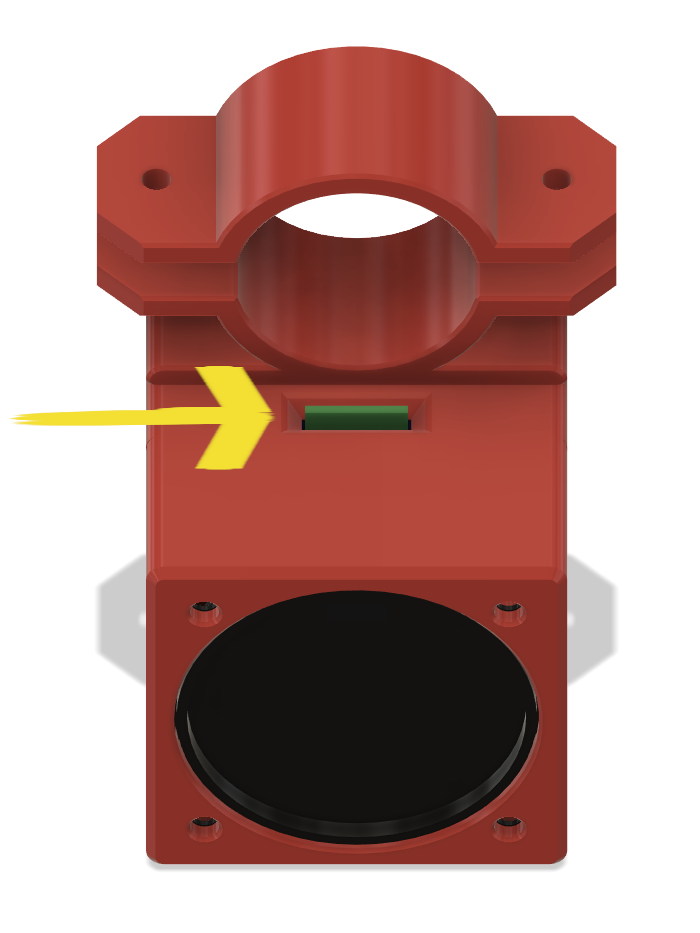
\includegraphics[width=0.25\textwidth]{graphics/sd_arrow.png}
				\end{wrapfigure}

				Once you have transferred your MP3 file to the MicroSD card, you will need to insert the MicroSD card into the walking aid device. You can insert the MicroSD card into the walking aid device by simply sliding the MicroSD card into the slot until you feel a click. The location of the MicroSD card slot can be seen in the image to the right. Once you have inserted the MicroSD card into the walking aid device, you are ready to power on your devices. Ensure that the MicroSD card is connected to the walking aid device before powering the device on.

				\paragraph{Powering on your devices}\mbox{}

				Our current prototype does not include an internal battery, but different battery solutions will be provided as options in future work. For now, the devices require 5V USB power, either from a battery bank, computer system, or phone charger. Once you have powered on your devices, you are ready to begin using the Walking Aid Usage Prompt System. To confirm that the device is functional, you should see the flash of a green LED for about one second.

				Should you notice any other LED light indicators, then please refer to the User Guide \hyperref[sec:user_guide]{here} or head to section \ref{sec:user_guide} for further troubleshooting instructions.

				\subsubsection{To use the vibration reminder system}

				As you are relying on the vibration reminder system, there is no need to utilise a MicroSD card, therefore you can skip to powering on the device. The design of our current prototype means that we will have setup the devices prior to you receiving them to ensure that they are functional for vibration reminders. Future work will be carried out to ensure that a button or switch system is implemented to allow the user to switch between vibration and audio reminders themselves.

				\paragraph{Powering on your devices}\mbox{}

				Our current prototype does not include an internal battery, but different battery solutions will be provided as options in future work. For now, the devices require 5V USB power, either from a battery bank, computer system, or phone charger. Once you have powered on your devices, you are ready to begin using the Walking Aid Usage Prompt System. To confirm that the device is functional, you should see the flash of a green LED for about one second.

				Should you notice any other LED light indicators, then please refer to the User Guide \hyperref[sec:user_guide]{here} or head to section \ref{sec:user_guide} for further troubleshooting instructions.

	\newpage
	\section{User Guide}
	\label{sec:user_guide}

		\subsection{Introduction}

			The Walking Aid Usage Prompt System is a pair of hardware devices that communicate with each other to ensure that dementia patients are utilising their walking aids when walking. The system was designed such that one device is attached to the walking aid device, which includes the MicroSD card reader and external speaker necessary for the reading and playing of the audio reminder. The other device is designed to be worn on the patient's wrist or ankle and is capable of detecting when the patient is walking as well being capable of playing a vibration reminder to the patient if desired. When the wearable device has detected that the patient has walked 5 steps within a 10 second period, the walking aid device will play an audio or vibration reminder to the patient if it is not also moving. 

			This user guide details the necessary steps to setup the devices ready for use along with instructions for troubleshooting if any issues are encountered.

		\subsection{Hardware Requirements}
		\label{subsec:hardware_reqs}

			\paragraph{To use the audio reminder system:}\mbox{}

			\begin{itemize}
				\item MicroSD Card >= 2MB Capacity.
				\item Windows/MacOS/Linux Computer System.
				\item A means to read/write to the SD card from the computer system. For example, a USB to MicroSD card reader.
				\item A microphone to record audio, or a pre-recorded audio file (.MP3)
			\end{itemize}

			\paragraph{To use the vibration reminder system:}\mbox{}

			No additional hardware necessary, please advance to section \ref{subsec:setup_guide}.

		\subsection{Software Requirements}
		\label{subsec:software_reqs}

			\paragraph{To use the audio reminder system:}\mbox{}

			\begin{itemize}
				\item Voice recording software such as Windows Voice Recorder or Audacity. (An alternative could be to record your voice message on a mobile device and transfer it to the computer system).
				\item File explorer software to copy the file to the SD card.
				\item MP3 audio file should be <= 2MB in size.
			\end{itemize}

			\paragraph{To use the vibration reminder system:}\mbox{}

			No additional software necessary, please advance to section \ref{subsec:setup_guide}.

		\subsection{Setup Guide}
		\label{subsec:setup_guide}

			The following section is a full setup guide that can be followed to ensure that the Walking Aid Usage Prompt System is functioning correctly. The setup guide includes similar information and instructions to the quick start guide, however it shall contain more detail. The setup of the devices for use of the vibration reminder system only requires the powering on of the devices, which will be detailed in the latter stages of this user guide. The setup of the devices utilising the audio reminder system requires the completion of the following steps:

			\begin{itemize}
				\item Preparing the MicroSD card for use.
				\item Formatting your MicroSD card
				\item Recording a voice message if one is not prepared already.
				\item Transferring the audio file to the MicroSD card.
				\item Inserting the MicroSD card into the walking aid device.
				\item Powering on the devices.
			\end{itemize}

			If you are intending on utilising the vibration reminder system, then you can click \hyperref[para:powering]{here} or head to the 'Powering on your devices' section. Otherwise, please follow the steps outlined below to ensure that the Walking Aid Usage Prompt System is functioning correctly for audio reminding.

			\subsubsection{Preparing the MicroSD card for use}

				Please ensure before proceeding that the MicroSD card has a capacity of at least 2MB. You can confirm this with the packaging of the MicroSD card or by connecting it to your computer system and checking in the Windows/MacOS/Linux file explorer.

				Before getting started with the transferring of your MP3 file to the SD card, you will need to ensure that you have a means to read/write to the SD card. For example, a USB to MicroSD card reader that can connect to your computer system or mobile device, or computer system with a built in MicroSD card reader.

				\paragraph{Formatting your MicroSD card}\mbox{}

				It is imperative that your MicroSD card is utilising a FAT16/FAT32 file system to ensure that the walking aid device functions correctly. Should your MicroSD card be using a different file system, please format your MicroSD card so that it is using a FAT16/FAT32 file system. WARNING! Formatting your MicroSD card will cause you to lose all of your data currently saved on it. Instructions for formatting your MicroSD card can be found below:

				\begin{itemize}
					\item \href{https://www.bu.edu/comtech/students/technical-guides/hardware/how-to-format-hard-drives/}{Format Instructions}
				\end{itemize}

				Once the MicroSD card has been setup with the FAT16/FAT32 file system, you can proceed to the next step, transferring the audio recording to the MicroSD card.

				\paragraph{Recording a voice message if one is not prepared already}\mbox{}

				Should you already have an audio recording prepared, then please ensure that the audio file is in an MP3 format. We also recommend that the audio file has a 44.1kHz sample rate and a 128kbps bit rate.

				Using voice recording software and a microphone, record your voice message. Recommended voice recording software includes, but is not limited to, the following:

				\begin{itemize}
					\item Windows Voice Recorder
					\item Audacity
					\item Mobile Device Voice Recording App such as Voice Recorder \& Audio Editor by TapMedia Ltd (iOS)
				\end{itemize}

				We recommend that the audio file has a 44.1kHz sample rate and a 128kbps bit rate. This can be set when configuring the voice recording software, or by using software to edit the audio file after it has been recorded.

				We also recommend recording a reminder message to the patient with a friendly voice. Friendly voices are known to provide a higher success rate than generic voices that could further confuse or frighten the patient.

				\paragraph{Transferring your MP3 file to the MicroSD card}\mbox{}

				To transfer from your computer system to the MicroSD card, you will need to ensure that your file explorer software such as Windows Explorer or MacOS Finder ready to use.

				If you have recorded your voice message using a mobile device, you can either transfer your MP3 file to the computer system using a message system such as email or by connecting your mobile device to your computer system via USB. Another option is to connect your MicroSD card to your mobile device using one of the previously mentioned adapters to allow for file transfer.

				Once you have access to writing to your MicroSD card, you are ready to transfer your MP3 file. Please follow the following steps to ensure that your MP3 file is transferred to the MicroSD card correctly to be fully functional with the Walking Aid Usage Prompt System:

				\begin{itemize}
					\item Open the file explorer software and locate your voice recorded MP3 file.
					\item Rename the file to 'reminder.mp3'.
					\item Through the file explorer software, locate your MicroSD card's storage location.
					\item Create a folder on the MicroSD card named 'reminder'.
					\item Copy and paste the 'reminder.mp3' file from your computer system/mobile device to the 'reminder' folder on the MicroSD card.
				\end{itemize}

				\paragraph{Inserting you MicroSD card into the walking aid device}\mbox{}

				\begin{wrapfigure}{R}{0.25\textwidth}
					\vspace{-3.5em}
					\centering
					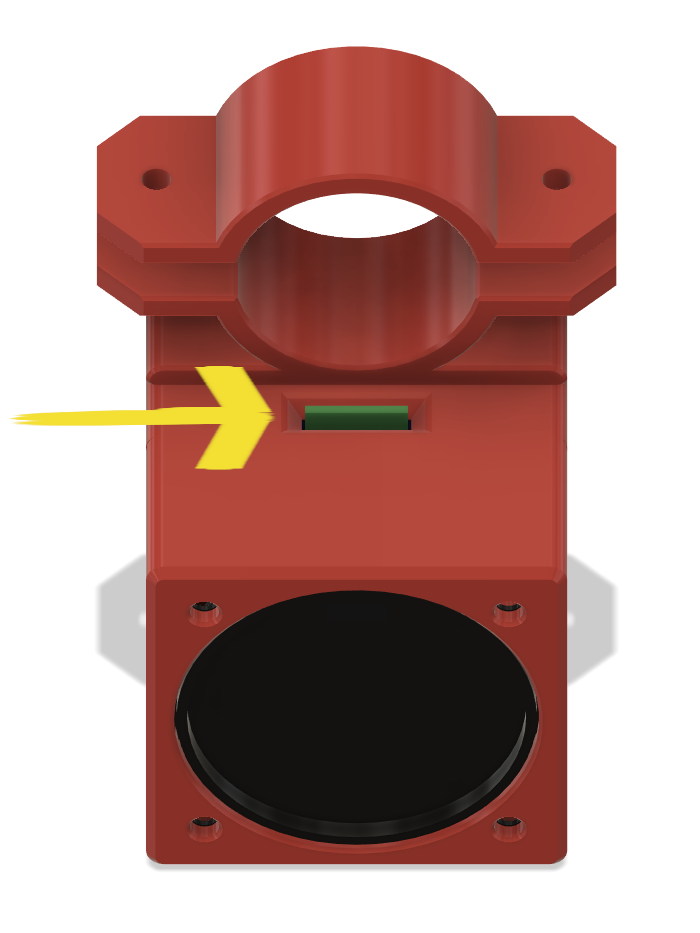
\includegraphics[width=0.25\textwidth]{graphics/sd_arrow.png}
				\end{wrapfigure}

				Once you have transferred your MP3 file to the MicroSD card, you will need to insert the MicroSD card into the walking aid device. You can insert the MicroSD card into the walking aid device by simply sliding the MicroSD card into the slot until you feel a click. The location of the MicroSD card slot can be seen in the image to the right. Once you have inserted the MicroSD card into the walking aid device, you are ready to power on your devices. Please remember that the walking aid device must have a MicroSD card inserted before the device is powered on to ensure that an audio file can be transferred to the device's onboard memory.

				\paragraph{Powering on your devices}\mbox{}
				\label{para:powering}

				If you are intending on using the vibration reminder system then the design of our current prototype means that we will have setup the devices prior to you receiving them to ensure that they are functional for vibration reminders. Future work will be carried out to ensure that a button or switch system is implemented to allow the user to switch between vibration and audio reminders themselves.

				Our current prototype does not include an internal battery, but different battery solutions will be provided as options in future work. For now, the devices require 5V USB power, either from a battery bank, computer system, or phone charger. Once you have powered on your devices, you are ready to begin using the Walking Aid Usage Prompt System. To confirm that the device is functional, you should see the flash of a green LED for about one second.

				Should you notice any other LED light indicators, then please refer to the troubleshooting LEDs guide \hyperref[subsec:troubleshooting_leds]{here} or head to section \ref{subsec:troubleshooting_leds} for further troubleshooting instructions.

		\subsection{Troubleshooting LEDs}
		\label{subsec:troubleshooting_leds}

			\begin{tabular}{ m{0.1\linewidth} m{0.8\linewidth} } 

				\vspace{2em}
				
\includegraphics[width=0.5\linewidth]{graphics/green_circle.png}
				
				& You should see this LED for one second when you initally power on the device. This indicates that your device is functional. \\ 

				\vspace{2em}
				
\includegraphics[width=0.5\linewidth]{graphics/orange_circle.png}
				
				&  You are seeing this LED because the device in question is struggling to connect to the other device. Try powering them down, moving them closer together and restarting them. If you are still experiencing issues, please contact our support team here. \\ 

				\vspace{2em}
				
\includegraphics[width=0.5\linewidth]{graphics/red_circle.png}
				
				& This LED is being displayed as the initialisation of the communication protocol has failed. Please contact our support team here. \\
				 
			\end{tabular}

	\newpage
	\section{Developer Guide}
	\label{sec:developer_guide}

		This section is designed to help developers in the future to build on top of this project, to experiment with further techniques for the main features and to allow them the opportunity to learn from our code and systems to help impact the lives of dementia patients. We understand that this project may be handed onto developers in a professional setting in future, and wanted to offer a section including the necessary details on this project to allow developers to easily understand the code and systems.

		This section will contain details on how we wired both the walking aid and wearable devices, and why we decided to wire the devices the way we did. It will also contain details on the code that we have written and will provide suggestions as to how the code can be improved moving forward. We have developed our code such that classes can be transferred seamlessly for classes that utilise more expensive hardware or more complex libraries to help facilitate the advancement of these systems in future. 

		\subsection{Wiring}
		\label{subsec:wiring}

			We had intended to include a wiring diagram here of the connections between our TinyPICO boards, the accelerometers and the audio shield. However, there seems to be a lack of software that allows for the creation of wiring models for TinyPICO boards. We have therefore decided to include a list of the connections that we have made between the devices. Following this list will be illustrations of the hardware used and their pinouts. Thus, the developer can understand how the hardware is connected and be able to reference the images to understand where the pins are located on them. The following is a list of the necessary wiring between the hardware, with the TinyPICO to ADXL345 Accelerometer section necessary for both the walking aid and wearable devices, and the TinyPICO to I2S Audio Shield necessary only for the walking aid device.

			\subsubsection{TinyPICO to ADXL345 Accelerometer}

				As it was necessary for us to utilise the SPI communication standard for the communication between the TinyPICO board and the I2S Audio Shield in the walking aid device, we were influenced to utilise the I\textsuperscript{2}C communcation standard between the TinyPICO boards and the ADXL345 accelerometer. The full wiring list for the TinyPICO to ADXL345 Accelerometer is shown below.

				\begin{itemize}
					\item TinyPICO 5V Pin (5V) \hspace{2.5em} ---> \hspace{2em} ADXL345 VCC Pin.
					\item TinyPICO Ground Pin (G) \hspace{1.15em} ---> \hspace{2em} ADXL345 GND Pin.
					\item TinyPICO SDA Pin (21)	\hspace{2em} ---> \hspace{2em} ADXL345 SDA Pin.
					\item TinyPICO SCL Pin (22)	\hspace{2.1em} ---> \hspace{2em} ADXL345 SCL Pin.
				\end{itemize}

				We opted not to utilise the INT1 and INT2 interrupt pins for this project, but they do provide an interesting experimental feature for further development work. These pins could be used to trigger a software interrupt on the TinyPICO board, which would allow code to be run in real time when an event has been triggered through the accelerometer.

			\subsubsection{TinyPICO to I2S Audio Shield}

				The TinyPICO to Audio Shield communication utilises the I\textsuperscript{2}S audio communication standard and that was why we opted for this specific wiring communication. It was also a necessity for us to use the SPI communication protocol between the two hardware devices to provide a communication route for the transferring of audio files between the two boards. The full wiring list for the TinyPICO to I2S Audio Shield is shown below.

				\begin{itemize}
					\item TinyPICO 3.3V Pin (3V3) \hspace{2.1em} ---> \hspace{2em} I2S Audio Shield 3.3V Pin (3V3).
					\item TinyPICO Ground Pin (G) \hspace{2em} ---> \hspace{2em} I2S Audio Shield Ground Pin (G).
					\item TinyPICO SS Pin (5) \hspace{4.15em} ---> \hspace{2em} I2S Audio Shield SD SEL Pin (5).
					\item TinyPICO SCK Pin (18) \hspace{2.8em} ---> \hspace{2em} I2S Audio Shield SPI CLK Pin (18).
					\item TinyPICO MI Pin (19) \hspace{3.55em} ---> \hspace{2em} I2S Audio Shield SPI MI Pin (19).
					\item TinyPICO MO Pin (23) \hspace{3.15em} ---> \hspace{2em} I2S Audio Shield SPI MO Pin (23).
					\item TinyPICO DAC 1 Pin (25) \hspace{2em} ---> \hspace{2em} I2S Audio Shield D IN Pin (25).
					\item TinyPICO DAC 2 Pin (26) \hspace{2em} ---> \hspace{2em} I2S Audio Shield LRCLK Pin (26).
					\item TinyPICO TCH 7 Pin (27) \hspace{2em} ---> \hspace{2em} I2S Audio Shield BCLK Pin (27).
				\end{itemize}

		\newpage
		\subsection{Hardware Pinouts}
		\label{subsec:hardware_pinouts}

			The following sections will contain the pinout images for the TinyPICO board, the ADXL345 accelerometer and the I2S Audio Shield. These images are provided for reference with the wiring section in section \ref{subsec:wiring}, to aid in the process of understanding the wiring of our systems and to allow developers to reconfigure the wiring of the devices themselves.

			\subsubsection{TinyPICO Board}

				The following is an image of the pinouts of the TinyPICO board \cite{tinypico}.

				% [H] means put the figure HERE, directly when you input this code.
\begin{figure}[H]
	\centering
	\captionsetup{width=1.0\linewidth}

% We set the width of the figure based on the width of one line of text on the page.
% The value can be tuned to any value in [0.0, 1.0] to scale the image while maintaining its aspect ratio.

	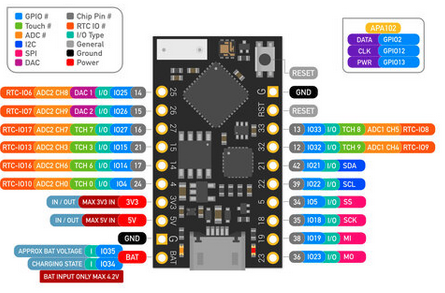
\includegraphics[width=1.0\linewidth]{graphics/tinypico_pinouts.png}

% Caption is defined with a short and long version. The short version is shown in the
% List of Figures section, and the long version is used directly with the figure.
	\caption[TinyPICO Pinouts]{An illustration of the TinyPICO pinouts provided by \cite{tinypico}}

% For figures label should be defined after the caption to ensure proper figure numbering.
	\label{fig:tinypico_pinouts}

\end{figure}

			\newpage
			\subsubsection{ADXL345 Accelerometer}

				The following is an image of the pinouts of the ADXL345 accelerometer \cite{components101}.

				% [H] means put the figure HERE, directly when you input this code.
\begin{figure}[H]
	\centering
	\captionsetup{width=1.0\linewidth}

% We set the width of the figure based on the width of one line of text on the page.
% The value can be tuned to any value in [0.0, 1.0] to scale the image while maintaining its aspect ratio.

	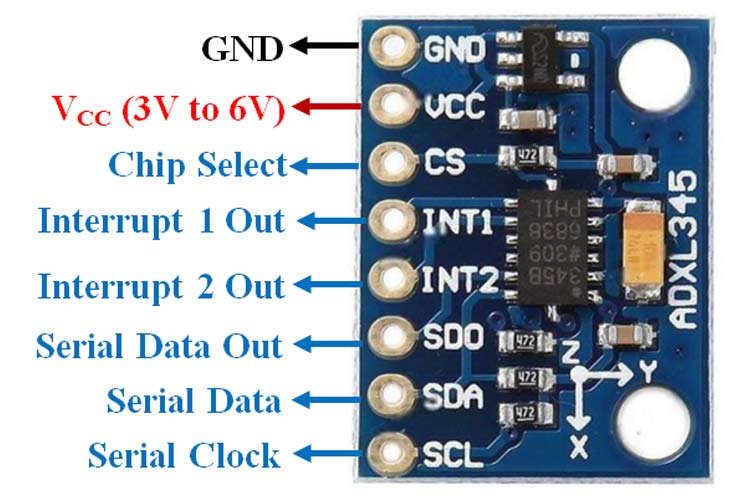
\includegraphics[width=0.75\linewidth]{graphics/accel_pinouts.jpg}

% Caption is defined with a short and long version. The short version is shown in the
% List of Figures section, and the long version is used directly with the figure.
	\caption[ADXL345 Accelerometer Pinouts]{An illustration of the ADXL345 accelerometer pinouts provided by \cite{components101}}

% For figures label should be defined after the caption to ensure proper figure numbering.
	\label{fig:accel_pinouts}

\end{figure}

			\newpage
			\subsubsection{I2S Audio Shield}

				The following is an image of the pinouts of the I2S audio shield \cite{unexpected_maker}.

				% [H] means put the figure HERE, directly when you input this code.
\begin{figure}[H]
	\centering
	\captionsetup{width=1.0\linewidth}

% We set the width of the figure based on the width of one line of text on the page.
% The value can be tuned to any value in [0.0, 1.0] to scale the image while maintaining its aspect ratio.

	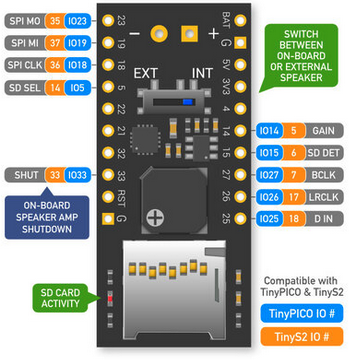
\includegraphics[width=0.75\linewidth]{graphics/audioshield_pinouts.png}

% Caption is defined with a short and long version. The short version is shown in the
% List of Figures section, and the long version is used directly with the figure.
	\caption[I2S Audio Shield Pinouts]{An illustration of the I2S audio shield pinouts provided by \cite{unexpected_maker}}

% For figures label should be defined after the caption to ensure proper figure numbering.
	\label{fig:audioshield_pinouts}

\end{figure}

		\newpage
		\subsection{Software Development}

			This section is designed to help the developer understand what each class within the software system does and how they can be altered to incorporate different technologies that could potentially improve the system in future. Each breakdown of the classes will include an overview of what the class does, and what particular changes can be made to adjust the system.

			\subsubsection{WalkAidAccelerometer/WearableAccelerometer}

				These classes are used to operate the walking and movement detection features of the wearable and walking aid devices. They currently utilise a system that detects changes in gravity over a specified threshold as steps. Those steps are recorded as the steps those devices have taken and signify whether they are moving or not. Issues relating to this system can also be identified in high end mobile step counters, where the quick movement of the mobile device without actually walking can cause steps to be detected.

				Listing \ref{lst:accel} demonstrates how the code is implemented to detect changes in gravity and call the code that increments the step counter on the wearable device and the last step time updater on the walking aid device. This code can be easily replaced with code that detects changes in acceleration for example. An interesting alternative here could be to implement distance tracking between the two devices with the accurate Ultra wideband technology currently on offer. However, this technology would add to your budget. 

				\lstinputlisting[language=C++, caption=Code to detect steps through the ADXL345's built-in single tap detection feature., label=lst:accel]{listings/tap_detection.cpp}

				Both accelerometer classes also contain initialisations of the accelerometer, which is used to set the threshold for the single tap detection feature. We encourage the developers to experiment with different thresholds to see how the system performs for your specific needs. A further feature that could be experimented with is the use of the interrupt signals sent by the accelerometer. Utilising the INT1 or INT2 pins on the ADXL345 could allow the user to call a function in real time when an event has been triggered through the accelerometer.

				Further documentation for these classes can be viewed in sections \ref{subsec:WalkAidAccelerometer} and \ref{subsec:WearableAccelerometer}.

			\subsection{WalkAidCommunications/WearableCommunications}

				These classes are used to define the communication behaviours between the walking aid and wearable devices. As mentioned previously, we opted to utilise ESP-Now as our communication protocol, but this technology can be easily transferred to the developer's preferred technology such as Bluetooth. The classes in their current form include an init class that initialises the necessary details for ESP-Now to function correctly within this system. This includes the assigning of peer devices and messages that should be sent to those peer devices. 

				Within the main sketch files of each device, we include the callback function OnDataRecv, which is called when ESP-Now detects a message. It is here that the developer can adjust the behaviour of the system when the message received. For example, we currently use the code in listing \ref{lst:callback} on the walking aid device to set a boolean to true, which in turn allows the next run of the Arduino loop function to check if the walking aid is moving. This can be adjusted however to incorporate the needs of the developer. For example, the developer could instead opt to use a different method for movement detection and have that function called within the callback function.

				\lstinputlisting[language=C++, caption=A callback function called when the walking aid device detects a message., label=lst:callback]{listings/callback.cpp}

				Further documentation for these classes can be viewed in sections \ref{subsec:WalkAidCommunications} and \ref{subsec:WearableCommunications}.

			\subsection{WalkAidAudio}

				The WalkAidAudio class handles the initialisation of the SDToSPIFFS class, calls for the audio file to be transferred from the SD card to the SPIFFS file system, and then calls for the audio file to be played when necessary. The class currently utilises a select number of generator classes to allow the ESP32 to interpret the MP3 file. The developer can adjust these classes to allow for further audio file formats to be interpreted also.

				The playing of the audio file requires the reinstantiation of these audio generators and decoders before allowing the audio to be played correctly.

				Further documentation for this class can be viewed in section \ref{subsec:WalkAidAudio}.

			\subsection{SDToSPIFFS}

				To allow for the transferral of the MP3 file from the MicroSD card to the SPIFFS file system, the SDToSPIFFS class is used. The class utilises the SdFat library discussed in section \ref{subsec:sdfat}. We opted to utilise this class due to the inefficiency of Arduino's SD library, we highly recommend that the developer avoids the use of the Arduino SD library due to these inefficiency reasons. Our current system requires that the MicroSD card is within the MicroSD card slot of the walking aid device whenever it is powered on. This is due to the fact that the SPIFFS file system is volatile and therefore data within it is deleted when the device powers down. A future advancement to this could involve the developer adjusting our code in listing \ref{lst:transfer} to allow for the transferral of the MP3 file to a persistent storage location, or to include code that detects when a MicroSD card has been inserted and have the transferral process take place at that point. 

				\lstinputlisting[language=C++, caption=Code to transfer the MP3 file from the MicroSD card to the SPIFFS file system., label=lst:transfer]{listings/transfer.cpp}

				Further documentation for this class can be viewed in section \ref{subsec:sdtospiffs}.

			\subsection{Sketch Files}

				The sketch file for each device contains the functions necessary to allow the devices to be developed through Arduino. The setup function of each class instantiates the required libraries for the full desired functionality of the systems. The loop function for the wearable device repeatedly calls the check for step function where steps are detected and added to the counter, and calls for messages to be sent to the walking aid device are made should a reminder need to be played.

				The loop function for the walking aid device is a little more complex as it incorporates the functionality for checking if the walking aid had been moved in the last 10 seconds and if not, waits to see if the walking aid is moved in the next 10 seconds before deciding to play a reminder or not. The code for the walking aid loop function can be viewed in listing \ref{lst:loop}. The main area we feel that the developer could experiment with here is to implement the accelerometer interrupt feature to allow movements to be responded to in real time rather than having to wait for the loop function to be called each time to have movements detected.

				\lstinputlisting[language=C++, caption=The loop function of the walking aid sketch file., label=lst:loop]{listings/loop.cpp}

				Further documentation for these sketch files can be viewed in sections \ref{subsec:sketch_walking_aid} and \ref{subsec:sketch_wearable}.

	\chapter{Narrative and Reflective Account}
\label{ch:narrative}

    In this chapter, we will provide a detailed narrative and reflective account as well as a perspective on the entire process of developing the Walking Aid Usage Prompt System. Specifically, in this chapter, we will describe the development process, from the beginning to the end, along with all the problems we encountered, and how we solved them.

    \section{Requirements and Topic}
    \label{sec:reqs}

    The first thing we did was to arrange a meeting with the client, who in this case was a representative of Bangor Health Clinic. The reason for this meeting is to understand better the topic and also gather the requirements from the client. At first, we thought of two possible outcomes, according to the client's requirements, developing a wearable device or a non-wearable device. The first one is a device similar to a watch that will include an accelerometer, which will be responsible for calculating the user's movement, and the second one is a pressure pad, that will detect when the user is sitting or not to it. We proposed to Bangor Health Clinic, the first solution rather than the second, as the second might need extra information to calculate the user's movement, for instance, if the user stands up there is no way of understanding if the user is walking, or creating a solution in which the pad can be easily cleaned up. All of these reasons were also very difficult for us to implement, so we chose the first solution as it is the more passable solution when it comes to our skills.

    \section{Development}
    \label{sec:development}

    The next step is the development of the proposed solution, including the methodology we followed. The development of the Walking Aid System was tough for our team, to complete in time, as we lost valuable time at the beginning of the project while waiting for the proper equipment to arrive. Fortunately, we moved the project forward in both software and hardware development, developing prototypes, after their arrival. The loss of that time was something from which our timetable could never recover. Although we realized that working on a project that includes both software and hardware development may necessitate additional time, the delivery and arrival of the equipment may take extra time; therefore, the project plan must be adaptable to those dates. The development is split into three sections, the first section contains all the problems we encountered for the software development, the second section contains all the problems we encountered for the hardware development, and the final one contains all the problems we encountered for the risk analysis. Each section will highlight how we solved the problem if it was solved, and what we learnt from that solution.

    \subsection{Software Development}
    \label{ssec:software}

    Working on this type of project that requires software and hardware development was very challenging for us, especially when it comes to hardware selection, which was the first problem we faced. Because the initial budget we required exceeded the one allocated by the customer, we devised a method to reduce the ordering budget by borrowing two TinyPICOs from the University. Having now all the equimpent we needed to find a solution on how these two systems will communicate with each other. Choosing a communication protocol was a key challenge since we required one that would not exceed our budget while still being extremely precise at a long-range. As a result, we chose the ESP-Now protocol for communication between our TinyPICOs since it is simple to integrate with ESP32 chips and has a range of 220 meters.

    % Add more information about walking detection system, problems and solutions.

    \subsection{Hardware Development}
    \label{ssec:hardware}

    % What problems we encountered during this phase, and what are our solutions.
    % What we learnt from the problem(s) and the solution(s)

    \subsection{Risk Analysis}
    \label{ssec:}

    % What problems we encountered while defining risks
    When we defined our risks in Milestone 1 \cite{coaker}, we ran into issues with our budget and hardware procurement, which caused us to lose development time as mentioned in the previous section \ref{sec:development}. However, in Milestone 2 \cite{mile2}, we revised our risks because the loss of development time was still affecting our schedule, so we needed to conduct team meetings so we could oversee the project's progress, whether we were still behind schedule or not.

    \section{Reflection}
    \label{sec:Reflection}

    From this group project, the first thing we learnt from developing a project for a client is that working in groups is very difficult, especially when not all members contribute at the same level. This is something that happened in this project, as some members did not pull their weight, resulting in many incomplete tasks being left to be completed at the last minute. This might have happened since everyone's schedules were different, but it doesn't imply it's not a reasonable reason for everyone's workload. Of course, if all of the team members were equally devoted to this project, we would have greater outcomes and not have as much work to do near the finish.

    Needless to say, given this was a group project, we had to hold meetings to maintain track of the project's development. Using Discord for our meetings eased and simplified things for us. In addition, we used GitHub, which improved our git expertise and made it easy for us to divide the documentation work and all of the project's work in general.

    Although, this project gave us the chance to implement software engineering principles we learnt through the years of our studies, such as software design, choosing a proper methodology, developing a project plan and also working as a team.


% Formatting citations properly when they are rendering incorrectly in your PDF can be fiddly,
% espectially when punctuation and international characters are involed. Sometimes multiple re-compilations
% are needed in addition to clearing temporary auxiliary files to see your changes in your document.
% Insert the bibliography using citations contained in the file citations.bib
	\bibintoc
	\bibliography{citations}

\end{document}
